\documentclass{article}
\usepackage[backend=biber, citestyle=authoryear, bibencoding=utf8]{biblatex}
\addbibresource{./bibs/vlab-report.bib}
\addbibresource{./bibs/unicef-ie.bib}
\usepackage{adjustbox}
\usepackage{graphicx}
\usepackage[utf8]{inputenc}
\usepackage{geometry}
\usepackage{lscape}
\usepackage{csquotes}
\usepackage{float}
\usepackage{amsmath}

\usepackage{caption}
\usepackage{subcaption}

\usepackage{dcolumn}
 \geometry{
 a4paper,
 total={170mm,257mm},
 left=10mm,
 top=10mm
 }

\title{Bebbo}
\date{February 2024}

\begin{document}

\maketitle

\tableofcontents

\clearpage
\section{Executive Summary}

To support parents to receive timely and quality guidance even when direct contact with service  providers is not possible and overcome barriers in access to localized digital solutions with verified  content, UNICEF Europe and Central Asia Regional Office (ECARO) developed a mobile parenting app,  Bebbo. The mobile application also supports the most vulnerable parents/caregivers with lower  education level, in terms of the navigation modalities, off-line operability and selection of the core  content. The two main objectives of Bebbo, in line with the UNICEF ECARO Early Childhood  Development Theory of Change, are: (1) Improving availability of information for parents on child  development, and (2) Supporting parents for responsive caregiving and early intervention.  Accordingly, Bebbo app provides users information and interactive tools to help nurture and aid their  child’s health and development. The launch of Bebbo in 11 countries in the ECA region is a direct  response to the identified objective to engage parents and caregivers in nurturing care, positive  parenting, and stimulating learning.

\subsection*{The Context}
Parents everywhere are in need of information on various aspects of child development from reliable  and validated sources as well as guidance on how to support the health and development of their  children. However, services providing this sort of information and support are often non-existent or  inaccessible for a lot of parents in many places. Often, service providers, even when accessible, might  lack necessary knowledge and skills to respond to the questions and concerns parents might have.

Mobile apps are one of the most convenient and easy ways to access information about child  development and parenting. However, parenting apps are mainly in English and provide a limited  thematic content without a possibility for parents to familiarize with, track, and support all aspects of  their child’s health and development. In addition, these apps are, naturally, not adapted to contexts of  individual countries. Many apps are not free of charge, which presents a significant barrier, particularly  for the most vulnerable families. At the same time, the majority of the existing apps operate only in  online mode requiring good internet connectivity that is lacking in remote and rural areas.

\subsection*{The App}

The Bebbo app is designed so that parents can begin using the app by creating a "profile" of their baby, entering basic information such as when the baby was born. After this, the parent is shown relevant content, asked to track milestones, and offered suggestions for content reading or games to play with their child.

\subsection*{Impact Evaluation}

We perform a study across two countries, Serbia and Bulgaria, using a randomized encouragement design to compare the impact of encouraging caregivers of young children to use the Bebbo app as compared to a treatment-as-usual (TAU) condition of encouraging them to use a static informational website. By comparing Bebbo to the existing TAU, we are asking the question: “does this new treatment offer something above and beyond the already existing treatments which parents might presumably already be asked to do?”

We measure effects on eight outcomes across three domains: knowledge, attitudes, and practices. This study follows a randomized, difference-in-difference design, also known as a prepost design (\cite{Clifford2021}). Survey questions measuring the outcomes are asked at both the baseline (before treatment) and the endline (at least 4 weeks after treatment) surveys. Finally, an additional follow-up survey was sent (at least 4 weeks after the endline), to measure impacts of longer-term usage.

\subsection*{Results}

We do not find evidence that asking this population to use Bebbo has any impact beyond that of asking them to visit a parenting website. Given the study design, however, we can make some additional inferences and policy recommendations:

\begin{enumerate}
\item The majority of the caregiving population in these countries is already very “good” in regards to the majority of the outcomes of interest. This implies that one does not need a ``general population'' tool that is meant to work on all outcomes across all types of people. It might be more efficient to develop targeted interventions that target desired behaviors directly or target populations or communities directly.
\item Awareness is in and of itself an effective intervention for some outcomes of interest, including knowledge of vaccine requirements. We see this because participants improved from the first questionnaire to the second questionnaire, regardless of treatment arm and regardless of compliance.
\item Bebbo is engaging to a small subset of the population, who are neither more or less likely to be the people who need support. The app cannot, therefore, be expected to have a population-level impact unless it improves its engagement metrics. In our study, only 24\% of respondents who complied with the request to download the app ended up using it beyond the first day, and only 5\% used it more than three days. When analyzing app data from Serbia and Bulgaria outside of the study population, we find that only 15\% of downloaders use it more than one day and 6\% more than three days.
\end{enumerate}

These three facts highlight that promoting Bebbo not only has no measurable impact on our study population, but we would also not expect it to have a large impact on the measured outcomes in the general population in these countries. In particular, this study indicates that raising awareness alone might be a more effective intervention. We recommend that before the app be expected to have an impact on a population level the product team must improve the basic engagement, retention, and churn numbers.

At the same time, while only about 5\% of app downloaders become regular users, that does still mean that there are over 2000 users in Serbia and Bulgaria who downloaded the app in 2023 and who went on to use it regularly. That usage alone indicates that they see some value. Unfortunately, our analysis does not reveal any trend that suggests those who download are either those who need or do not need the app according to our measures. We recommend relying on qualitative research about those users to understand the true value of the app among those who do choose to download it and end up using it regularly. 


\section{Evaluation Questions}

\addcontentsline{toc}{subsection}{What question does this evaluation answer?}
\subsection*{What question does this evaluation answer?}
The design of the study is set up to answer the following question in the positive:

\begin{displayquote}
Is promoting Bebbo an effective policy to improve the parenting knowledge, attitudes, and practices of the general population of caregivers of young children in Bulgaria and Serbia?
\end{displayquote}

\noindent Note that the study cannot fully answer the question in the negative, it cannot prove that this intervention is ineffective, it can only fail to measure its effectiveness.

We are only testing the effectivess of ``asking'' or ``inviting'' parents to use the app. Alternatively, one might be interested in testing the effectiveness ``incentivizing'' or ``forcing'' parents to use the app, but we are not doing that in this evaluation. We consider ``an effective policy'' one which performs better than the ``treatment as usual'' case, which we will consider to be an existing, static website (see Study Design for details). Finally, we are studying the general population of caregivers of young children. No particular care was given to single out any particular subset of the population that might benefit the most (or the least) from Bebbo, nor those who would be most likely to use Bebbo. Given the relatively low engagement seen with the app among study participants, it might be interesting to focus future studies on the subset of caregivers who are most likely to use Bebbo, assuming that it may not be a tool for the general population.

Alternatively, it might be useful to increase the engagement of the app among a general population of caregivers, before testing its impact again on a general population.


\section{Study Design}

\addcontentsline{toc}{subsection}{Experiment Design}
\subsection*{Experiment Design}

This study follows a prepost design (\cite{Clifford2021}) in which we measure the outcomes of interest before treatment (in a baseline survey) and after treatment (in an endline survey). We add an additional survey after the endline, referred to as a follow up, to look for longer-term impacts and test the impact of continued app usage.


% \vspace{1cm}
\begin{figure}[H]
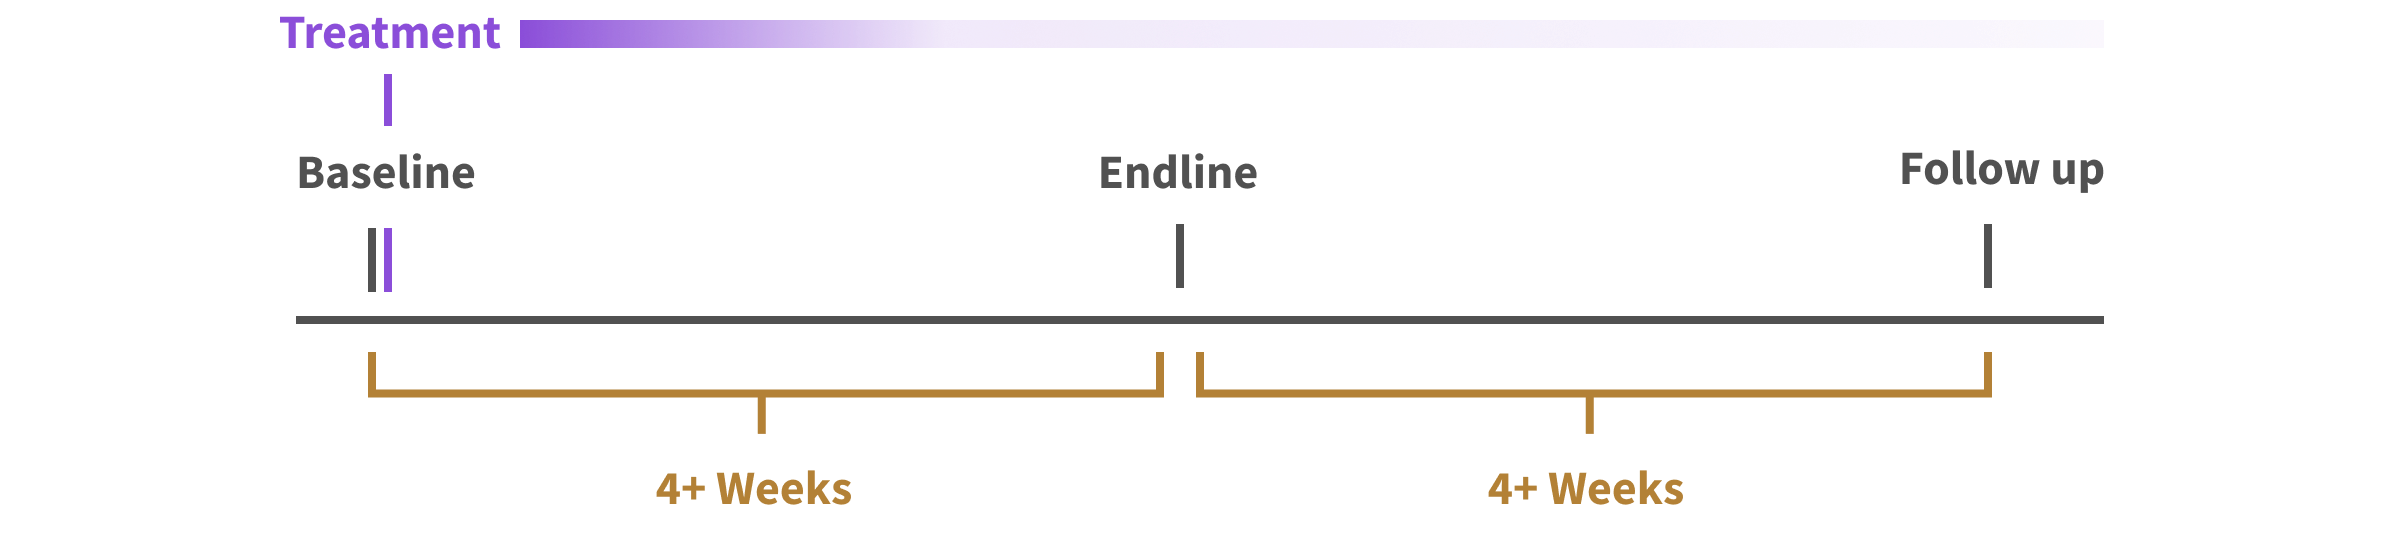
\includegraphics[width=\textwidth]{images/design-timeline.png}
\caption{Study Design}
\label{fig:Study Design}
\end{figure}

\noindent Study participants are randomized, from the beginning, to one of two conditions:

\begin{enumerate}
\item \textbf{Treatment.} Participants in the treatment condition were told that there was one more step to qualify for the study and were then asked to download the app Bebbo and use it regularly, being encouraged that doing so will help them with their parenting.
\item \textbf{Control.} Participants in the control condition were told that there was one more step to qualify for the study and were then asked to visit a parenting website and use it regularly, being encouraged that doing so will help them with their parenting.
\end{enumerate}

\noindent This follows a randomized encouragement design (\cite{Moayyedi2014}), as participants were asked to participate in the treatment, but it was not forced, thus leading to takeup that is less than 100\%. A randomized encouragement design is used here because:

\begin{enumerate}
\item We are interested in the impact of a treatment on a population where individuals can choose whether or not to take the treatment (the “compliers”).
\item The compliers and non-compliers might have different reactions to the treatment.
\end{enumerate}




\addcontentsline{toc}{subsection}{Treatment Condition}
\subsection*{Treatment Condition}

Participants were sent the following message at the end of the baseline survey:

\begin{quote}
There is just one more step to qualify for the Visa gift card of X. Please download Bebbo, the free parenting app, and discover how it can help you. Using Bebbo regularly can improve your interactions with your children and help you support their development better! You can do so by clicking the link below:
\end{quote}

Clicking on the link led them to the Bebbo app page where they were invited to download the app via the app stores (Google or Apple). App usage in the treatment group was tracked via tracking ids sent with the link to the app download page, allowing us to follow the app usage of each individual treatment participant and measure takeup. If someone decided to ignore the page, and instead went on their own to search for and download Bebbo, we would not have data on their usage. Thus, usage data and takeup should be considered a lower bound.

The Bebbo app is designed so that parents can begin using the app by creating a "profile" of their baby, entering basic information such as when the baby was born. After this, the parent is shown relevant content, asked to track milestones, and offered suggestions for content reading or games to play with their child.

We collected all app usage events. For the sake of our study, we were interested in a subset of events that represented the accessing of content or features that contained information or might impact their behavior. A set of (6) events were determined to fit the bill, namely: advise\_details\_opened, game\_details\_opened, child\_milestone\_tracked, child\_measurement\_entered, child\_vaccine\_entered, child\_health\_checkup\_entered.


\addcontentsline{toc}{subsection}{Control Condition}
\subsection*{Control Condition}

Participants were sent the following message at the end of the baseline survey:

\begin{quote}

There is just one more step to qualify for the Visa gift card of X. Please visit the following free parenting website and discover how it can help you. Using this website regularly  your interactions with your children and help you support their development better! You can do so by clicking the link below:
\end{quote}

The choice to use a website as a treatment-as-usual (TAU) condition was decided by the evaluation and program team because it represented an alternative (and traditional/existing) way to solve the problem that the Bebbo app was trying to solve. Another option that was considered was to use an alternate parenting app, but the team believed that using a website gave the best chance to detect a difference in the use of an app, rather than the specific implementation of the Bebbo app. Similarly, several websites were considered, and the most basic website (9meseca.bg) was chosen so as to be ``static'' (showing the same content to everyone rather than allowing user to create individualized profiles) so that it acted as an informational resource rather than a web app or platform which would similarly overlap with the concepts behind the Bebbo app.

The downside with choosing a treatment-as-usual condition is that if one does not find significant effects of the treatment, one cannot differentiate between the following scenarios:

\begin{enumerate}
    \item The control is effective and the treatment equally effective.
    \item Neither the control nor the treatment are effective.
\end{enumerate}

The assumption with this impact evaluation, from a policy perspective, is that the two are equally important. If the development and promotion of a new app does not improve parenting knowledge beyond what already exists in the market, then it is not an effective investment for public funds. That being said, there is some evidence in this study that allows us to differentiate between the two scenarios and determine that it is likely the latter. In particular, we conclude that neither control nor treatment condition make any significant impact on the general population above and beyond the priming effect of the baseline survey itself (to be discussed in depth in the section with results).

\addcontentsline{toc}{subsection}{Recruitment}
\subsection*{Recruitment}

Participants were recruited to the study with social media ads on the Meta platform (Facebook and Instagram) using the Virtual Lab platform to create and run the recruitment ads. The Virtual Lab platform is used to track and measure the price-per-respondent across multiple strata, solving the core problem of monitoring, computing expectations, and adjusting budget when recruiting samples via social media platforms that are representative across desired and measured characteristics.

An initial pilot study was run in Bulgaria to determine the cost effectiveness of the recruitment strategy, together with the incentive amount and mechanism. Results from the pilot indicated that it would not be possible to stratify according to the original plan and stay on budget. The decision was made to move forward with the overall plan, but drop the stratification, in order not to rethink too many parts of the study or fall behind schedule.

One important takeaway and recommendation of this study is to pilot more extensively if the initial pilot shows poor results. When an initial pilot does not provide the desired results, the timeline should be adjusted to reflect that more time is needed to redesign the study and pilot again before launching. Due to time constraints, the study was launched with learnings from the pilot and budget constraints were again run into, limiting the ability to recruit as large of a sample as originally desired in each country. Similarly, attrition between baseline and endline, which was not piloted, was worse than expected. One possible explanation is that the incentive strategy and communication was not attractive enough to respondents, leading to both high recruitment costs, long recruitment time, and higher-than-hoped-for attrition.

In exchange for participating in the study, participants were told they could receive gift cards worth up to 12 USD (in their local currency). These gift cards were delivered as \$4 visa international gift cards, which could be spent online but had to be spent for a purchase under \$4. See figure \ref{fig:Recruitment Ads} for examples of the ad material used for recruiting. Recruitment and survey administration was performed on a rolling basis between March and October, 2023. Each individual participant was treated at the end of the baseline survey and sent the endline survey 4 weeks after completing the baseline survey.

The survey was administered via a chatbot in Facebook Messenger, using the Virtual Lab platform. Respondents who clicked on the advertisements were directed to a Messenger chat with the Virtual Lab Facebook page, which did not contain any content or information related to this study. Consent was provided via chat, as well as all answers to the survey questions and the treatment condition. Gift cards were also provided via chat, using the Tremendous gift card platform to provide Visa international prepaid cards. The Virtual Lab chatbot allowed the researchers to create multi-wave surveys, with independent timing. It additionally allowed the easy provision of gift cards at the end of each wave, which is integrated into the survey directly via the platform.

[TODO: add recruitment stats]


\begin{figure}[H]
\centering
\begin{subfigure}{0.3\textwidth}
\centering

\includegraphics[width=100px]{images/recruitment/558.png}
\end{subfigure}
\begin{subfigure}{0.3\textwidth}
\centering

\includegraphics[width=100px]{images/recruitment/639.png}
\end{subfigure}
\begin{subfigure}{0.3\textwidth}
\centering

\includegraphics[width=100px]{images/recruitment/742.png}
\end{subfigure}
\caption{Recruitment Ads}
\label{fig:Recruitment Ads}
\end{figure}


\section{Descriptives}


\addcontentsline{toc}{subsection}{Respondent Characteristics by Country}
\subsection*{Respondent Characteristics by Country}

Table \ref{tbl:Baseline Respondent Characteristics} provides the baseline characteristics of the respondent population, separated by country. Note that these are also the control variables we will use in all regressions.

Generally speaking, most respondents were themselves parents (not grandparents or other caregives), women, under 35 years of age, and spoke the dominant language of the country at home. A little over half had children 0-2, compared to 2-6 years of age. Respondents in Bulgaria were more likely to have a university education (42\%) compared to those in Serbia (29\%).


% Table created by stargazer v.5.2.3 by Marek Hlavac, Social Policy Institute. E-mail: marek.hlavac at gmail.com
% Date and time: Sun, Jan 21, 2024 - 06:25:41 PM
\begin{table}[!htbp] \centering 
  \caption{Baseline Respondent Characteristics} 
  \label{tbl:Baseline Respondent Characteristics} 
\begin{tabular}{@{\extracolsep{5pt}} cccccc} 
\\[-1.8ex]\hline 
\hline \\[-1.8ex] 
Variable & Value & Bulgaria & Bulgaria \% & Serbia & Serbia \% \\ 
\hline \\[-1.8ex] 
woman & 1 & 1418 & 0.83 & 2102 & 0.80 \\ 
university & 1 &  725 & 0.42 &  748 & 0.29 \\ 
dominant\_language & 1 & 1571 & 0.92 & 2488 & 0.95 \\ 
is\_parent & 1 & 1485 & 0.87 & 2374 & 0.91 \\ 
age\_flag & 2-6 &  935 & 0.55 & 1561 & 0.60 \\ 
children\_count & 4+ &   70 & 0.04 &  279 & 0.11 \\ 
parent\_age\_flag & Over 35 &  365 & 0.21 &  550 & 0.21 \\ 
urban & 1 & 1059 & 0.62 &  941 & 0.36 \\ 
\hline \\[-1.8ex] 
\end{tabular} 
\end{table} 


\addcontentsline{toc}{subsection}{Construct Variables}
\subsection*{Construct Variables}

The outcomes of interest consist of eight constructs divided into three domains: knowledge and awareness, confidence and attitudes, and practices. The mapping between the constructs, domains, and questions that make up the constructs are laid out in table \ref{tbl:Construct Variable Mapping}.

The constructs ``Vaccine Knowledge'', ``Parenting Confidence'', and ``Breastfed'' are made up of only one question. The construct ``Activities Past 24h'' consists of a count of the number of activities, within the previous 24 hours, that the respondent has done. The construct ``Child Dev. Knowledge'' consists of a series of true/false questions, which are averaged based on whether or not the respondent answered correctly. The rest of the constructs are created by averaging of a set of likert variables.

Descriptive statistics regarding the baseline responses for the outcomes are shown in table \ref{tbl:Outcome Construct Descriptives Pooled Baseline}. Note that many of the constructs have quite high means and medians and some have a high proportion of respondents with the max score. In particular, 73\% and 72\% of respondents scored perfectly on the knowledge questions. This is problematic, as knowledge is often considered the easiest to change quickly and was a core outcome of interest for the team. Additionally, knowledge questions seem to be heavily impacted by the repeated survey effect, as discussed further down.

% Respondents skewed more towards desired responses since we observe large proportions of respondents with desired responses (coded 3 and 4) and very few with "incorrect" responses (coded 1). This pattern is stronger for some variables than others. Variables measuring Responsive Parenting PA have lesser consensus than those measuring Caregiver well-being or Parenting Knowledge. Variables $make\_fun\_of$ and $smile\_around\_child$ each have more than $60\%$ of respondents responding positively.

% We observe ceiling effect for knowledge variables $past\_24h\_play$, $name\_colors$, $know\_name\_age$, $knows\_phys\_dev$ where over 90\% of respondents have marked the correct response. We observe NAs for variables that only some respondents view based on whether the question is applicable to them. Since 28 out of 33 variable have a mean of over 0.5, the responses skew towards being correct/desired response. The Child Development Knowledge variables with more uncertainty are $alphabet$, $say\_name\_age$ and $scribble$. Variables $breastfed$ and $decrease\_stress$ measuring whether the baby was breastfed within the last 24 hours and whether the parent has techniques to decrease stress levels, also have lower means.


% Table created by stargazer v.5.2.3 by Marek Hlavac, Social Policy Institute. E-mail: marek.hlavac at gmail.com
% Date and time: Sat, Feb 10, 2024 - 03:00:33 PM
% Requires LaTeX packages: dcolumn 
\begin{table}[!htbp] \centering 
  \caption{Outcome Construct Descriptives Pooled Baseline} 
  \label{tbl:Outcome Construct Descriptives Pooled Baseline} 
\begin{tabular}{@{\extracolsep{5pt}} D{.}{.}{-2} D{.}{.}{-2} D{.}{.}{-2} D{.}{.}{-2} D{.}{.}{-2} D{.}{.}{-2} D{.}{.}{-2} D{.}{.}{-2} } 
\\[-1.8ex]\hline 
\hline \\[-1.8ex] 
\multicolumn{1}{c}{name} & \multicolumn{1}{c}{mean} & \multicolumn{1}{c}{median} & \multicolumn{1}{c}{min} & \multicolumn{1}{c}{max} & \multicolumn{1}{c}{sd} & \multicolumn{1}{c}{prop\_max} & \multicolumn{1}{c}{prop\_na} \\ 
\hline \\[-1.8ex] 
\multicolumn{1}{c}{Activities Past 24h} & \multicolumn{1}{c}{4.92} & \multicolumn{1}{c}{5.0} & \multicolumn{1}{c}{0} & \multicolumn{1}{c}{6} & \multicolumn{1}{c}{1.23} & \multicolumn{1}{c}{0.41} & \multicolumn{1}{c}{0.00} \\ 
\multicolumn{1}{c}{Parenting Confidence} & \multicolumn{1}{c}{3.34} & \multicolumn{1}{c}{3.5} & \multicolumn{1}{c}{1} & \multicolumn{1}{c}{4} & \multicolumn{1}{c}{0.65} & \multicolumn{1}{c}{0.37} & \multicolumn{1}{c}{0.00} \\ 
\multicolumn{1}{c}{Positive Practices} & \multicolumn{1}{c}{3.20} & \multicolumn{1}{c}{3.5} & \multicolumn{1}{c}{1} & \multicolumn{1}{c}{4} & \multicolumn{1}{c}{0.75} & \multicolumn{1}{c}{0.27} & \multicolumn{1}{c}{0.00} \\ 
\multicolumn{1}{c}{Attitude to Phys. Punishment} & \multicolumn{1}{c}{3.13} & \multicolumn{1}{c}{3.0} & \multicolumn{1}{c}{1} & \multicolumn{1}{c}{4} & \multicolumn{1}{c}{0.84} & \multicolumn{1}{c}{0.36} & \multicolumn{1}{c}{0.00} \\ 
\multicolumn{1}{c}{Hostile Practices} & \multicolumn{1}{c}{3.04} & \multicolumn{1}{c}{3.0} & \multicolumn{1}{c}{1} & \multicolumn{1}{c}{4} & \multicolumn{1}{c}{0.69} & \multicolumn{1}{c}{0.15} & \multicolumn{1}{c}{0.00} \\ 
\multicolumn{1}{c}{Child Dev. Knowledge} & \multicolumn{1}{c}{0.86} & \multicolumn{1}{c}{1.0} & \multicolumn{1}{c}{0} & \multicolumn{1}{c}{1} & \multicolumn{1}{c}{0.28} & \multicolumn{1}{c}{0.73} & \multicolumn{1}{c}{0.00} \\ 
\multicolumn{1}{c}{Vaccine Knowledge} & \multicolumn{1}{c}{0.72} & \multicolumn{1}{c}{1.0} & \multicolumn{1}{c}{0} & \multicolumn{1}{c}{1} & \multicolumn{1}{c}{0.45} & \multicolumn{1}{c}{0.72} & \multicolumn{1}{c}{0.58} \\ 
\multicolumn{1}{c}{Breastfed} & \multicolumn{1}{c}{0.37} & \multicolumn{1}{c}{0.0} & \multicolumn{1}{c}{0} & \multicolumn{1}{c}{1} & \multicolumn{1}{c}{0.48} & \multicolumn{1}{c}{0.37} & \multicolumn{1}{c}{0.58} \\ 
\hline \\[-1.8ex] 
\end{tabular} 
\end{table} 



\addcontentsline{toc}{subsection}{Reliability Analysis}
\subsection*{Reliability Analysis}

The outcomes consist of ``constructs,'' some of which combine the answers to multiple questions into one value. The theory is that these questions are measuring the same underlying construct and that the reliability of the construct is increased by combining multiple answers.

We test this assumption, that they are measuring the same underlying construct, by looking for internal consistency using Chronbach's alpha within the variables associated with each construct. Note that all constructs are composed of either Likert scale variables or Binary scale variables and not both. In all cases, each variable is attempting to measure a unidimensional construct on the same scale, implying that Chronbach's alpha is a reasonable measure (\cite{Tavakol2011}).

This technique was used to finalize the construct/variable mapping after the data collection completed but before the analysis began, as some of the constructs had a lower internal consistency than hoped. Table \ref{tbl:Reliability: Pooled Alpha Matrix} summarizes raw and standardized alpha of each construct as used in the final analysis, along with the number of variables in it.

Constructs with a reliability above 0.70 are considered internally consistent. After initial reliability analysis, the evaluation team iteratively dropped variables or modified constructs to ensure high reliability. In all cases, the variables that were dropped were clearly not measuring the same construct or measuring it on the same scale. The construct created from Activities in the Past 24 hours initially had the lowest reliability, possibly because some of the activities might be negatively correlated. Because of this, we decided to use the sum of the variables rather than the mean, removing any concern of internal consistency and rendering the low Chronbach's alpha irrelevant. This was not the original intention of the survey creators, however, it was decided that it was more intentional to measure the construct in this fashion and there was precendence in UNICEF work ([TODO: add reference]).


% Table created by stargazer v.5.2.3 by Marek Hlavac, Social Policy Institute. E-mail: marek.hlavac at gmail.com
% Date and time: Mon, Mar 18, 2024 - 11:41:57 PM
% Requires LaTeX packages: dcolumn 
\begin{table}[!htbp] \centering 
  \caption{Reliability: Pooled Alpha Matrix} 
  \label{tbl:Reliability: Pooled Alpha Matrix} 
\begin{tabular}{@{\extracolsep{5pt}} D{.}{.}{-2} D{.}{.}{-2} D{.}{.}{-2} D{.}{.}{-2} } 
\\[-1.8ex]\hline 
\hline \\[-1.8ex] 
\multicolumn{1}{c}{construct} & \multicolumn{1}{c}{variable count} & \multicolumn{1}{c}{raw.alpha} & \multicolumn{1}{c}{std.alpha} \\ 
\hline \\[-1.8ex] 
\multicolumn{1}{c}{Vaccine Knowledge} & \multicolumn{1}{c}{1} & \multicolumn{1}{c}{} & \multicolumn{1}{c}{} \\ 
\multicolumn{1}{c}{Child Dev. Knowledge} & \multicolumn{1}{c}{4} & \multicolumn{1}{c}{0.82} & \multicolumn{1}{c}{0.82} \\ 
\multicolumn{1}{c}{Parenting Confidence} & \multicolumn{1}{c}{2} & \multicolumn{1}{c}{0.75} & \multicolumn{1}{c}{0.76} \\ 
\multicolumn{1}{c}{Attitude to Phys. Punishment} & \multicolumn{1}{c}{1} & \multicolumn{1}{c}{} & \multicolumn{1}{c}{} \\ 
\multicolumn{1}{c}{Breastfed} & \multicolumn{1}{c}{1} & \multicolumn{1}{c}{} & \multicolumn{1}{c}{} \\ 
\multicolumn{1}{c}{Activities Past 24h} & \multicolumn{1}{c}{6} & \multicolumn{1}{c}{0.56} & \multicolumn{1}{c}{0.57} \\ 
\multicolumn{1}{c}{Positive Practices} & \multicolumn{1}{c}{4} & \multicolumn{1}{c}{0.84} & \multicolumn{1}{c}{0.84} \\ 
\multicolumn{1}{c}{Hostile Practices} & \multicolumn{1}{c}{4} & \multicolumn{1}{c}{0.74} & \multicolumn{1}{c}{0.74} \\ 
\hline \\[-1.8ex] 
\end{tabular} 
\end{table} 



% \clearpage

% \section*{Baseline Construct Distributions}

% 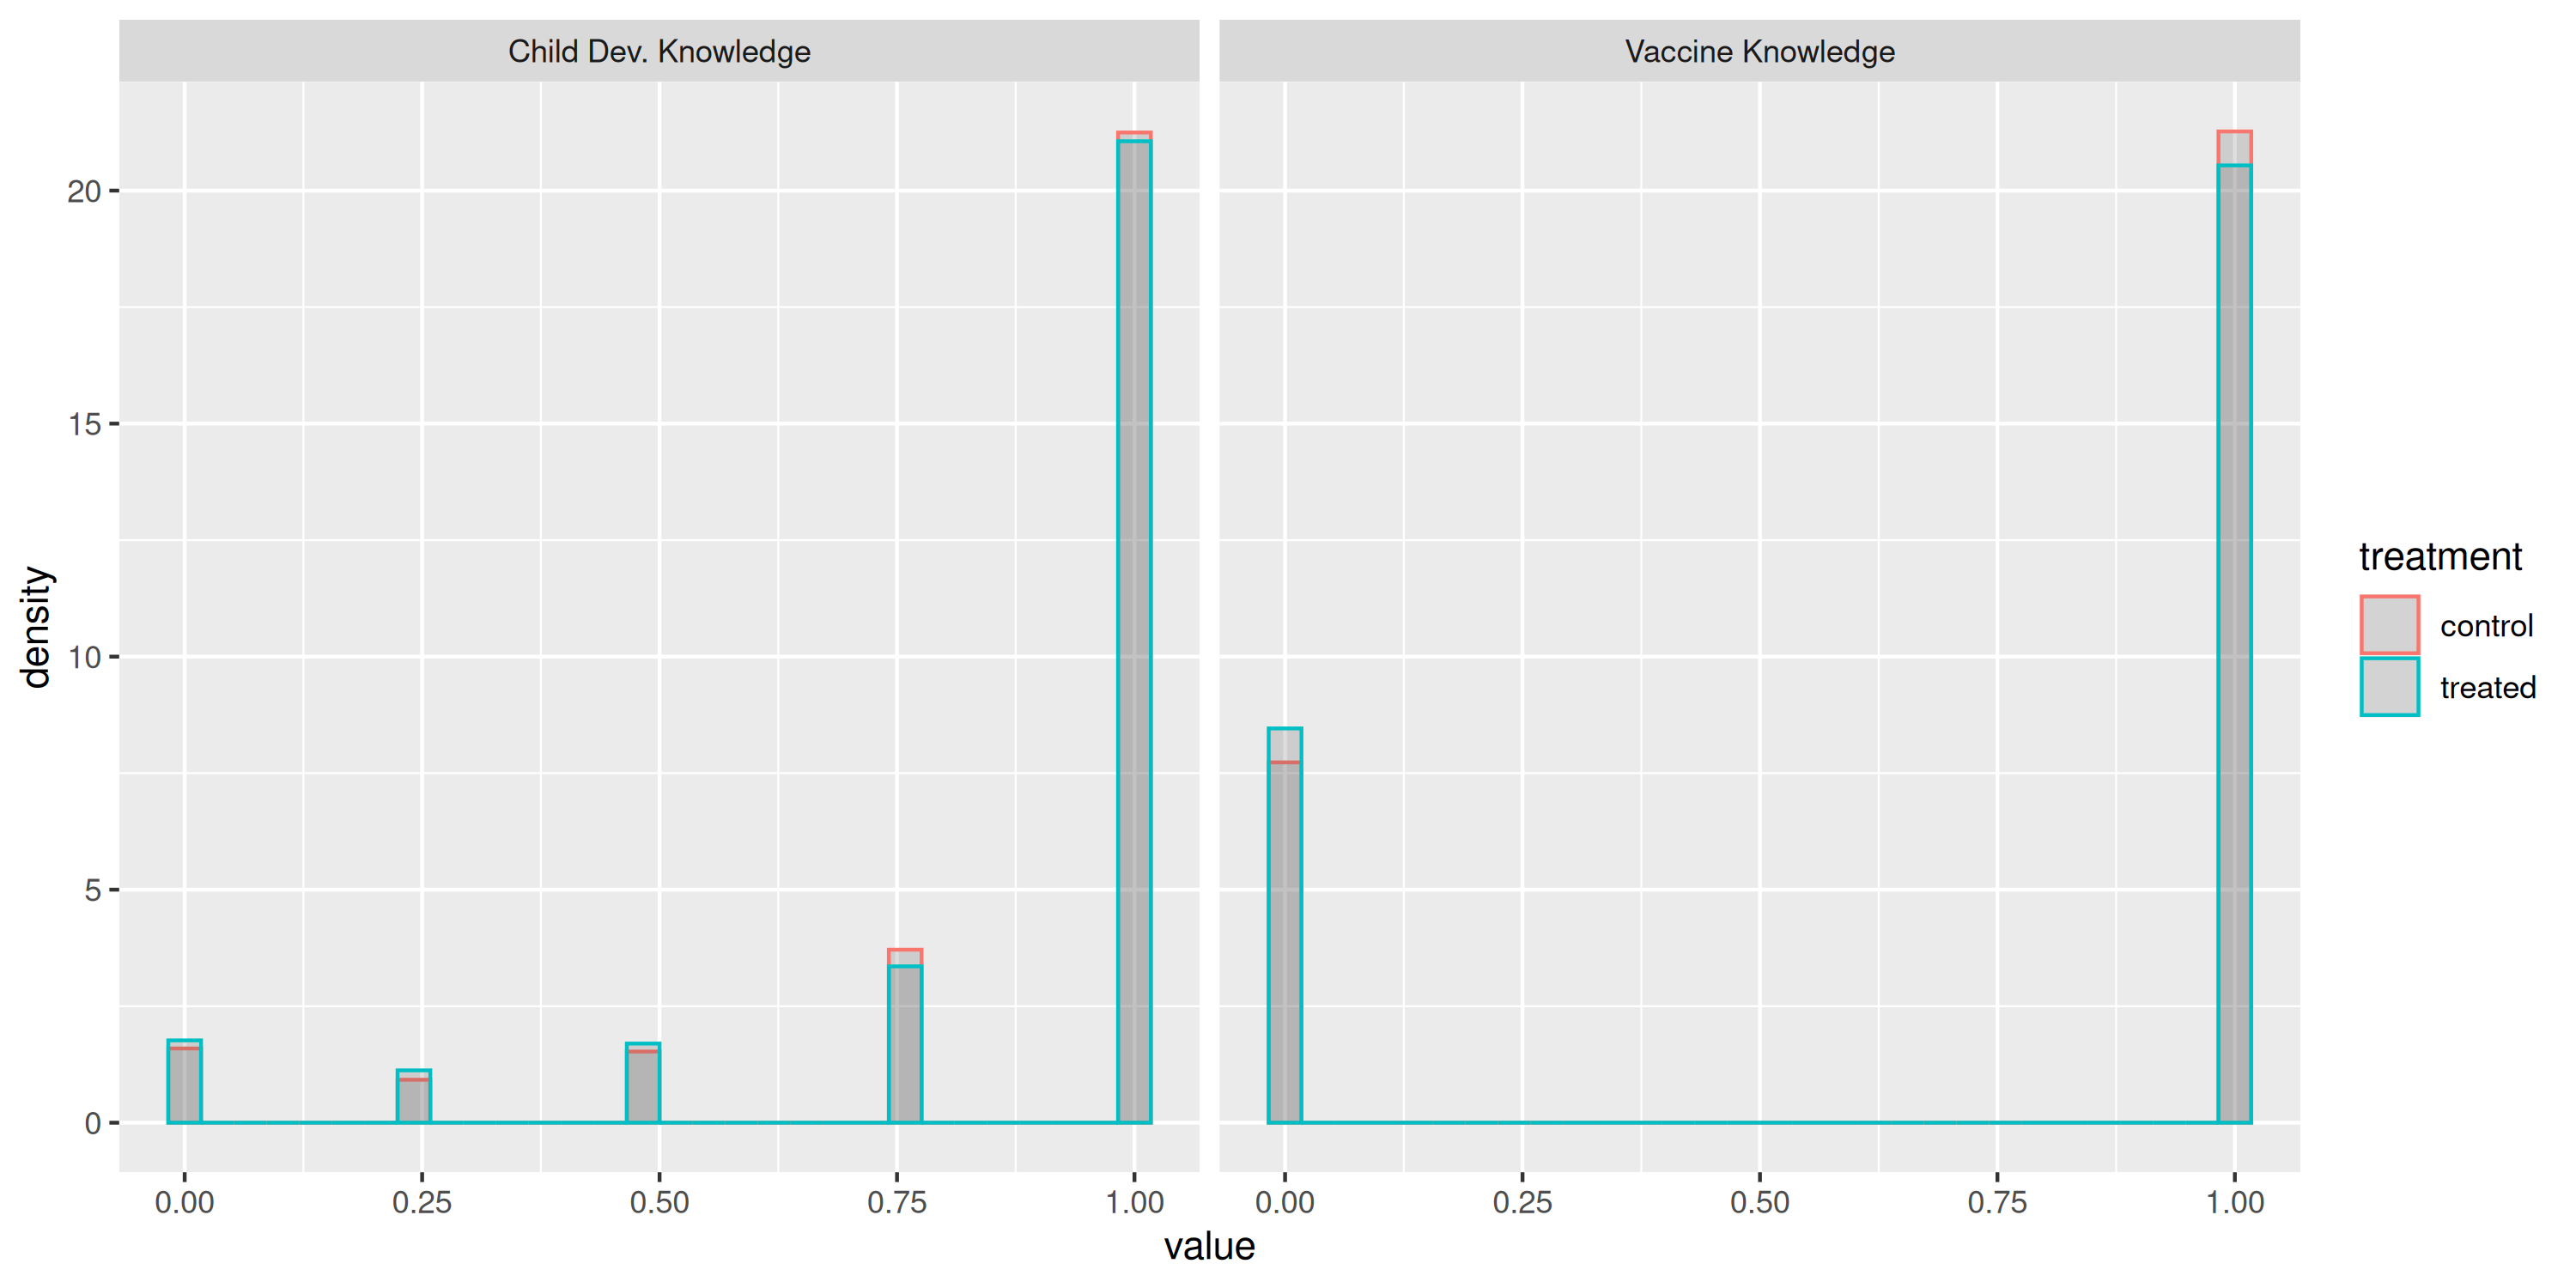
\includegraphics[width=\textwidth]{plots/Original Data - Knowledge and Awareness.png}
% 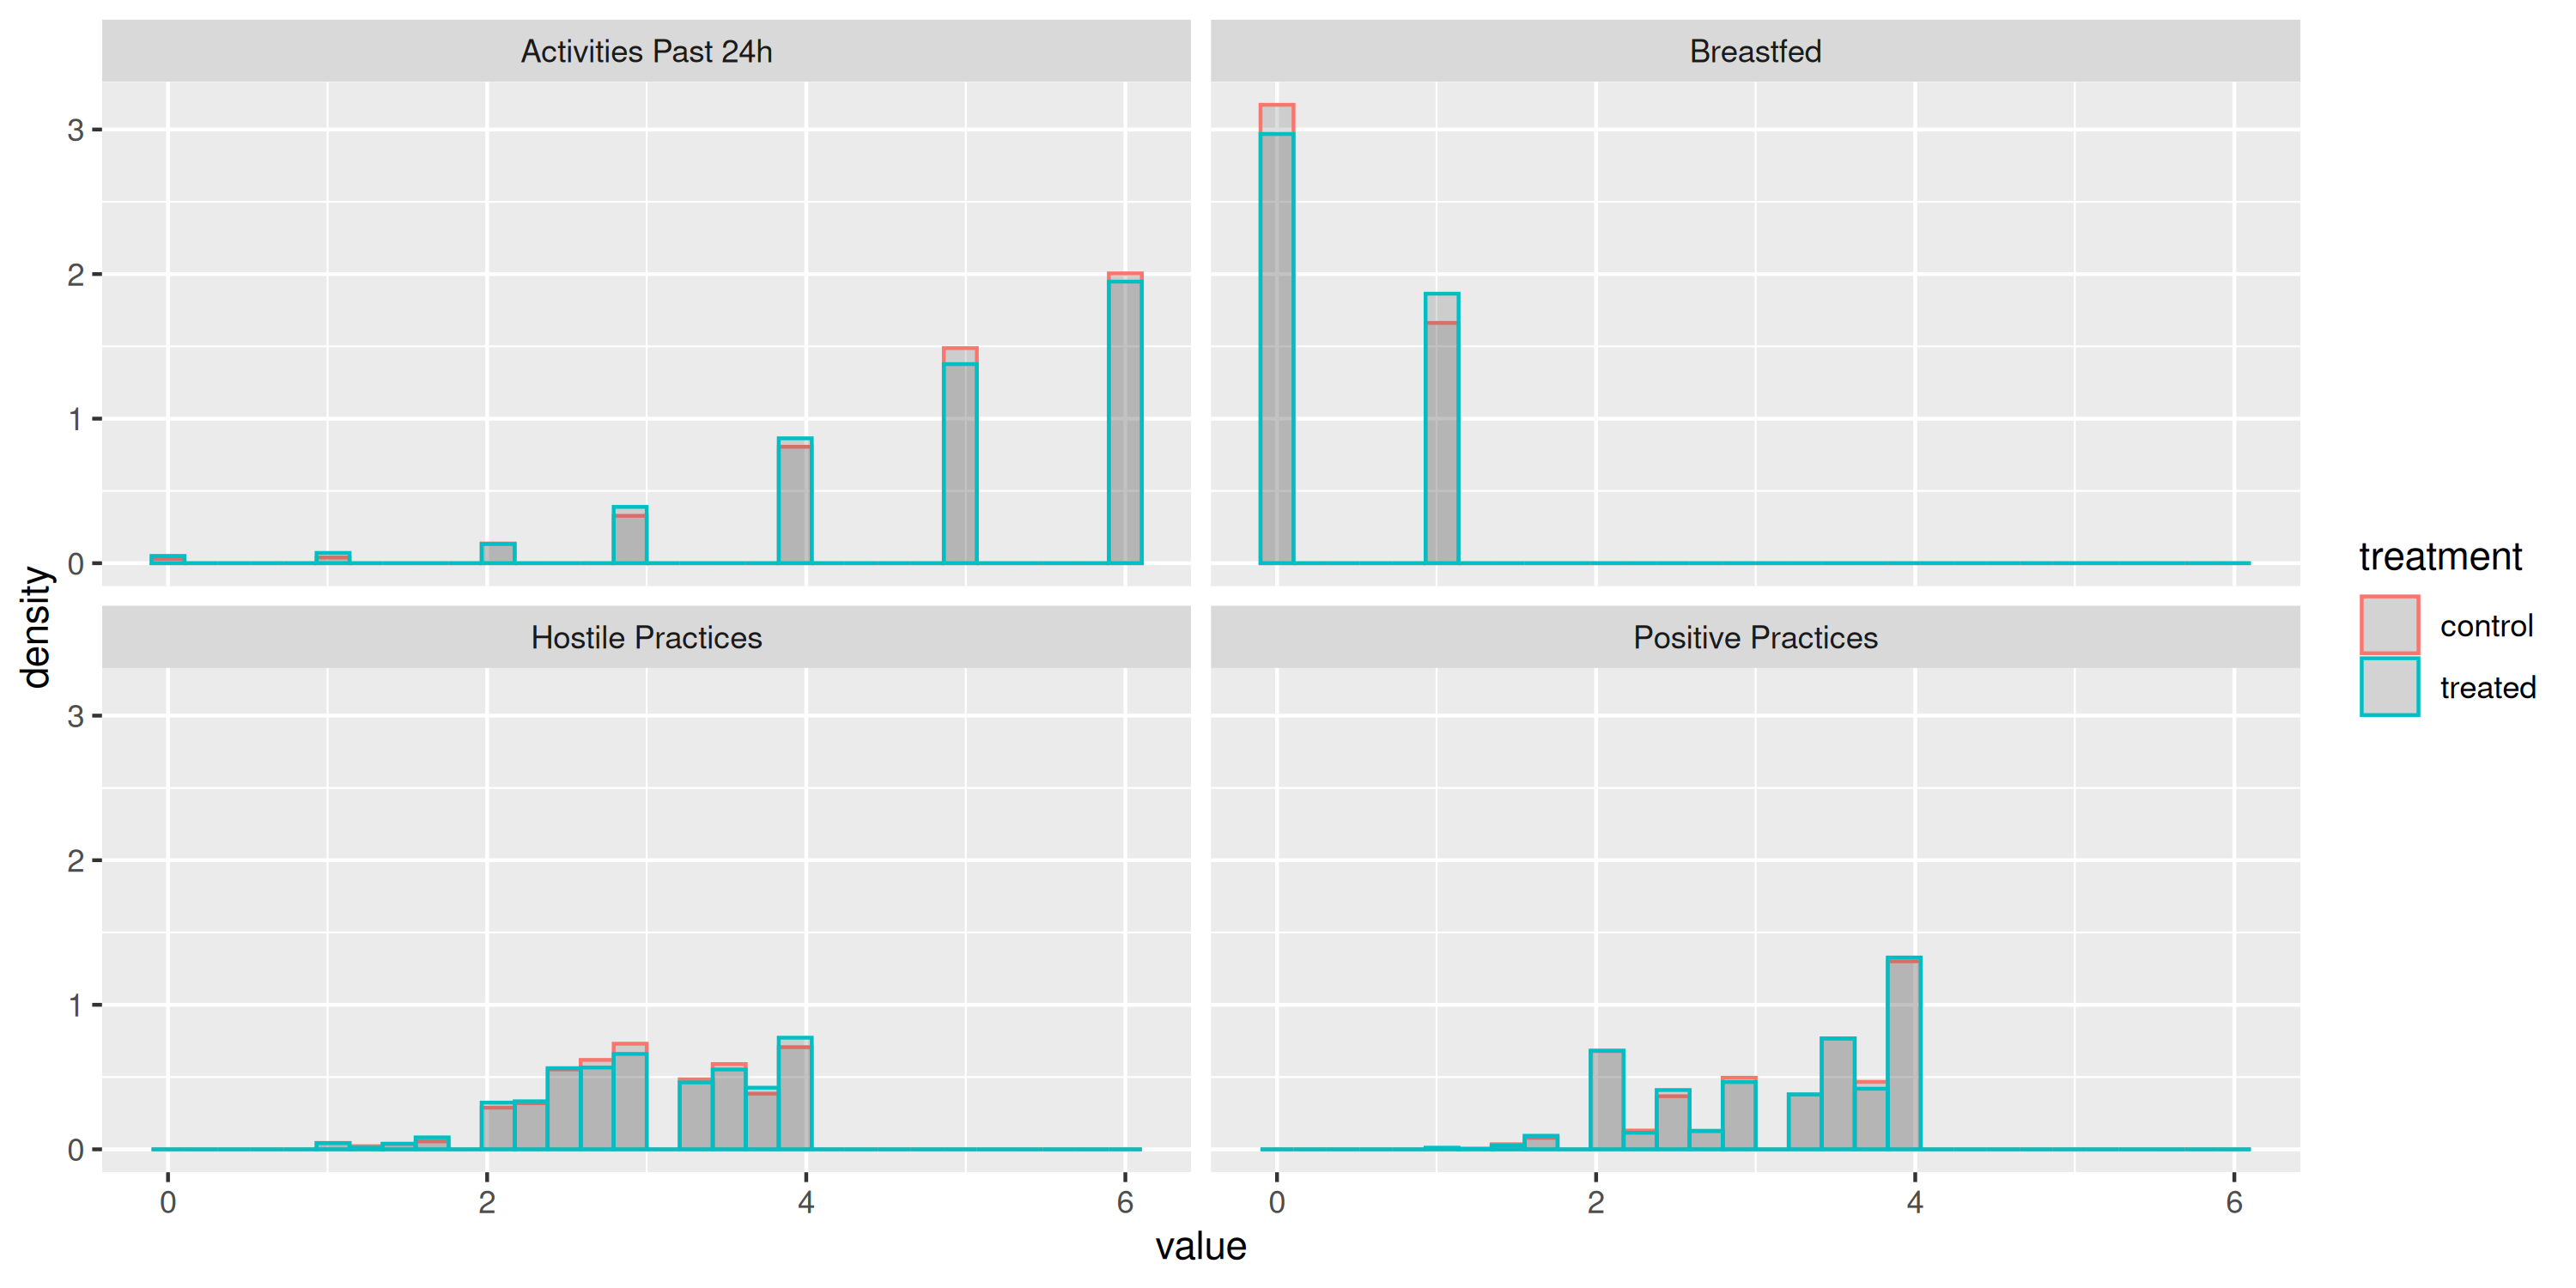
\includegraphics[width=\textwidth]{plots/Original Data - Practices.png}
% 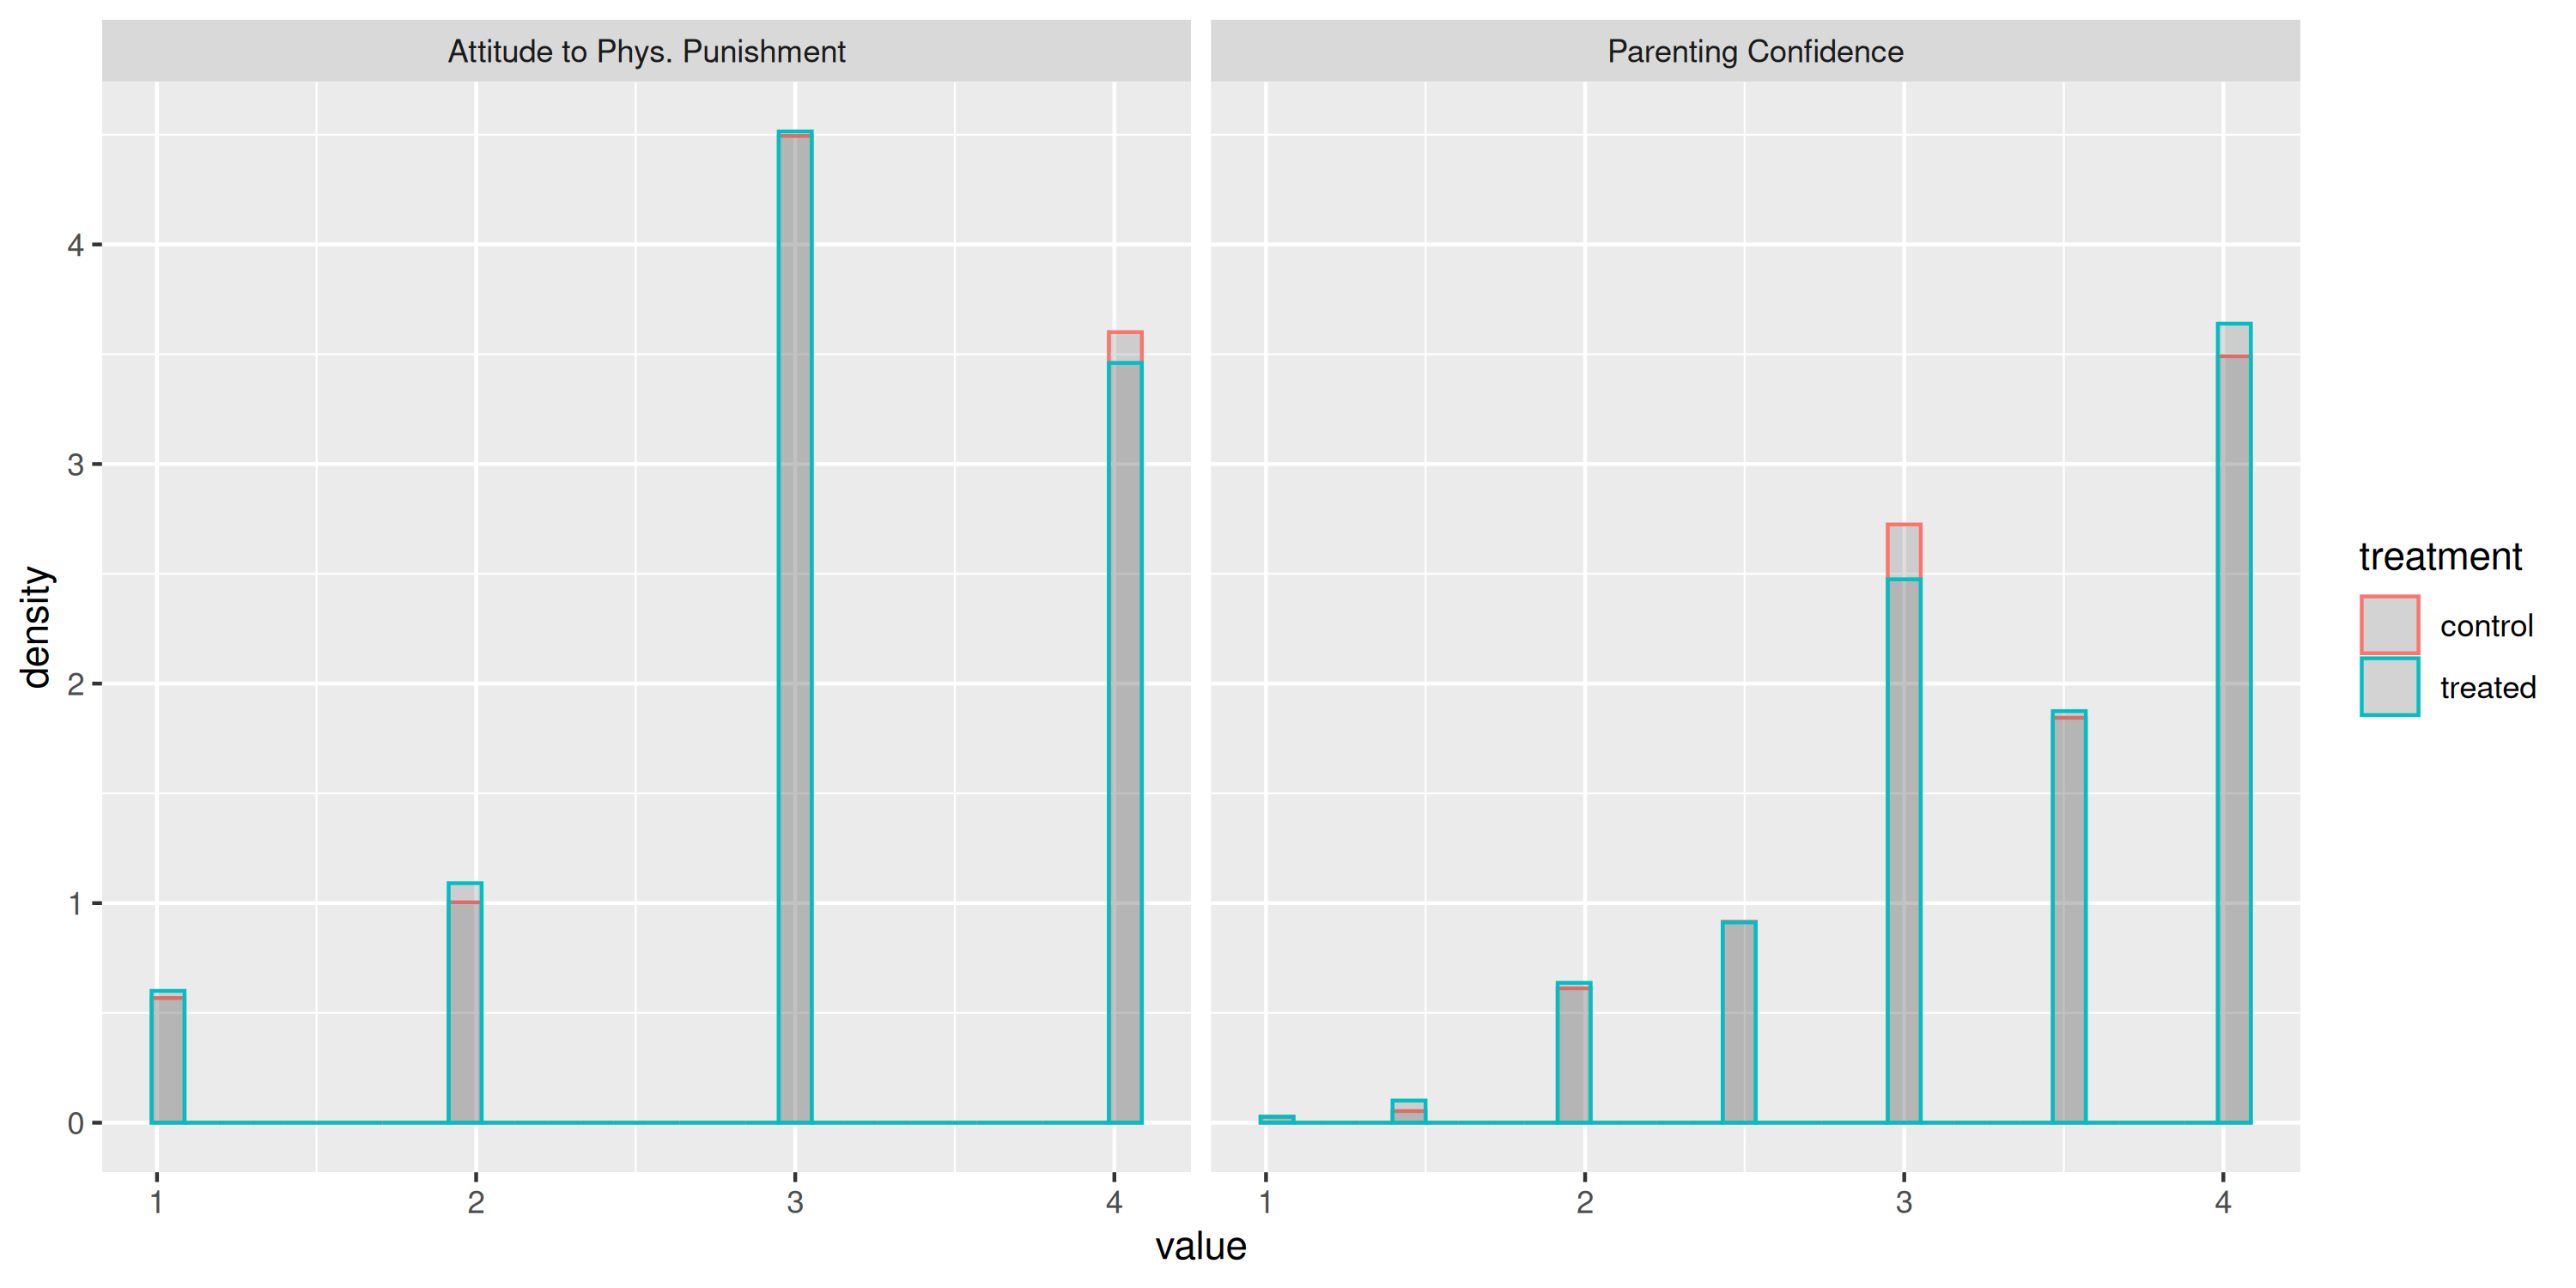
\includegraphics[width=\textwidth]{plots/Original Data - Confidence and Attitudes.png}


% \clearpage

% \section*{Transformed Construct Distributions}
% 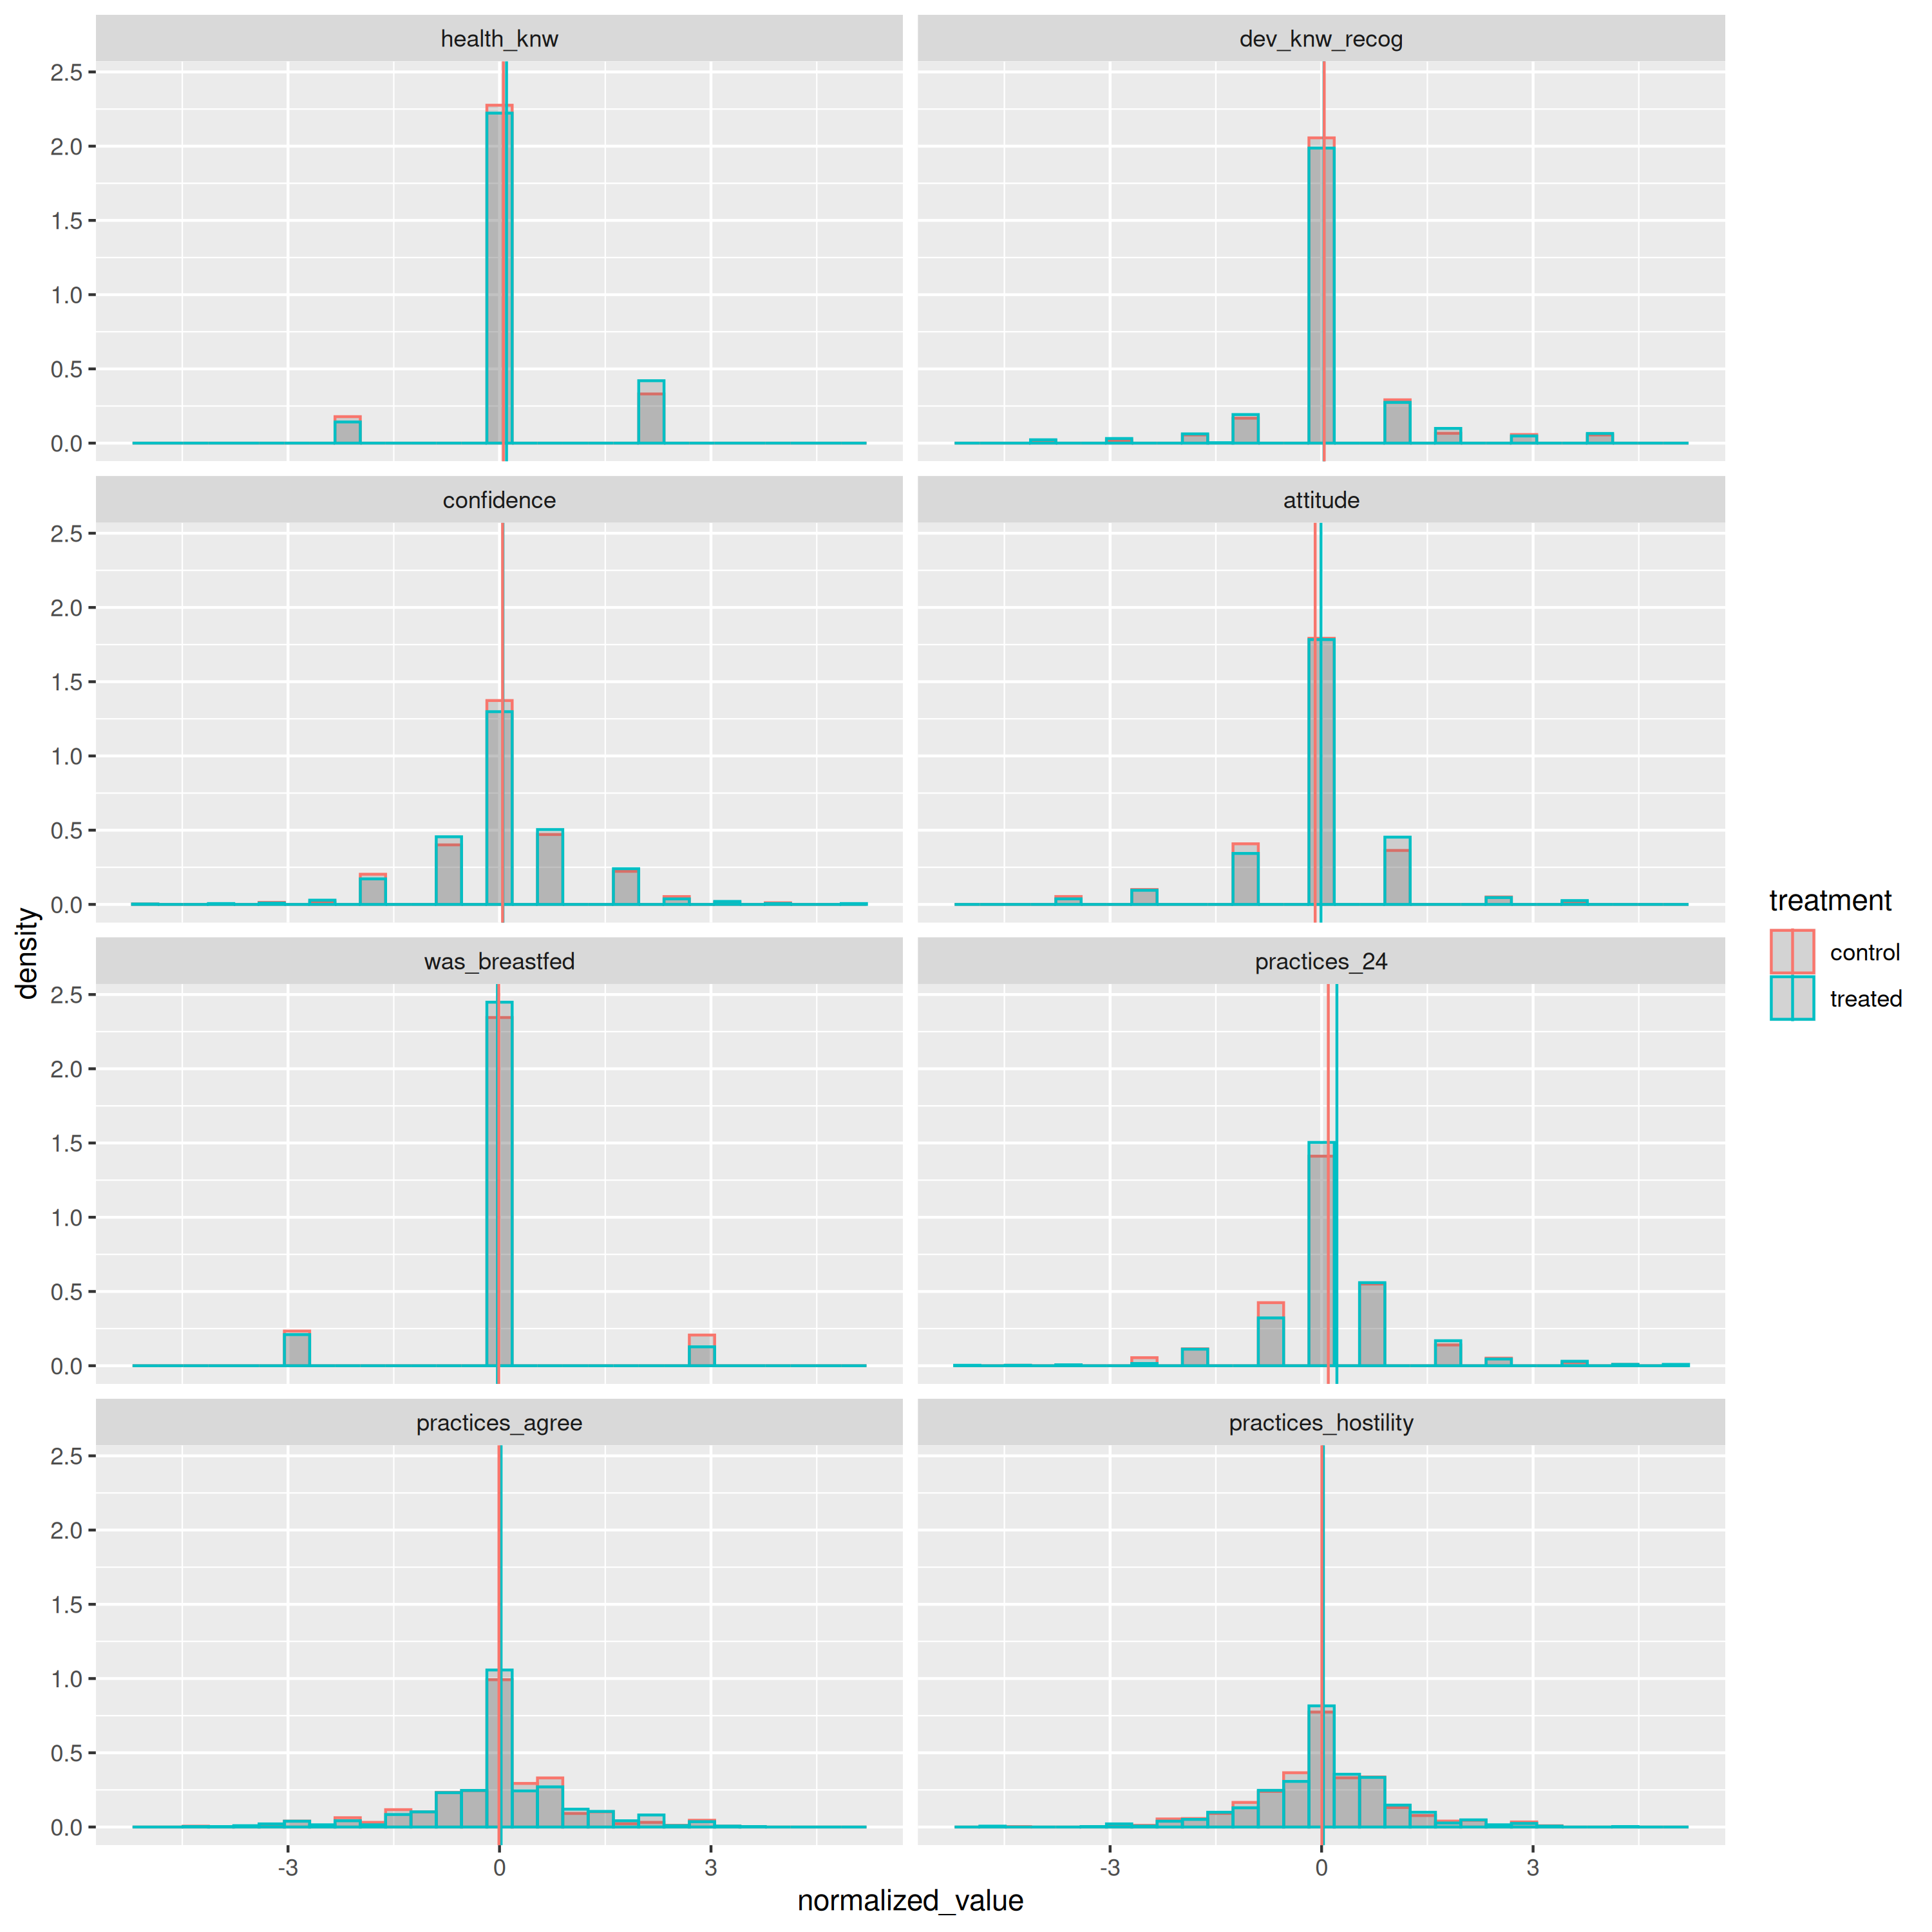
\includegraphics[width=\textwidth]{plots/Transformed Data.png}


% \clearpage


\addcontentsline{toc}{subsection}{Pre-Exposure to Bebbo}
\subsection*{Pre-Exposure to Bebbo}

This study recruited Serbian and Bulgarian caregivers online, via social media ads, and invited half of them to download the app Bebbo. What if some people were already familiar with the app? Or had already downloaded and used it before? This would not impact the internal validity of the study, however, it has implications for the external validity: what it is we are studying exactly.

If someone had already downloaded the app and still had it on their phone, we would not be able to track their usage and they would be considered ``non-compliant'' in this design. This is desireable from an analysis perspective, as these people are ``always-takers'' (\cite{Imbens2015}) who would have the app regardless of whether they were assigned the treatment or control condition.

To check for such ``pre-exposure,'' we ask control group users, at the end of the final follow up survey, if they have ever heard of Bebbo or used Bebbo.

55\% of respondents said that they had heard about the app Bebbo and 23\% said that they had downloaded and used the app Bebbo. It's worth noting that there might be some social desireability bias or acquiesence bias (\cite{Stantcheva2023}) in these responses and we do not have a good way to detect that in this instance. However, despite those potential biases, this is strong suggestive evidence that there was pre-exposure to the treatment in our sample.



\addcontentsline{toc}{subsection}{Power Analysis}
\subsection*{Power Analysis}

Ex-post analysis is provided to show the ability to detect an effect, in terms of standardized deviations (corresponding to Coen's D effect sizes), in the datasets analyzed. To create the effect size, the standardized different is multiplied by the empircal takeup of 28\%, which was the percentage of participants that had at least one learning event in the treatment group. 

The results show that the study is well powered (above 80\%) to detect a medium effect size (0.5 standard deviations) even when that effect is entirely limited to the 28\% takeup group at a significance level of 5\%. We also provide plots showing the power at 1.25\%, to show the equivalent of a 10\% significance level after controlling for multiple testing (8 outcomes) with a Bonferroni correction. See figure \ref{fig:Power Analysis}. 

Thus, the study is well-powered to determine whether or not the 28\% who used the app were impacted.


\addcontentsline{toc}{subsection}{Attrition \& Survey Behavior}
\subsection*{Attrition \& Survey Behavior}

About 52\% of those who started the survey dropped off before completing it and 54\% never came back from the baseline to complete the endline. Table \ref{tbl:Response Rate by Stage} summarizes attrition by stage and treatment condition. It's worth noting that attrition was consistently higher among the treatment group, possibly related to the increased number of questions in the endline survey for that group (additional questions about app usage were added for the treated).

Attrition was particularly high between endline and follow-up survey (66\%) but that includes not only participants who chose not to return for the follow-up, but also those that were disqualified due to an error in survey coding for a portion of early respondents: the questions asked to the control and treatment group was switched at endline, which informed the control group about the existence of the Bebbo app, potentially contaminating them as a pure control. While high pre-existing awareness was discovered in all groups, even those without this mixup, we have removed all cohorts who experienced the mixup from the follow-up survey analysis to avoid any potential issues.


% Table created by stargazer v.5.2.3 by Marek Hlavac, Social Policy Institute. E-mail: marek.hlavac at gmail.com
% Date and time: Mon, Mar 11, 2024 - 09:43:37 PM
\begin{table}[H] \centering 
  \caption{Attrition: Pooled} 
  \label{tbl:Attrition: Pooled} 
\begin{tabular}{@{\extracolsep{5pt}} cccccc} 
\\[-1.8ex]\hline 
\hline \\[-1.8ex] 
stage & count & attrition & treated\_attrition & control\_attrition & attrition\_dif \\ 
\hline \\[-1.8ex] 
Started Baseline & 8994 &  &  &  &  \\ 
Finished Baseline & 4321 & 0.52 & 0.52 & 0.52 & 0.00 \\ 
Started Endline & 1968 & 0.54 & 0.54 & 0.55 & 0.00 \\ 
Finished Endline & 1679 & 0.15 & 0.17 & 0.13 & 0.04 \\ 
Started Followup &  569 & 0.66 & 0.66 & 0.66 & 0.00 \\ 
Finished Followup &  412 & 0.28 & 0.29 & 0.26 & 0.03 \\ 
\hline \\[-1.8ex] 
\end{tabular} 
\end{table} 


Note that respondents should have been contacted 4 weeks after each wave in order to take the subsequent wave. However, two factors may lead to them not always started the wave after exactly 4 weeks: (i) there were some technical issues which caused the notification to be delayed in some cases and (ii) not everyone begins the survey immediately when notified and maybe need to be reminded several times, or may remember on their own, significantly later.

To improve consistency of the study, we removed anyone who took the endline or followup surveys more than 9 weeks after their previous survey, ensuring that all respondents were responding in a gap between 4-9 weeks. Table \ref{tbl:Time Gap Descriptives} summarizes the distribution of this time gap. As you can see, the vast majority (more than 80\%) took the survey after 4-5 weeks of the previous survey.


% Table created by stargazer v.5.2.3 by Marek Hlavac, Social Policy Institute. E-mail: marek.hlavac at gmail.com
% Date and time: Mon, Mar 18, 2024 - 11:41:42 PM
\begin{table}[!htbp] \centering 
  \caption{Time Gap Descriptives} 
  \label{tbl:Time Gap Descriptives} 
\begin{tabular}{@{\extracolsep{5pt}} cccccc} 
\\[-1.8ex]\hline 
\hline \\[-1.8ex] 
min & quantile\_05 & median & quantile\_95 & max & Time Gap \\ 
\hline \\[-1.8ex] 
 2 days & 28 days & 29 days & 57 days & 277 days & Baseline - Endline \\ 
28 days & 28 days & 29 days & 51 days & 173 days & Endline - Followup \\ 
\hline \\[-1.8ex] 
\end{tabular} 
\end{table} 


\addcontentsline{toc}{subsection}{App Usage Characteristics}
\subsection*{App Usage Characteristics}

To measure takeup, we pick how many distinct days the participant used the app, as measured by one of the predefined set of ``learning events'' that include looking at material or entering milestones for their child. Note that in order to generate a ``learning event,'' one must get past the ``welcome'' screens and create a profile for their child.

Figure \ref{fig:treatment-takeup-histogram} shows a histogram of the amount of days that respondents in the treatment group used the Bebbo app. Table \ref{tbl:Treatment Takeup} shows some takeup numbers for different intensities of usage. Very few treated respondents used the app more than three days (less than 3\%) and only about 12\% used it more than once. The maximum group of 8 people, less than 1\% of the population treated, used the app on more than 5 days in the 4-6 week period.

Additionally, table \ref{tbl:App Retention Funnel} shows a retention funnel for those that did download the app, including data from app usage in Serbia and Bulgaria that was not associated with the study. Note that, of those who did download the app in the study (and therefore were complying with the reccomendations of the study) only about 55\% actually finished creating a profile for their child and only 24\% used the app past the first day and 5\% used it for more than 3 days.

The numbers are worse for those outside of the study. Note that these numbers were restricted to 30 days after downloading, to compare with the timeframe between baseline and endline within the study. These numbers show that only 28.5\% of downloaders actually complete a profile and access content and only 14.9\% of downloaders access learning content more than one day. These are important results. 75-85\% of downloaders churning after the first day indicates that the app is not engaging or attractive to the majority of caregivers of young children who agree to download it. This is true both in our study population as well as for those who download the app in the wild.


\begin{figure}[H]
  \centering
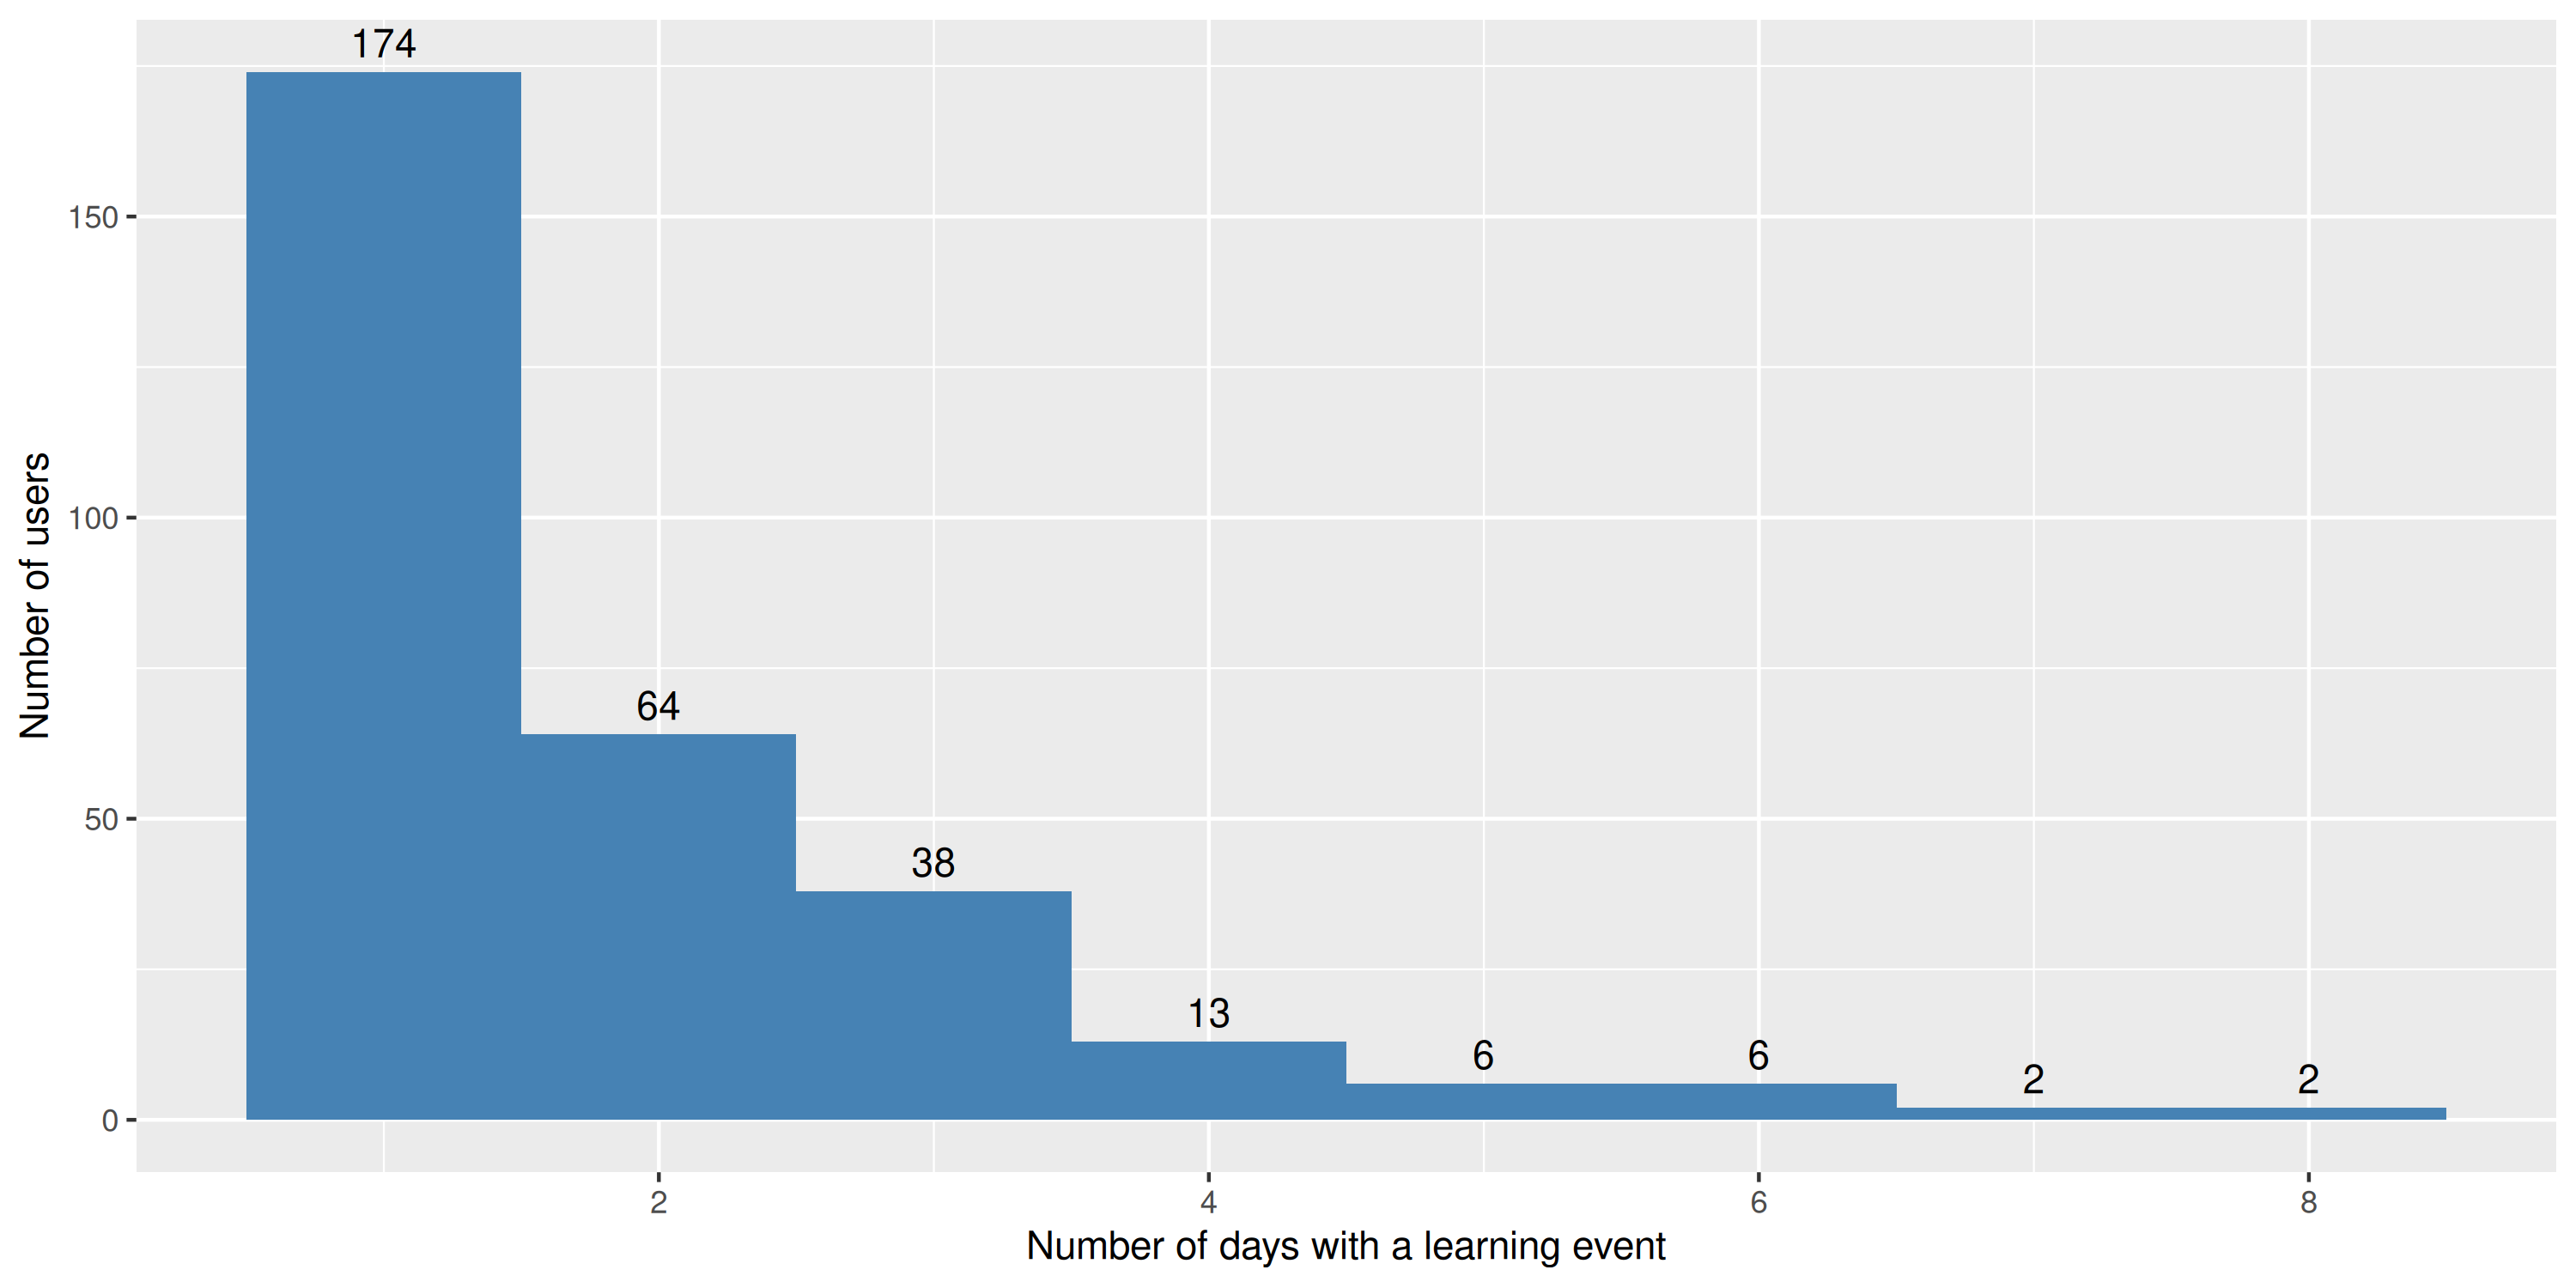
\includegraphics[width=\textwidth]{plots/Treatment Takeup Baseline - Endline.png}
\caption{Days with Learning Event (Baseline - Endline)}
\label{fig:treatment-takeup-histogram}
\end{figure}



% Table created by stargazer v.5.2.3 by Marek Hlavac, Social Policy Institute. E-mail: marek.hlavac at gmail.com
% Date and time: Wed, Mar 20, 2024 - 10:37:13 PM
\begin{table}[H] \centering 
  \caption{Treatment Takeup} 
  \label{tbl:Treatment Takeup} 
\begin{tabular}{@{\extracolsep{5pt}} ccccccccc} 
\\[-1.8ex]\hline 
\hline \\[-1.8ex] 
Dataset & Treated & Downloaded & Used & \textgreater  1 Day & \textgreater  3 Days & Used (\%) & \textgreater  1 Day (\%) & \textgreater  3 Days (\%) \\ 
\hline \\[-1.8ex] 
Serbia &  678 & 379 & 189 &  85 & 18 & 27.9\% & 12.5\% & 2.7\% \\ 
Bulgaria &  342 & 182 & 116 &  46 & 11 & 33.9\% & 13.5\% & 3.2\% \\ 
Pooled & 1020 & 561 & 305 & 131 & 29 & 29.9\% & 12.8\% & 2.8\% \\ 
\hline \\[-1.8ex] 
\end{tabular} 
\end{table} 



% Table created by stargazer v.5.2.3 by Marek Hlavac, Social Policy Institute. E-mail: marek.hlavac at gmail.com
% Date and time: Sun, Feb 25, 2024 - 11:50:08 PM
\begin{table}[H] \centering 
  \caption{App Retention Funnel} 
  \label{tbl:App Retention Funnel} 
\begin{tabular}{@{\extracolsep{5pt}} ccccc} 
\\[-1.8ex]\hline 
\hline \\[-1.8ex] 
Dataset & Downloaded & Used (\%) & \textgreater  1 Day (\%) & \textgreater  3 Days (\%) \\ 
\hline \\[-1.8ex] 
Serbia & 340 & 0.503 & 0.226 & 0.044 \\ 
Bulgaria & 162 & 0.642 & 0.253 & 0.062 \\ 
Pooled & 497 & 0.547 & 0.237 & 0.050 \\ 
\hline \\[-1.8ex] 
\end{tabular} 
\end{table} 



\section{Results}

\addcontentsline{toc}{subsection}{Regression Model}
\subsection*{Regression Model}

We run the following regression model to measure the intent-to-treat effect (ITT) of assignment to the treatment arm:
$$
y_{i} - y^{b}_i = \gamma_1 + \beta T_{i} + \gamma_2X_{i} + \epsilon_i
$$

Where $y_i$ represents the outcome of interest for individual $i$ measured after treatment, $T_i$ represents the random treatment assignment, $X_i$ a set of control variables and $y^b_i$ represents the outcome of interest measured before treatment. The parameter of interest will be the treatment effect, $\beta$.

Note that due to the relatively large number of sepearate outcomes (8), we adjust p-values of the treatment variable to control the false discovery rate (FDR), using Benjamini-Hochberg, reported as the ``Adjusted Treatment p-value.''

Of interest in this analysis is also the treatment effect on the treated (ToT), which can be estimated using an instrumental variable model given the monotonicity assumption of treatment (\cite{Imbens2015}), which assumes that people are not less likely to download and use the Bebbo app in the treatment group. To estimate our instrumental variable model, we use 2-stage least squares:
\begin{align*}
y_{i} - y^{b}_i &= \gamma_1 + \beta \hat{z}_{i} + \gamma_2X_{i} + \epsilon_i \\
z_{i} &= \gamma_3 + \gamma_4 T_{i} + \gamma_5X_{i} + \delta_i
\end{align*}

Where $z_i$ is a binary indicator of takeup based on the recorded app-usage data and $\hat{z_i}$ the predicted takeup based on the first stage regression. Once again, parameter of interest is $\beta$. It's worth noting that, given that we cannot say we measured any impact (results are not significant from zero) in the ITT model, the exact values of the ToT model are of less interest and the associated tables can be found in the appendix.

We also run the regression for two separate time periods: endline and follow-up. However, due to large attrition in the follow-up survey and the low long-term app takeup, the decision was made to rescope this evaluation to focus on the endline. Additional tables are available in the appendix.

One of the dangers of a prepost design is that you are priming your respondents with the first survey and that priming may impact how they answer the questions in the post-treatment survey(s) (\cite{Stantcheva2023}). Given this particular study design, where our control is a ``treatment as usual'' (TAU) that involved sharing a website and we do not have data regarding the takeup, or usage, of the website, it is difficult to isolate a priming effect.

We will also plot raw charts showing mean scores at baseline and endline for three groups for each variable: control, treatment with takeup (those who we know downloaded and used the app), treatment without takeup (those for whom we have no data showing they downloaded or used the app). These plots can provide suggestive evidence of priming effects by showing the shift in mean between baseline and endline across all three groups.

Table \ref{tbl:Baseline Respondent Characteristics}, with the baseline respondent characteristics, shows all the control variables used. Note that several outcomes only applied to parents with children in a certain age group: "Breastfed" and "Vaccine Knowledge" applied to those with children ages 0-2. Thus, the binary control variable representing the age of the child (0-2 or 2-6) was removed in those regressions.

\addcontentsline{toc}{subsection}{Knowledge and Awareness}
\subsection*{Knowledge and Awareness}

Regression analysis of these outcome constructs show no significant result of treatment:


% Table created by stargazer v.5.2.3 by Marek Hlavac, Social Policy Institute. E-mail: marek.hlavac at gmail.com
% Date and time: Sun, Feb 11, 2024 - 04:03:43 PM
\begin{table}[!htbp] \centering 
  \caption{Pooled: OLS - Endline - Knowledge and Awareness} 
  \label{tbl:Pooled: OLS - Endline - Knowledge and Awareness} 
\begin{tabular}{@{\extracolsep{5pt}}lcc} 
\\[-1.8ex]\hline 
\hline \\[-1.8ex] 
 & \multicolumn{2}{c}{\textit{Dependent variable:}} \\ 
\cline{2-3} 
\\[-1.8ex] & Vaccine Knowledge & Child Dev. Knowledge \\ 
\\[-1.8ex] & (1) & (2)\\ 
\hline \\[-1.8ex] 
 Treatment & 0.04 & $-$0.001 \\ 
  & (0.03) & (0.01) \\ 
  & & \\ 
\hline \\[-1.8ex] 
Adjusted Treatment p-value & 0.467 & 0.957 \\ 
Observations & 667 & 1,811 \\ 
R$^{2}$ & 0.01 & 0.01 \\ 
\hline 
\hline \\[-1.8ex] 
\textit{Note:}  & \multicolumn{2}{r}{$^{*}$p$<$0.1; $^{**}$p$<$0.05; $^{***}$p$<$0.01} \\ 
\end{tabular} 
\end{table} 


These two constructs, Vaccine Knowledge and Child Development Knowledge, both suffered from ceiling effects in the baseline survey (72\% and 73\% respectively). On top of those ceiling effets, they both potentially suffered from priming effects, as evidenced by the consistent improvement in the endline survey for all groups.

Note that there is some suggestive evidence that those with less vaccine knowledge were more likely to download the app, indicating that takeup might be biased towards those who need it the most. That might be driving the small and statistically insignificant positive measured impact on Vaccine Knowledge in the regression. Unfortunately, the study was not designed for subgroup analysis on a small group such as the 28\% who failed the vaccine knowledge question at baseline.
\begin{figure}[H]
  \centering
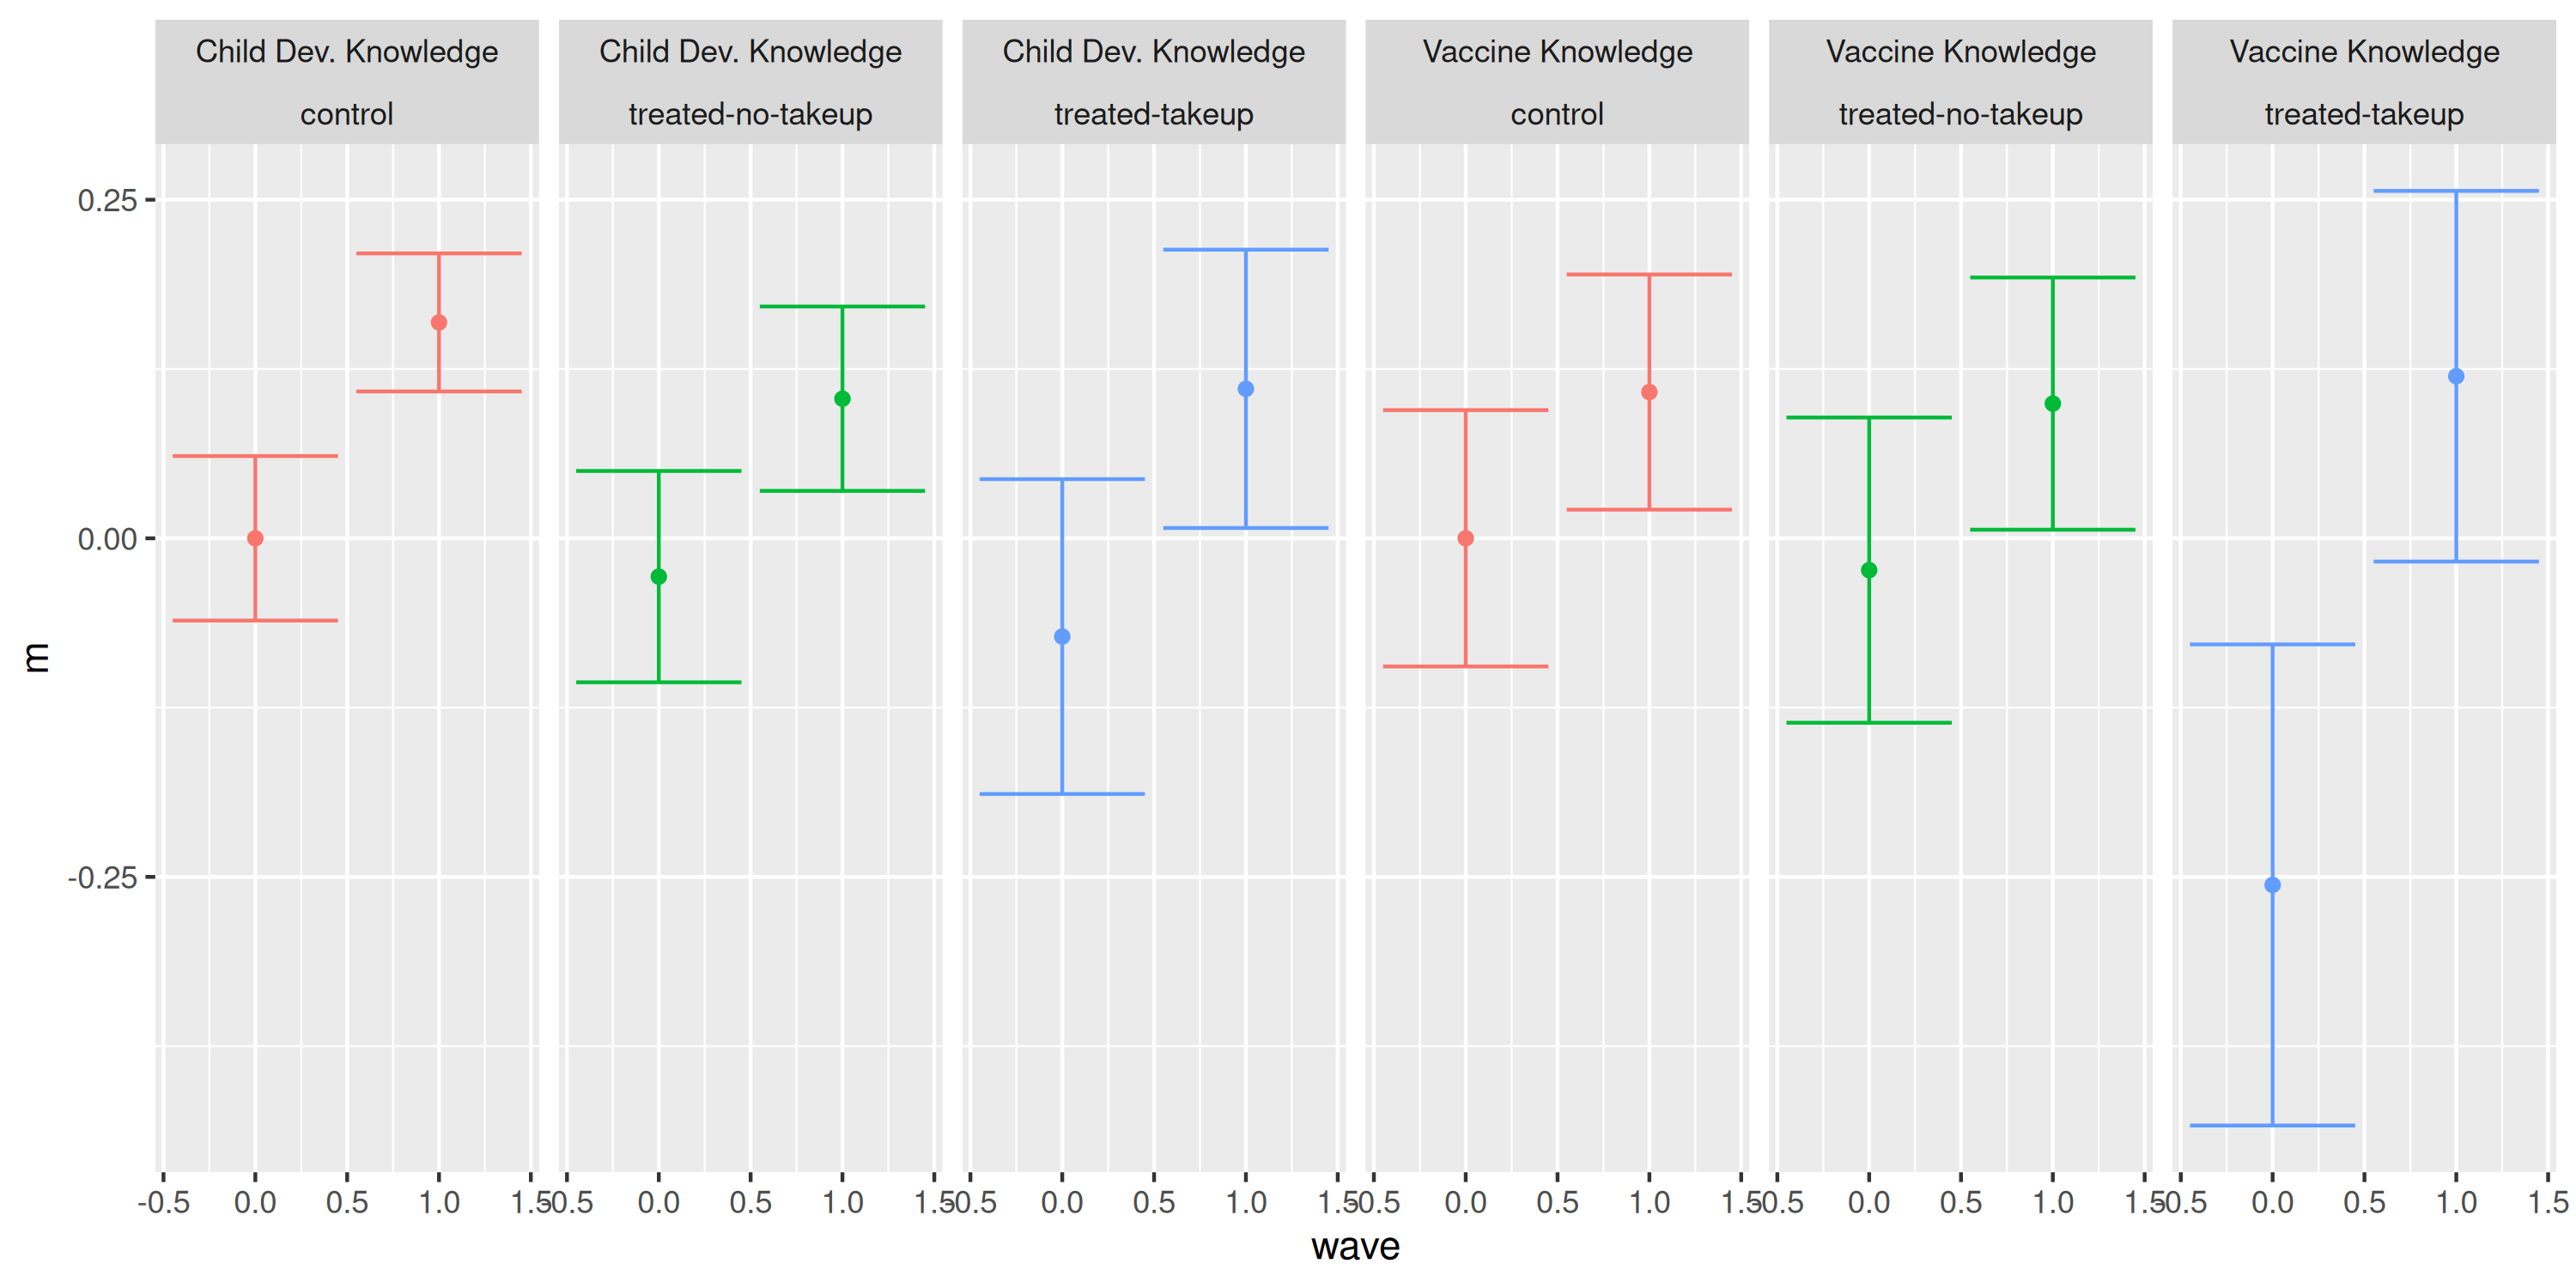
\includegraphics[width=\textwidth]{plots/pre_post/Pooled: Vaccine Knowledge.png}
\end{figure}


\addcontentsline{toc}{subsection}{Confidence and Attitudes}
\subsection*{Confidence and Attitudes}

Attitude Towards Physical punishment is a single question which asks if the parent believes the child needs to be physically punished. While there might seem to be some suggestive evidence from the coefficients of the regression model, the raw data shows that the positive coefficient is indicative of the fact that the control group got worse over time! They were more supportive of phyisical punishment in the endline survey. While there might be a story to that, it could also be the exact kind of statistical anomaly that multiple testing correction is designed to help us avoid when checking so many outcomes.

Parenting Confidence shows no significant impact in the regression analysis. The raw data shows suggestive evidence that those with lower confidence might be more likely to take up the treatment. The lack of a positive coefficient in the regression, however, might indicate that those in the control group were equally likely to take up either the control website or seek out information on their own in order to improve by endline.


% Table created by stargazer v.5.2.3 by Marek Hlavac, Social Policy Institute. E-mail: marek.hlavac at gmail.com
% Date and time: Sun, Jan 21, 2024 - 11:01:29 PM
\begin{table}[!htbp] \centering 
  \caption{Pooled: OLS - Endline - Confidence and Attitudes} 
  \label{tbl:Pooled: OLS - Endline - Confidence and Attitudes} 
\begin{tabular}{@{\extracolsep{5pt}}lcc} 
\\[-1.8ex]\hline 
\hline \\[-1.8ex] 
 & \multicolumn{2}{c}{\textit{Dependent variable:}} \\ 
\cline{2-3} 
\\[-1.8ex] & Parenting Confidence & Attitude to Phys. Punishment \\ 
\\[-1.8ex] & (1) & (2)\\ 
\hline \\[-1.8ex] 
 Treatment & $-$0.02 & 0.08 \\ 
  & (0.03) & (0.04) \\ 
  & & \\ 
\hline \\[-1.8ex] 
Adjusted Treatment p-value & 0.695 & 0.133 \\ 
Observations & 1,905 & 1,892 \\ 
R$^{2}$ & 0.003 & 0.01 \\ 
\hline 
\hline \\[-1.8ex] 
\textit{Note:}  & \multicolumn{2}{r}{$^{*}$p$<$0.1; $^{**}$p$<$0.05; $^{***}$p$<$0.01} \\ 
\end{tabular} 
\end{table} 

\begin{figure}[H]
  \centering
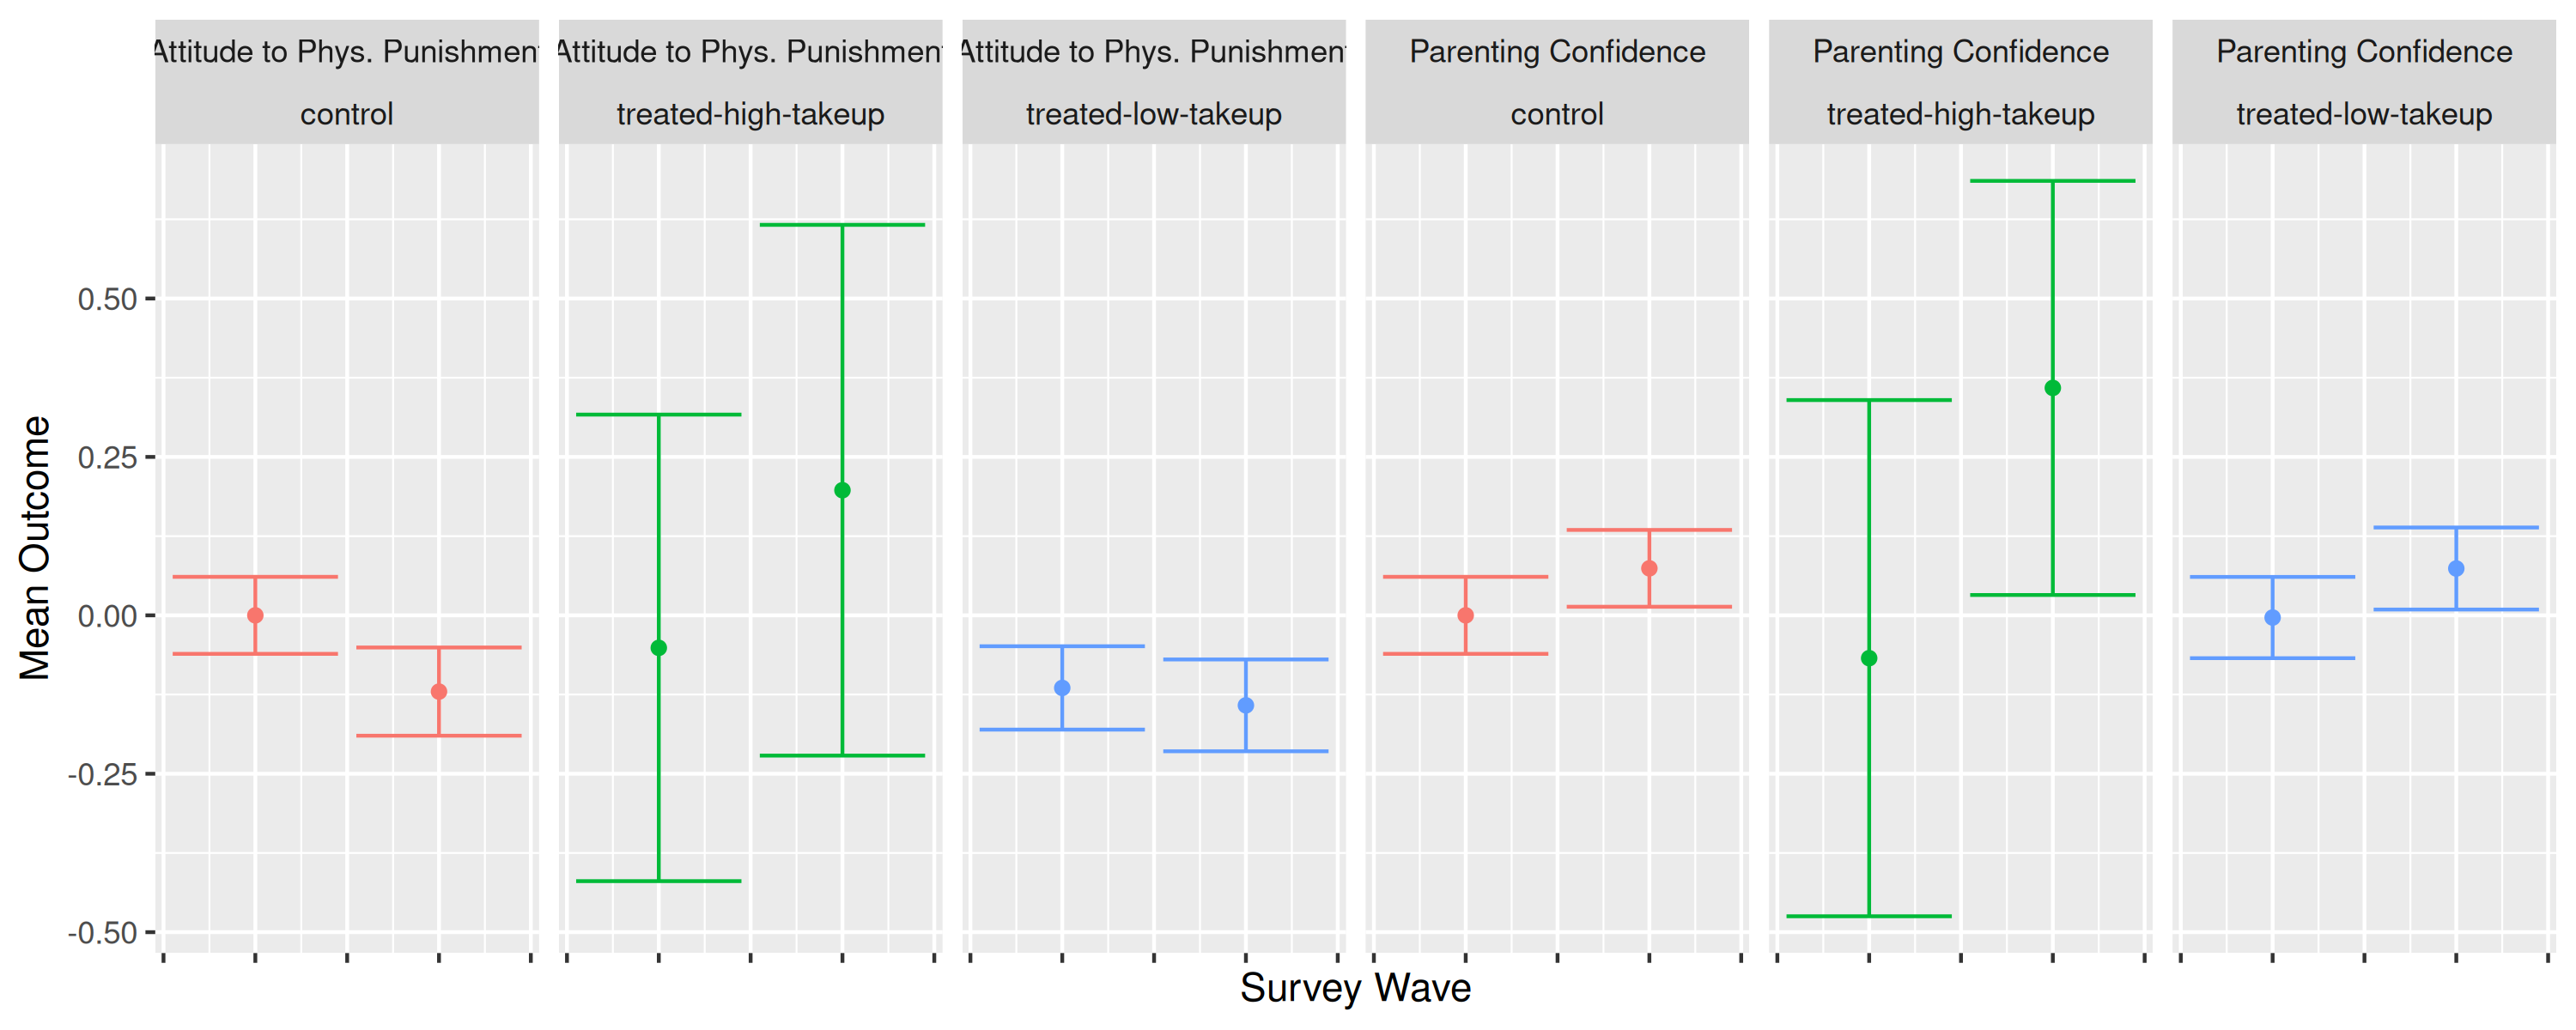
\includegraphics[width=\textwidth]{plots/pre_post/Pooled: Parenting Confidence.png}
\end{figure}


\addcontentsline{toc}{subsection}{Practices}
\subsection*{Practices}

These four constructs all relate to practices and behaviors of the parent. No significant effect was found for any of the behaviors and there is not much suggestive evidence of selective takeup either. The raw regression results suggest that Activities Past 24h show suggestive evidence of impact, but the raw data shows that the much of the improvement is driven by those in the treated group who did not takeup the treatment, which gives credence to the assumption that this could be statistical noise and is why we have corrected for multiple testing.


% Table created by stargazer v.5.2.3 by Marek Hlavac, Social Policy Institute. E-mail: marek.hlavac at gmail.com
% Date and time: Wed, Jan 24, 2024 - 09:15:00 PM
\begin{table}[!htbp] \centering 
  \caption{Pooled: OLS - Endline - Practices} 
  \label{tbl:Pooled: OLS - Endline - Practices} 
\begin{tabular}{@{\extracolsep{5pt}}lcccc} 
\\[-1.8ex]\hline 
\hline \\[-1.8ex] 
 & \multicolumn{4}{c}{\textit{Dependent variable:}} \\ 
\cline{2-5} 
\\[-1.8ex] & Breastfed & Activities Past 24h & Positive Practices & Hostile Practices \\ 
\\[-1.8ex] & (1) & (2) & (3) & (4)\\ 
\hline \\[-1.8ex] 
 Treatment & $-$0.02 & 0.12 & 0.02 & 0.02 \\ 
  & (0.03) & (0.05) & (0.03) & (0.03) \\ 
  & & & & \\ 
\hline \\[-1.8ex] 
Adjusted Treatment p-value & 0.695 & 0.133 & 0.695 & 0.695 \\ 
Observations & 657 & 1,832 & 1,832 & 1,827 \\ 
R$^{2}$ & 0.02 & 0.01 & 0.01 & 0.01 \\ 
\hline 
\hline \\[-1.8ex] 
\textit{Note:}  & \multicolumn{4}{r}{$^{*}$p$<$0.1; $^{**}$p$<$0.05; $^{***}$p$<$0.01} \\ 
\end{tabular} 
\end{table} 


\begin{figure}[H]
  \centering
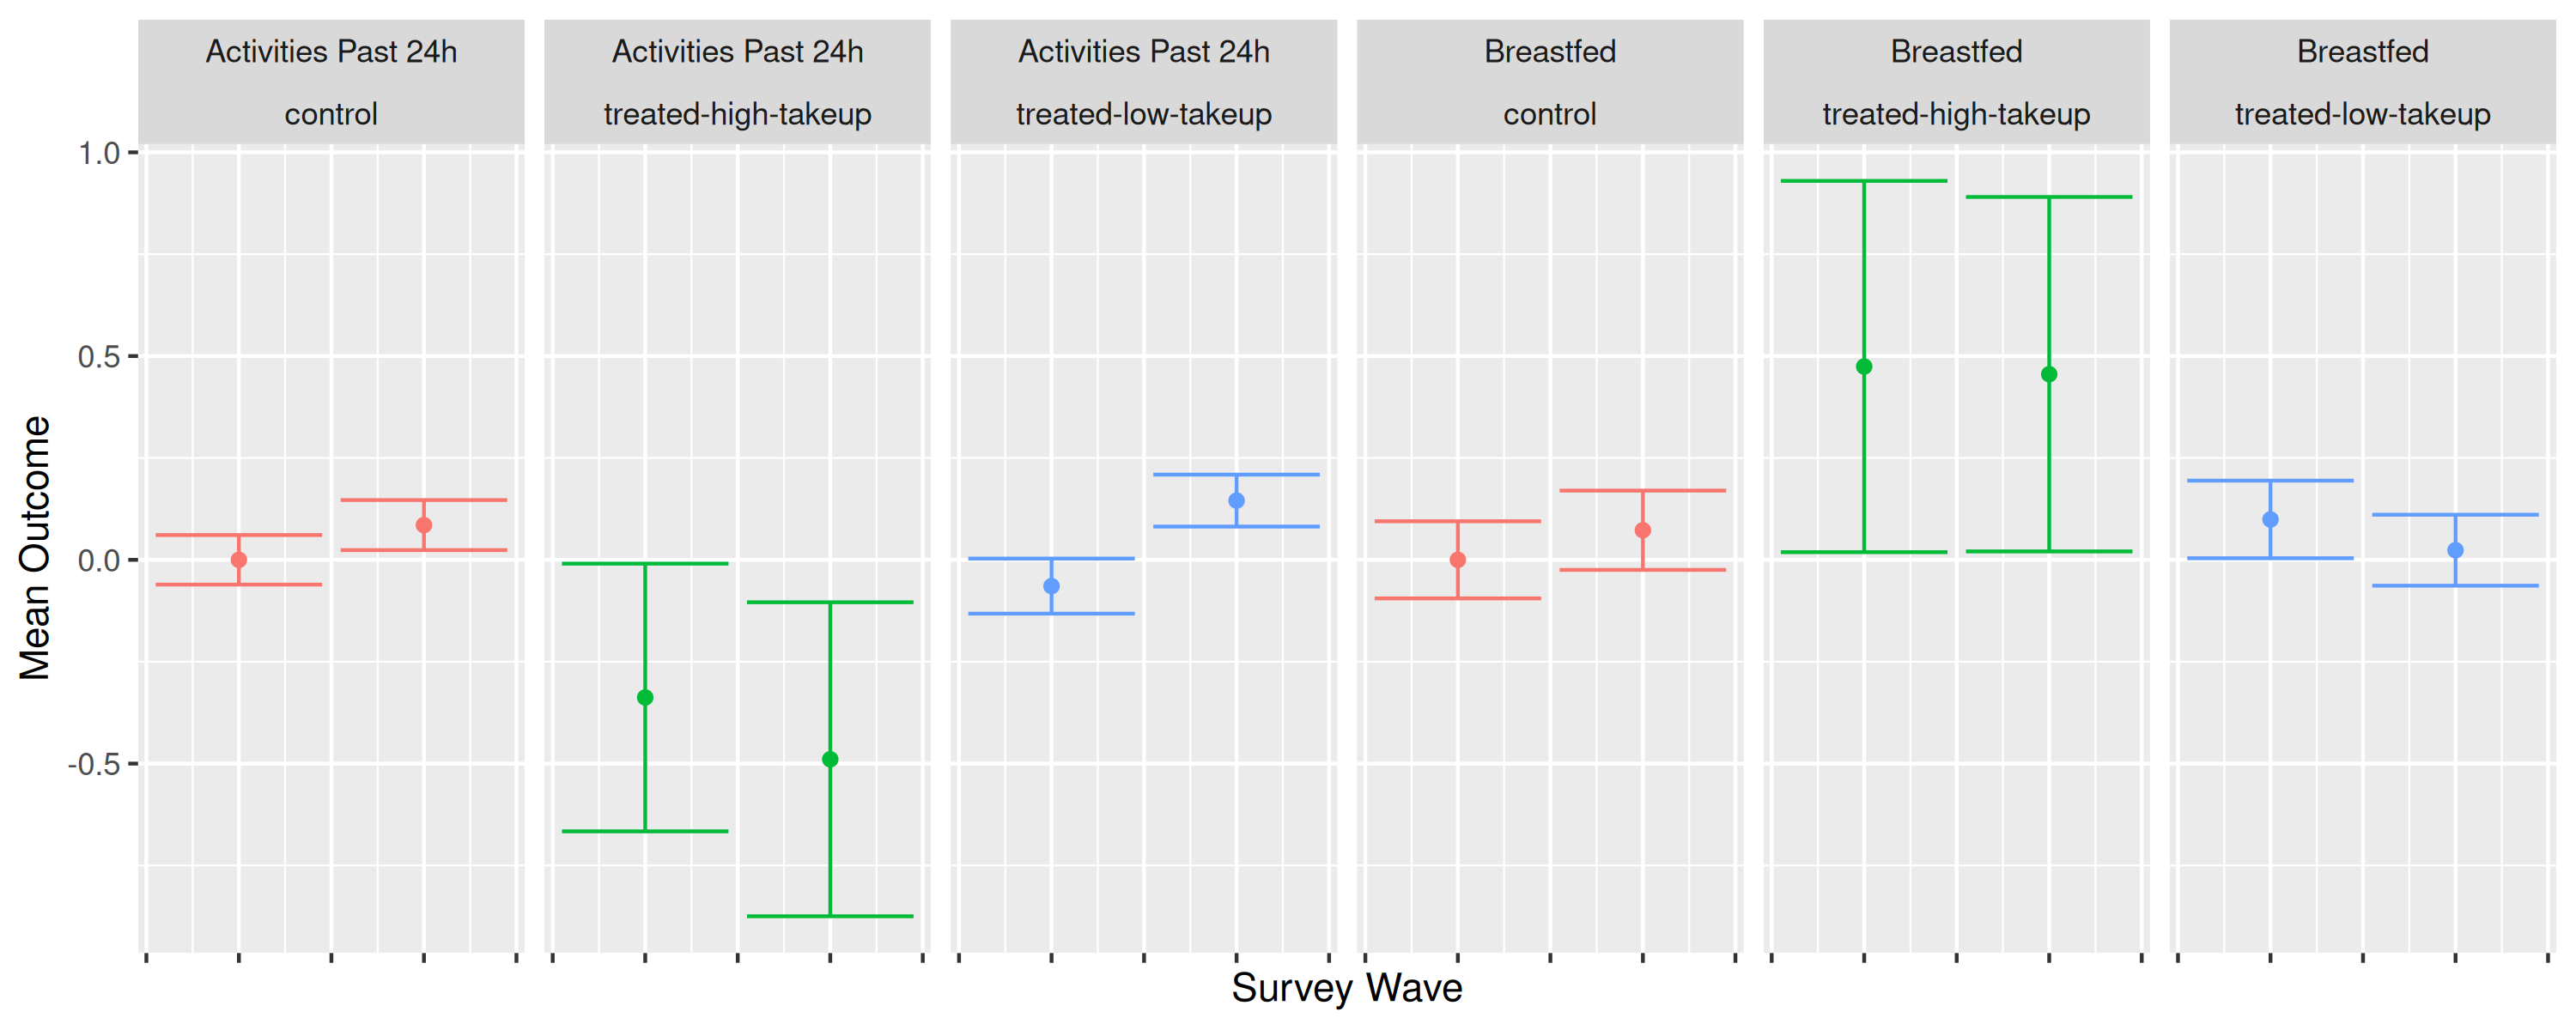
\includegraphics[width=0.9\textwidth]{plots/pre_post/Pooled: Breastfed.png}
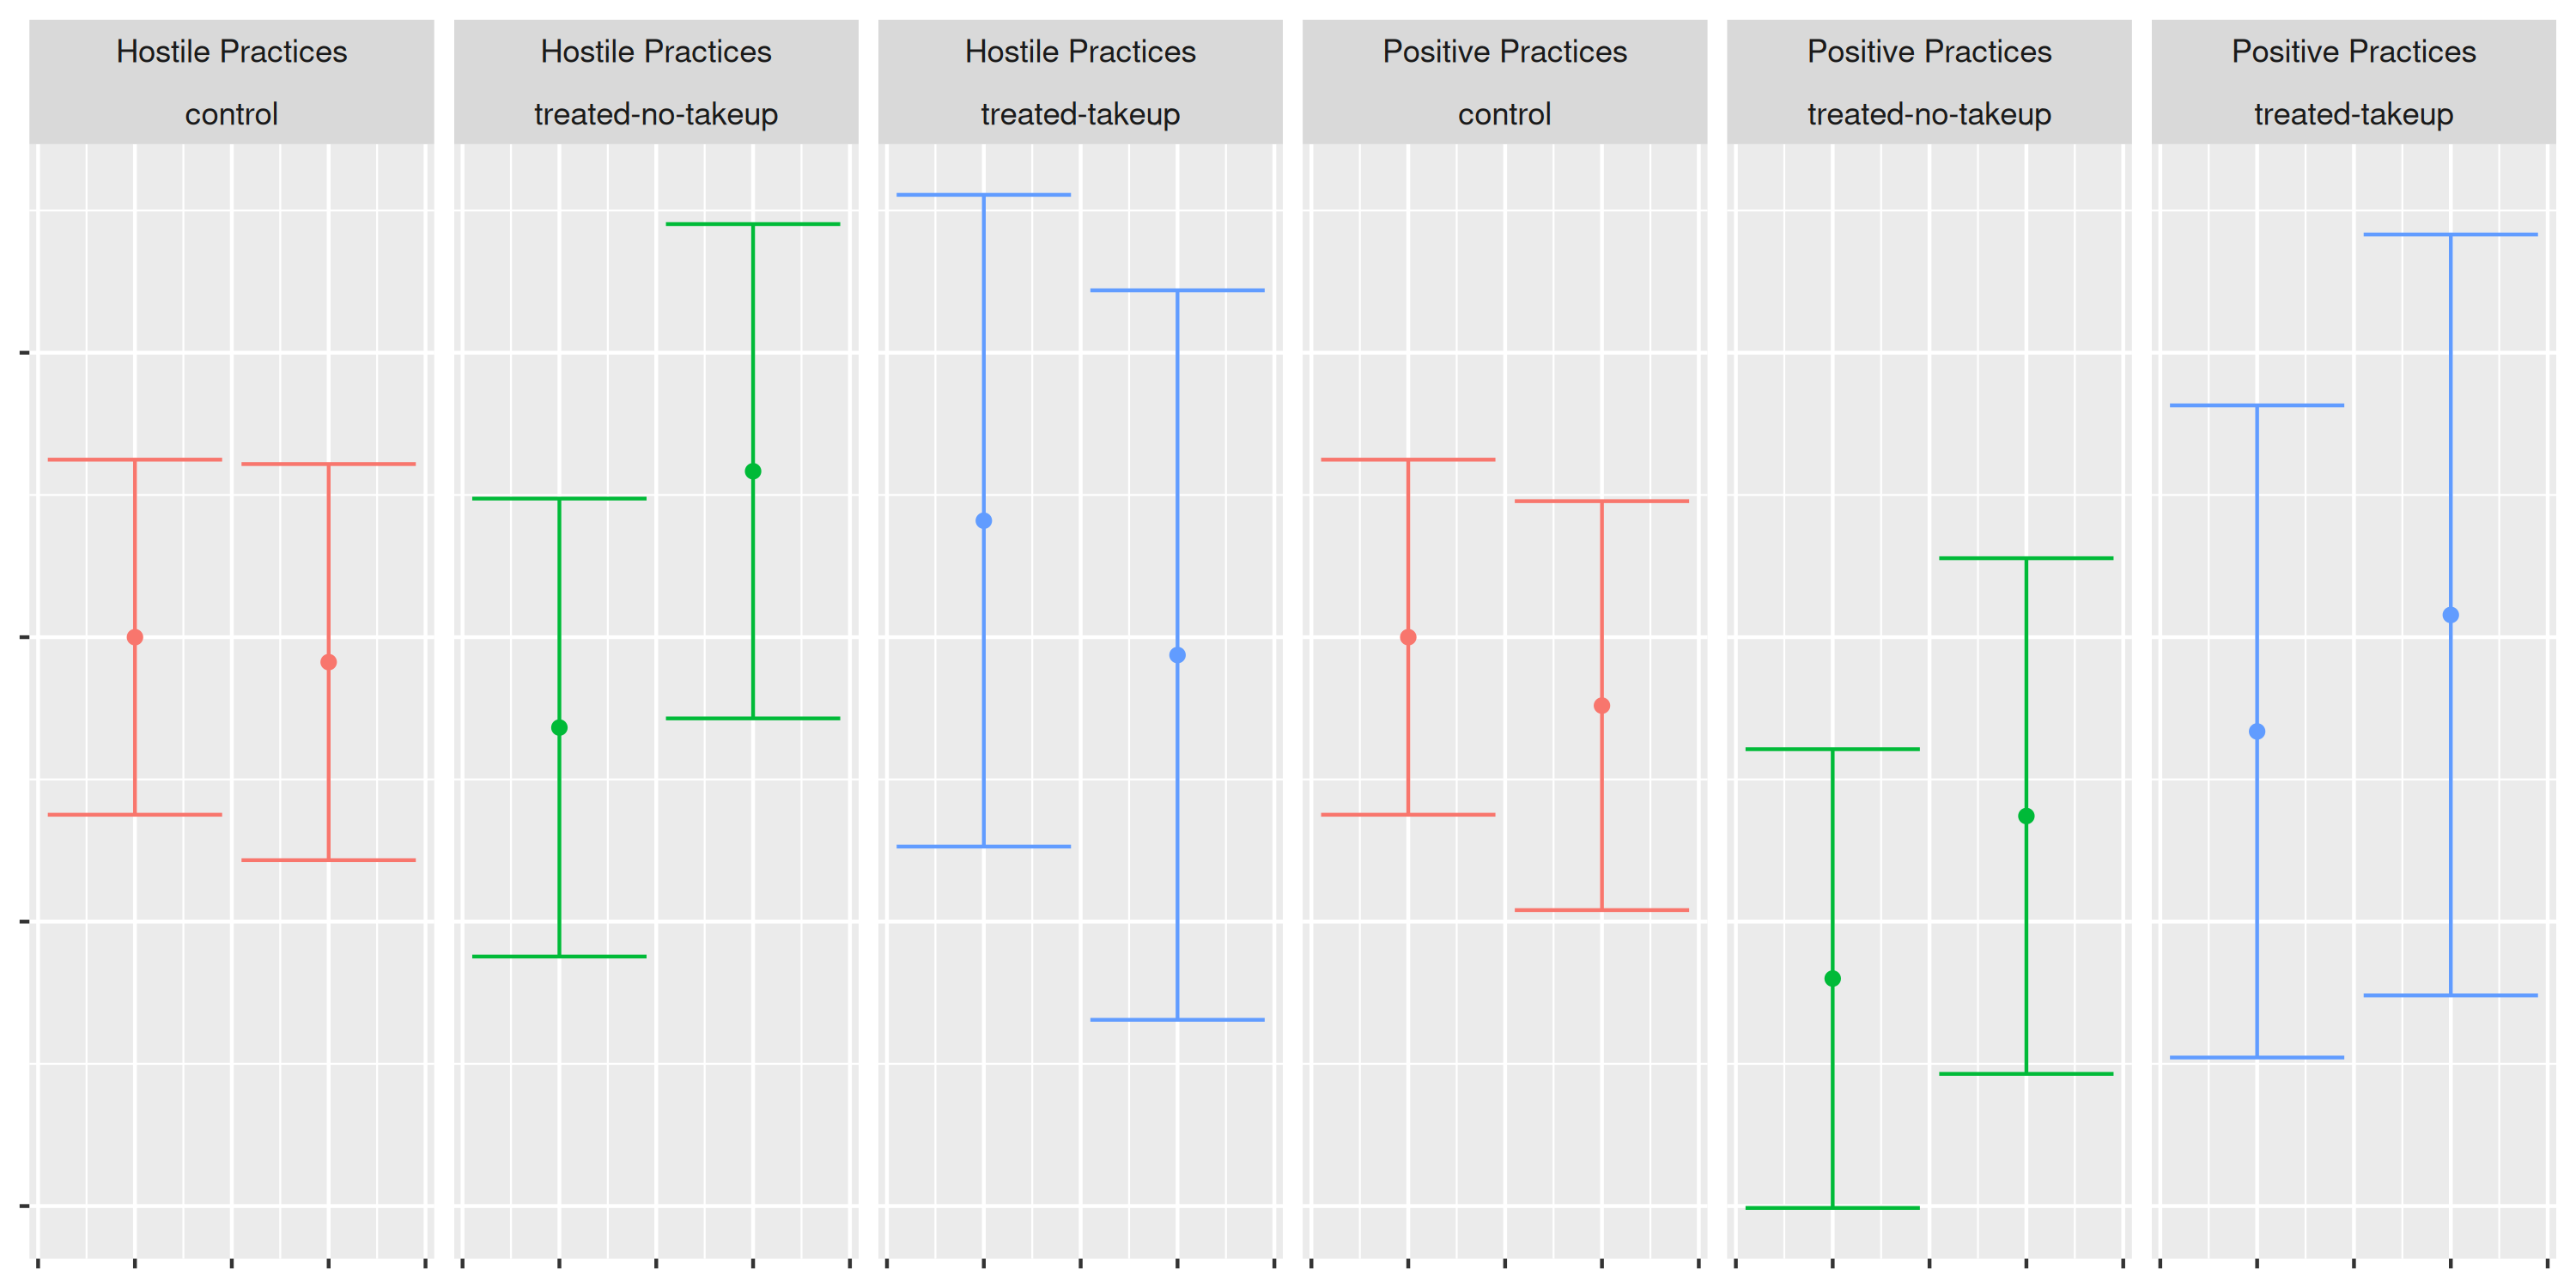
\includegraphics[width=0.9\textwidth]{plots/pre_post/Pooled: Positive Practices.png}

\end{figure}

\addcontentsline{toc}{subsection}{Policy Implications of the Results}
\subsection*{Policy Implications of the Results}

We do not find any significant effect of the use of Bebbo on any of the outcome constructs of interest.

Three reasons, shown in the descriptive data as well as the raw pre-post data might explain why that is the case:
\begin{enumerate}
\item The presence of ceiling effects, where much of the population scored high in the baseline and could not improve in the endline.
\item Priming effects led to participants improving from the first questionnaire to the second questionnaire, regardless of treatment arm and regardless of compliance.
\item Low app usage. While takeup defined as ``had at least one learning event'' was 28\%, which would be enough to measure impacts, it's reasonable to believe that in order to have an impact on these outcomes, especially behaviors and attitudes, participants would need to use the app continuously. Especially if we consider the advantage of an app over a static website or informational fly, the advantage comes through continued usage (it is available on your home screen, can send you push notifications, etc.). Given that only 3\% used the app more than three days, we would not expect to see much of an impact of this app on the population.
\end{enumerate}

Ceiling effects might be a failure in the creation of the survey instrument. They could also be an example in the bias of the sample population (they are all better-than-average caregivers). But there could be a policy implication as well: it could indicate that most caregivers are quite good already at these outcomes, which is important to consider in the means of addressing the problem. In particular: it could indicate the importance of learning about and focusing effort on subgroups that are worse off. Towards that end, we will perform an analysis to determine the characteristics of the ``worse'' caregivers.

Priming effects are a result of the study design, however, they indicate potential policy implications as well. In particular: if asking people questions (``Do you know which vaccine your child needs to take next'') has such a powerful effect on their knowledge, awareness campaigns might be enough to drive results on these outcomes. Knowledge about vaccines and knowledge about child development both seem like good candidates for such an intervention, given this study.

Finally, low app usage implies that either (i) any app must go through extensive testing and improvement before it will be expected to make an impact measurable on a population level or (ii) apps might not be the most effective method of engaging parents. Like any intervention: the implementation matters and each app can be very different. One app failing to engage does not mean that all apps will fail to engage, however, it does leave the possibility open.



\section{User Characteristics Correlated with App Usage}


Given that so few caregivers used the app, it seems important to ask the question: ``who are the respondents who end up as app users?'' We do so by regressing respondents' app usage activity between baseline and endline against their characteristics at baseline. In particular, we will pick two binary outcomes: those who had at least one learning event, who we will say ``Used the App,'' those who had learning events on at least two days, or ``Used More Than 1 Day,'' and finally, those two used the app more than three days.

The results can be found in table \ref{tbl: App Usage}. The regression is formulated as a simple linear regression for ease of interperability. The most notable predictor is whether or not the participant is themselves the parent of the child. The other notable epredictor is ``Activities Past 24h'' which is aligned with what we see in the raw data (under Results), it does seem that in our sample, those who reported doing fewer activities together with their child are more likely to download and use the app. One possible interpretation could be that there is a set of people who are not likely to spend time with their children but are likely to download and use apps. Unfortunately, we do not see a positive impact of this app on those people spending more time with their children, but potentially on a narrow subgroup there might be a positive impact that we do not detect. This could indicate that for ``screen parents'' that are not currently spending time with their children, an app is an effective way to get in front of them. The open question is whether or not it improves their behavior.

There is some additional evidence that those with young children or more likely to use the app, along with those who have less knowledge of child development, speak the dominant language, and are university educated.


% Table created by stargazer v.5.2.3 by Marek Hlavac, Social Policy Institute. E-mail: marek.hlavac at gmail.com
% Date and time: Mon, Mar 11, 2024 - 10:23:27 PM
% Requires LaTeX packages: dcolumn 
\begin{table}[H] \centering 
  \caption{App Usage} 
  \label{tbl:App Usage} 
\begin{tabular}{@{\extracolsep{5pt}}lD{.}{.}{-2} D{.}{.}{-2} D{.}{.}{-2} } 
\\[-1.8ex]\hline 
\hline \\[-1.8ex] 
 & \multicolumn{3}{c}{\textit{Dependent variable:}} \\ 
\cline{2-4} 
\\[-1.8ex] & \multicolumn{1}{c}{Used the App} & \multicolumn{1}{c}{Used More Than 1 Day} & \multicolumn{1}{c}{Used More Than 3 Days} \\ 
\\[-1.8ex] & \multicolumn{1}{c}{(1)} & \multicolumn{1}{c}{(2)} & \multicolumn{1}{c}{(3)}\\ 
\hline \\[-1.8ex] 
 Is Woman & 0.04$ $(0.04) & 0.01$ $(0.03) & -0.02$ $(0.02) \\ 
  University Educated & 0.04$ $(0.03) & 0.03$ $(0.03) & -0.004$ $(0.01) \\ 
  Speaks Dominant Lang. & 0.07$ $(0.07) & 0.02$ $(0.05) & 0.01$ $(0.03) \\ 
  Is Parent & 0.21^{***}$ $(0.06) & 0.12^{***}$ $(0.05) & 0.04$ $(0.02) \\ 
  Child Age & -0.02$ $(0.03) & -0.04^{*}$ $(0.02) & -0.02^{*}$ $(0.01) \\ 
  Num. Children & 0.01$ $(0.06) & 0.01$ $(0.05) & -0.01$ $(0.02) \\ 
  Parent Age & 0.03$ $(0.04) & 0.02$ $(0.03) & 0.01$ $(0.01) \\ 
  Urban Area & -0.02$ $(0.03) & 0.01$ $(0.02) & 0.01$ $(0.01) \\ 
  Child Dev. Knowledge & 0.05$ $(0.07) & -0.04$ $(0.05) & 0.03$ $(0.03) \\ 
  Parenting Confidence & -0.02$ $(0.03) & -0.02$ $(0.02) & 0.01$ $(0.01) \\ 
  Attitude to Phys. Punishment & 0.02$ $(0.02) & 0.003$ $(0.01) & 0.004$ $(0.01) \\ 
  Activities Past 24h & -0.04^{***}$ $(0.01) & -0.03^{***}$ $(0.01) & -0.02^{***}$ $(0.01) \\ 
  Positive Practices & 0.02$ $(0.02) & -0.01$ $(0.02) & 0.0002$ $(0.01) \\ 
  Hostile Practices & -0.03$ $(0.02) & 0.01$ $(0.02) & 0.01$ $(0.01) \\ 
  Constant & 0.16$ $(0.15) & 0.26^{**}$ $(0.11) & -0.01$ $(0.06) \\ 
 \hline \\[-1.8ex] 
Observations & \multicolumn{1}{c}{825} & \multicolumn{1}{c}{825} & \multicolumn{1}{c}{825} \\ 
R$^{2}$ & \multicolumn{1}{c}{0.04} & \multicolumn{1}{c}{0.04} & \multicolumn{1}{c}{0.03} \\ 
Adjusted R$^{2}$ & \multicolumn{1}{c}{0.02} & \multicolumn{1}{c}{0.02} & \multicolumn{1}{c}{0.01} \\ 
Residual Std. Error (df = 810) & \multicolumn{1}{c}{0.45} & \multicolumn{1}{c}{0.33} & \multicolumn{1}{c}{0.16} \\ 
F Statistic (df = 14; 810) & \multicolumn{1}{c}{2.17$^{***}$} & \multicolumn{1}{c}{2.17$^{***}$} & \multicolumn{1}{c}{1.76$^{**}$} \\ 
\hline 
\hline \\[-1.8ex] 
\textit{Note:}  & \multicolumn{3}{r}{$^{*}$p$<$0.1; $^{**}$p$<$0.05; $^{***}$p$<$0.01} \\ 
\end{tabular} 
\end{table} 


\section{Conclusions and Reccomendations}

By construction, mobile apps are meant to be used more than once. The promise of a mobile app is that users will continually engage with it. On average, Europeans spent more than two hours each day on apps (Statista - ``Average daily time spent by users in Europe on mobile apps from October 2020 to March 2021'').

In order for the promotion of an app to be effective as a population-level intervention for parenting, it needs to be engaging enough that a large proportion of the target population will use it and continue to use it. By construction, this implies using it more than one day. Unfortunately, in our study population, 76\% of users who complied with the suggestion to download Bebbo abandoned it after the first day and never returned before the endline survey. This is inline with app usage data outside of our study, which shows that over 80\% of users abandon it after one day. Tracking app retention and engagement rates is important and can be done long before an app gets promoted to a broad population. It is not clear, a priori, what kind of app will engage caregivers, but that is a problem that should be solved before investing in promotion and scale, not after.

We were not able to predict app usage accurately from baseline survey characteristics, although it does seem as though parents who are less likely to do activities with their kids are more likely to use a parenting app.

We were not able to detect any statistically significant impact of promoting the app Bebbo on a general population of caregivers with children 0-6 years of age. Given the lack of engagement in the Bebbo app, this is not surprising. That being said, there were other factors that might have contributed to the lack of discovery of an impact that are in-and-of-themselves interesting. In particular:

\begin{enumerate}
\item There seemed to be a priming effect of the baseline survey, especially for questions related to knowledge, such as ``when is your child's next vaccination due.'' That implies that asking the question has an impact on caregivers and an awareness campaign might be a cheap and effective way of improving routine vaccination rates. People can find the information, they just need to be reminded to look.
\item The majority of respondents scored either very good or perfectly on the baseline assessment. If the respondents were representative of the general population, this would imply that most caregivers in these countries are already knowledgeable and following many good practices. As opposed to a ``general parenting'' intervention, it might be best to focus interventions on particular practices which are still lagging (i.e. breastfeeding) or focus on particular groups or communities where all practices are lagging.
\end{enumerate}

Taken together, these results lead us to recommend that:

\begin{enumerate}
\item To understand the impact of the Bebbo app among the approximately 5\% of downloaders who end up as regularly users, we recommend relying on qualitative research with the existing users.
\item In its current state, Bebbo cannot be expected to move the needle on a population and must become more engaging to a broader range of caregivers before it can be expected to have significant population-level impact.
\item Awareness campaigns might have a significant impact on many of the outcomes of interest to this study and should be investigated further as potential policies that may be more effective at making a significant population-level impact.
\end{enumerate}


\printbibliography

\appendix

\numberwithin{table}{section}
\numberwithin{figure}{section}


\section{Baseline Balance}

To test for balance between our randomly assigned treatment and control groups, we run an omnibus test, following Hansen and Bowers (2008), to observe standardized differences at baseline and the associated omnibus p-value. Results are reported separately for each country and found in tables \ref{tbl:Baseline Balance Serbia} and \ref{tbl:Baseline Balance Bulgaria}. Following \cite{Altman2014}, we do not change our analysis plan based on these results, but it is worth noting that the Bulgaria data does seem to suffer from slight unusual differences between treatment and control condition and the p-value of the omnibus test is significantly low. All the analysis is also reported for only those respondents in Serbia as well, which serves as a robustness check against any concerns that Bulgarians were randomizes into unlucky groups for our analysis.


% 
% Table created by stargazer v.5.2.3 by Marek Hlavac, Social Policy Institute. E-mail: marek.hlavac at gmail.com
% Date and time: Sun, Jan 21, 2024 - 06:42:02 PM
\begin{table}[!htbp] \centering 
  \caption{Baseline Balance Pooled} 
  \label{tbl:Baseline Balance Pooled} 
\begin{tabular}{@{\extracolsep{5pt}} ccccc} 
\\[-1.8ex]\hline 
\hline \\[-1.8ex] 
 & control\_mean & treatment\_mean & standardized\_diff & z\_score \\ 
\hline \\[-1.8ex] 
health\_knw & $0.73$ & $0.71$ & $$-$0.06$ & $$-$1.20$ \\ 
dev\_knw\_recog & $0.86$ & $0.85$ & $$-$0.04$ & $$-$1.29$ \\ 
confidence & $3.33$ & $3.34$ & $0.01$ & $0.37$ \\ 
attitude & $3.14$ & $3.11$ & $$-$0.04$ & $$-$1.23$ \\ 
was\_breastfed & $0.35$ & $0.39$ & $0.08$ & $1.79$ \\ 
practices\_24 & $4.97$ & $4.87$ & $$-$0.07$ & $$-$2.46$ \\ 
practices\_agree & $3.20$ & $3.19$ & $$-$0.01$ & $$-$0.39$ \\ 
practices\_hostility & $3.03$ & $3.04$ & $0.004$ & $0.12$ \\ 
(health\_knw) & $0.42$ & $0.43$ & $0.02$ & $0.67$ \\ 
(was\_breastfed) & $0.42$ & $0.43$ & $0.02$ & $0.61$ \\ 
\hline \\[-1.8ex] 
\multicolumn{5}{l}{Overall P-Value: 0.134132865981628} \\ 
\end{tabular} 
\end{table} 


% Table created by stargazer v.5.2.3 by Marek Hlavac, Social Policy Institute. E-mail: marek.hlavac at gmail.com
% Date and time: Mon, Mar 11, 2024 - 09:43:35 PM
\begin{table}[!htbp] \centering 
  \caption{Baseline Balance Serbia} 
  \label{tbl:Baseline Balance Serbia} 
\begin{tabular}{@{\extracolsep{5pt}} ccccc} 
\\[-1.8ex]\hline 
\hline \\[-1.8ex] 
 & control\_mean & treatment\_mean & standardized\_diff & z\_score \\ 
\hline \\[-1.8ex] 
health\_knw & $0.78$ & $0.75$ & $$-$0.07$ & $$-$1.16$ \\ 
dev\_knw\_recog & $0.87$ & $0.88$ & $0.02$ & $0.62$ \\ 
confidence & $3.38$ & $3.39$ & $0.02$ & $0.57$ \\ 
attitude & $3.08$ & $3.08$ & $$-$0.01$ & $$-$0.17$ \\ 
was\_breastfed & $0.39$ & $0.42$ & $0.07$ & $1.19$ \\ 
practices\_24 & $5.09$ & $4.99$ & $$-$0.09$ & $$-$2.39$ \\ 
practices\_agree & $2.95$ & $2.94$ & $$-$0.02$ & $$-$0.42$ \\ 
practices\_hostility & $3.07$ & $3.05$ & $$-$0.03$ & $$-$0.75$ \\ 
(health\_knw) & $0.40$ & $0.41$ & $0.02$ & $0.63$ \\ 
\hline \\[-1.8ex] 
\multicolumn{5}{l}{Overall P-Value: 0.307} \\ 
\end{tabular} 
\end{table} 


% Table created by stargazer v.5.2.3 by Marek Hlavac, Social Policy Institute. E-mail: marek.hlavac at gmail.com
% Date and time: Tue, Mar 12, 2024 - 11:42:36 PM
\begin{table}[!htbp] \centering 
  \caption{Baseline Balance Bulgaria} 
  \label{tbl:Baseline Balance Bulgaria} 
\begin{tabular}{@{\extracolsep{5pt}} ccccc} 
\\[-1.8ex]\hline 
\hline \\[-1.8ex] 
 & control\_mean & treatment\_mean & standardized\_diff & z\_score \\ 
\hline \\[-1.8ex] 
health\_knw & $0.67$ & $0.65$ & $$-$0.04$ & $$-$0.56$ \\ 
dev\_knw\_recog & $0.85$ & $0.81$ & $$-$0.13$ & $$-$2.71$ \\ 
confidence & $3.27$ & $3.26$ & $$-$0.01$ & $$-$0.21$ \\ 
attitude & $3.23$ & $3.16$ & $$-$0.08$ & $$-$1.57$ \\ 
was\_breastfed & $0.31$ & $0.35$ & $0.10$ & $1.37$ \\ 
practices\_24 & $4.78$ & $4.71$ & $$-$0.06$ & $$-$1.15$ \\ 
practices\_agree & $3.59$ & $3.59$ & $0.02$ & $0.37$ \\ 
practices\_hostility & $2.97$ & $3.00$ & $0.05$ & $1.06$ \\ 
(health\_knw) & $0.45$ & $0.46$ & $0.02$ & $0.40$ \\ 
(was\_breastfed) & $0.45$ & $0.46$ & $0.01$ & $0.30$ \\ 
\hline \\[-1.8ex] 
\multicolumn{5}{l}{Overall P-Value: 0.034} \\ 
\end{tabular} 
\end{table} 


\section{Additional Plots}

\begin{figure}[H]
\begin{minipage}{.5\textwidth}
    \centering
    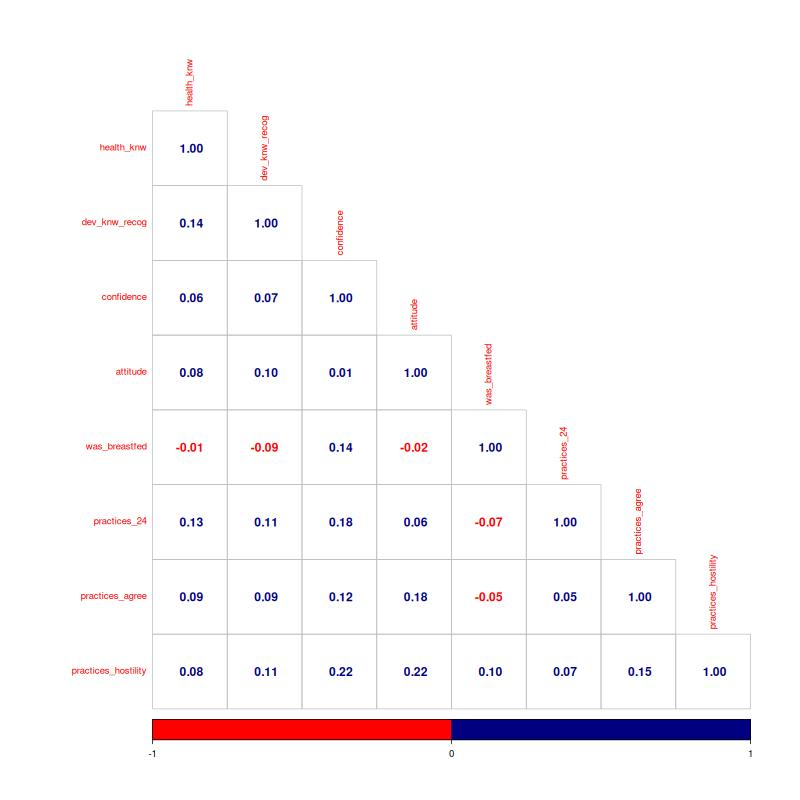
\includegraphics[scale=0.33]{descriptives/plots/correlations_constructs_Serbia_Baseline.jpg}
    \caption{Construct Correlations - Serbia}
    \label{fig:serbia correlations}
\end{minipage}%
\begin{minipage}{.5\textwidth}
    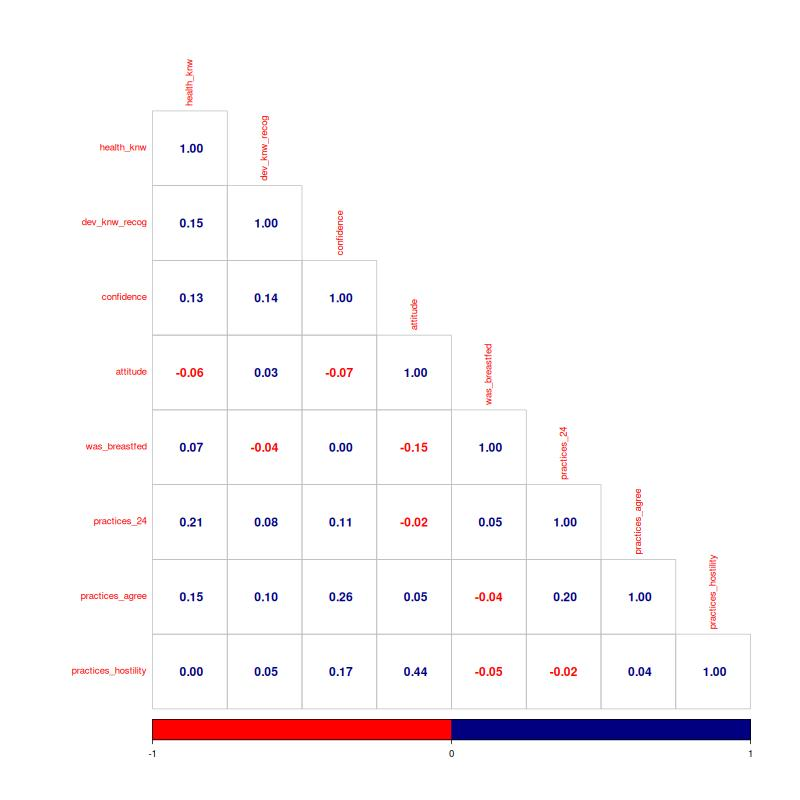
\includegraphics[scale=0.33]{descriptives/plots/correlations_constructs_Bulgaria_Baseline.jpg}
    \caption{Construct Correlations - Bulgaria}
    \label{fig:bulgaria correlations}
\end{minipage}%
\end{figure}

\begin{figure}[H]
  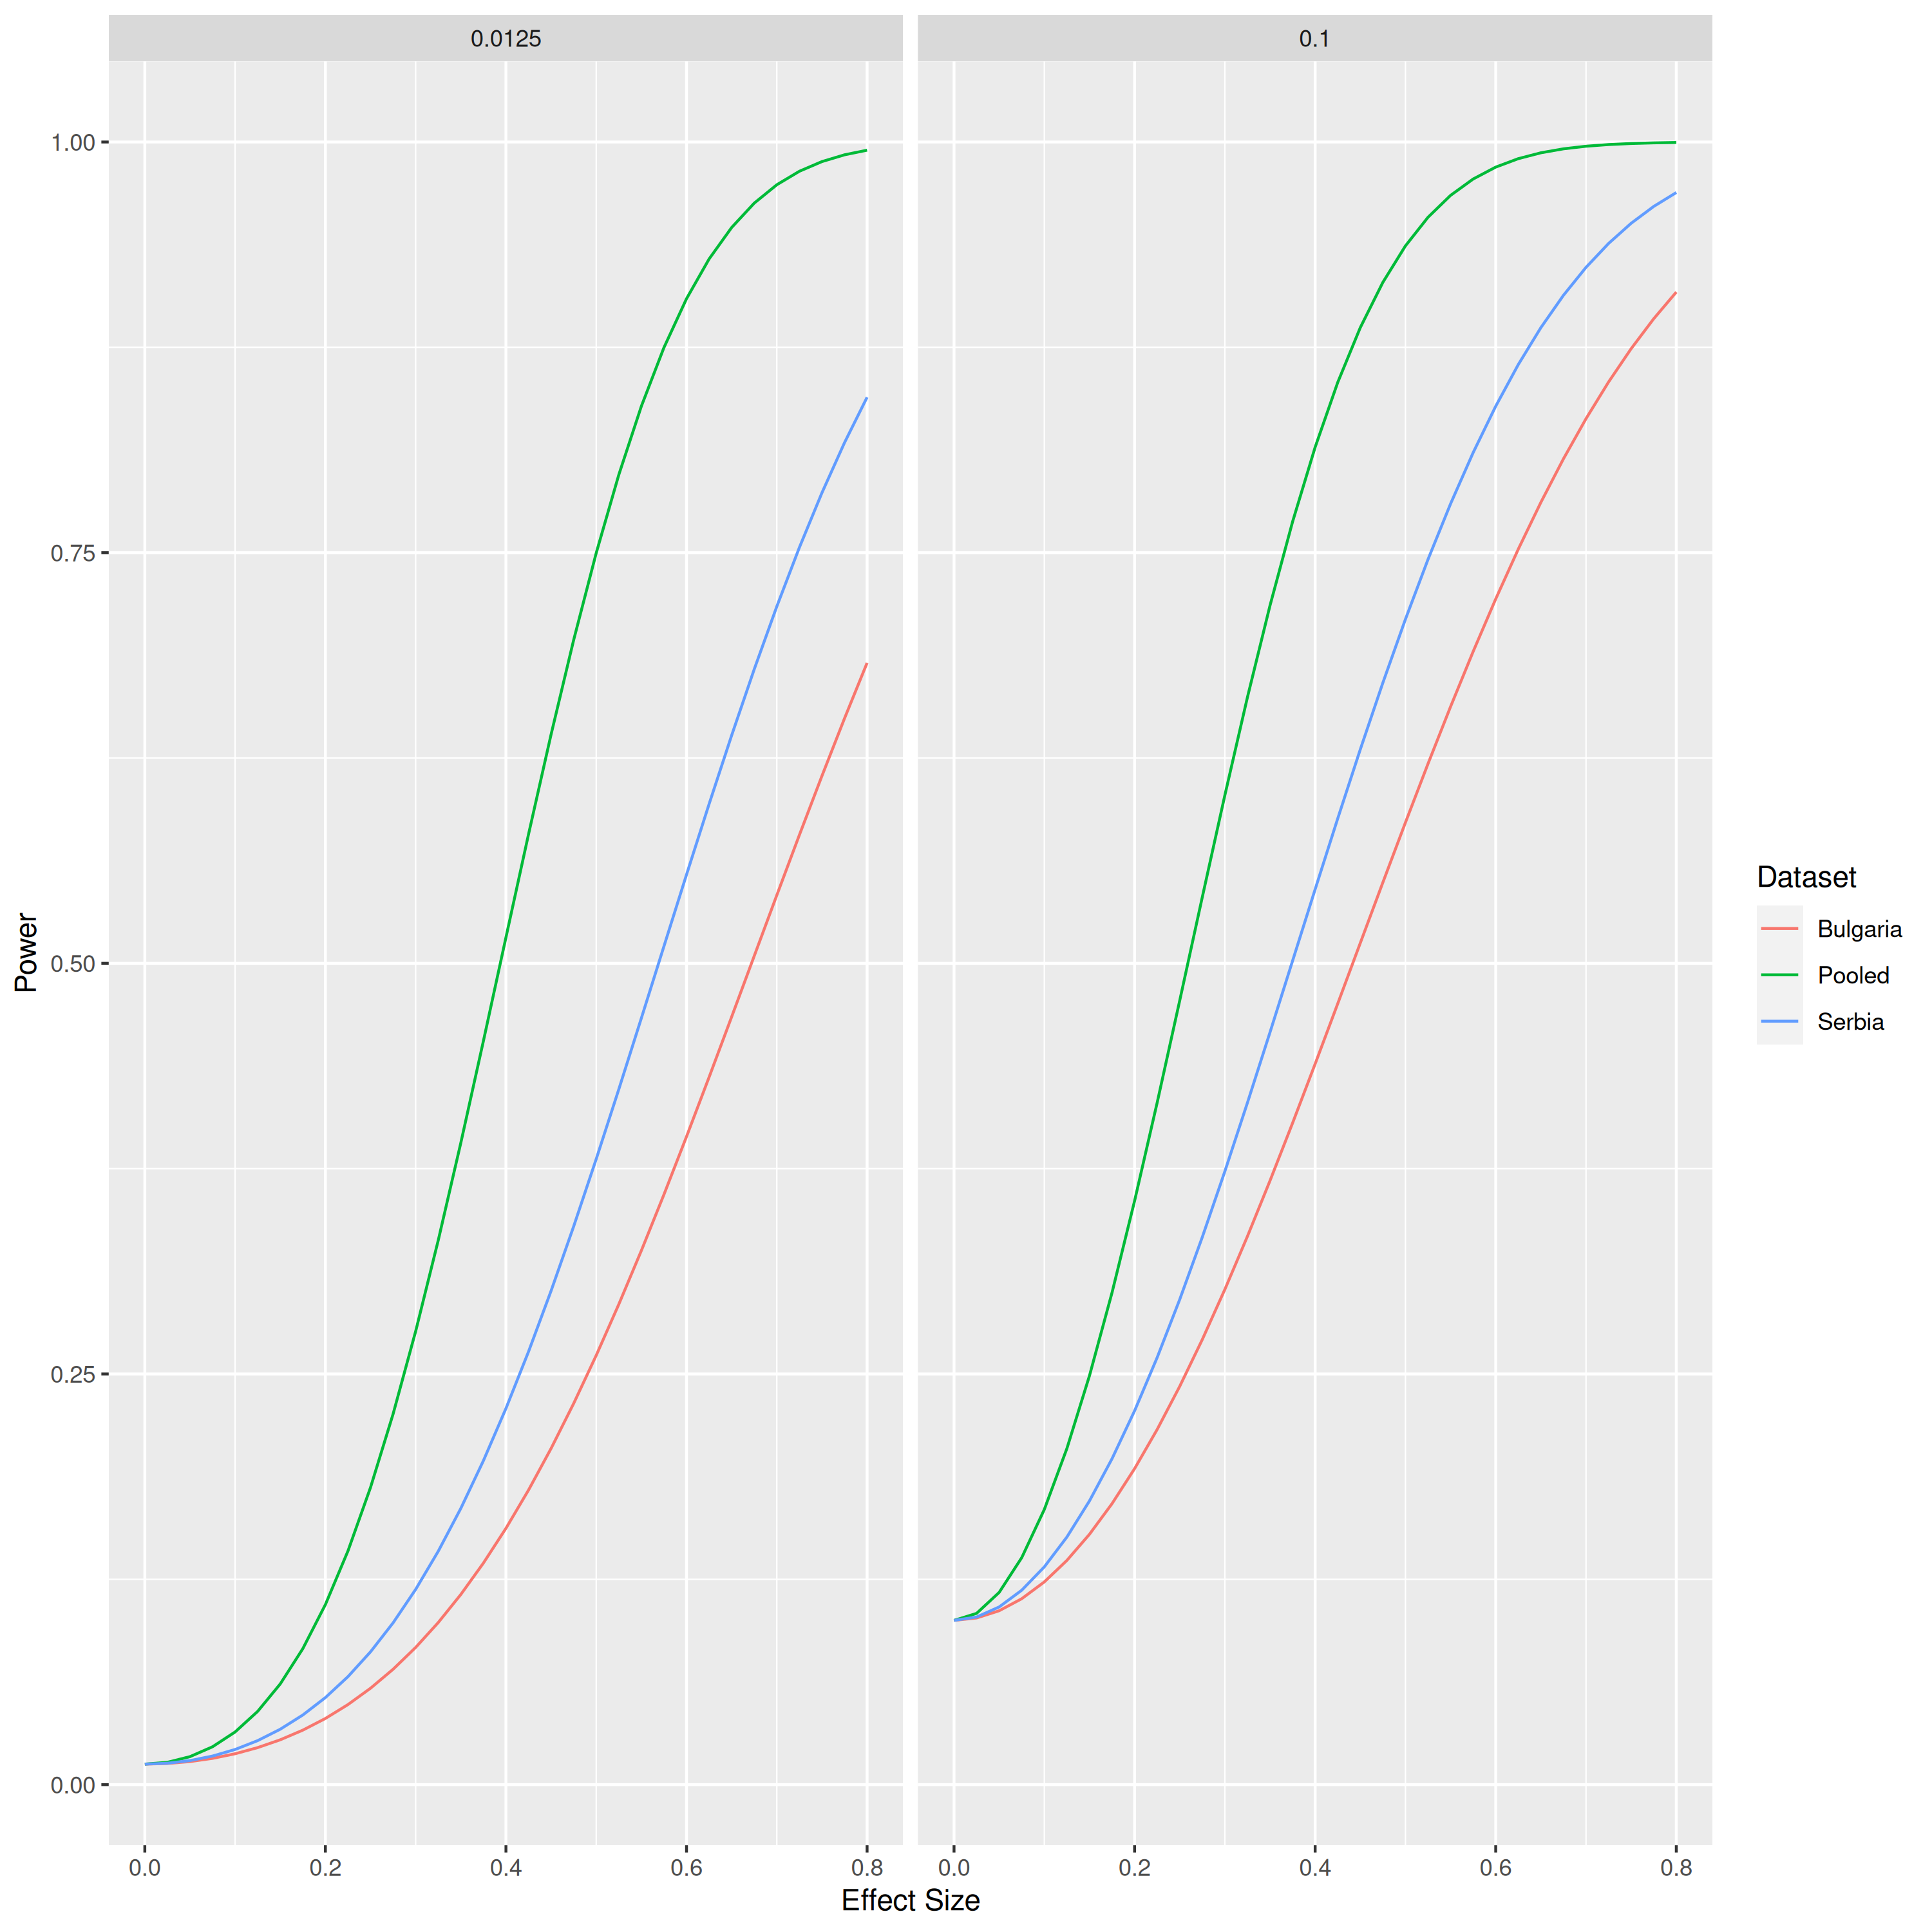
\includegraphics[width=1.0\textwidth]{plots/Power Calculations.png}
  \caption{Power Analysis at 28\% Takeup}
  \label{fig:Power Analysis}
\end{figure}

\clearpage


\begin{figure}[H]
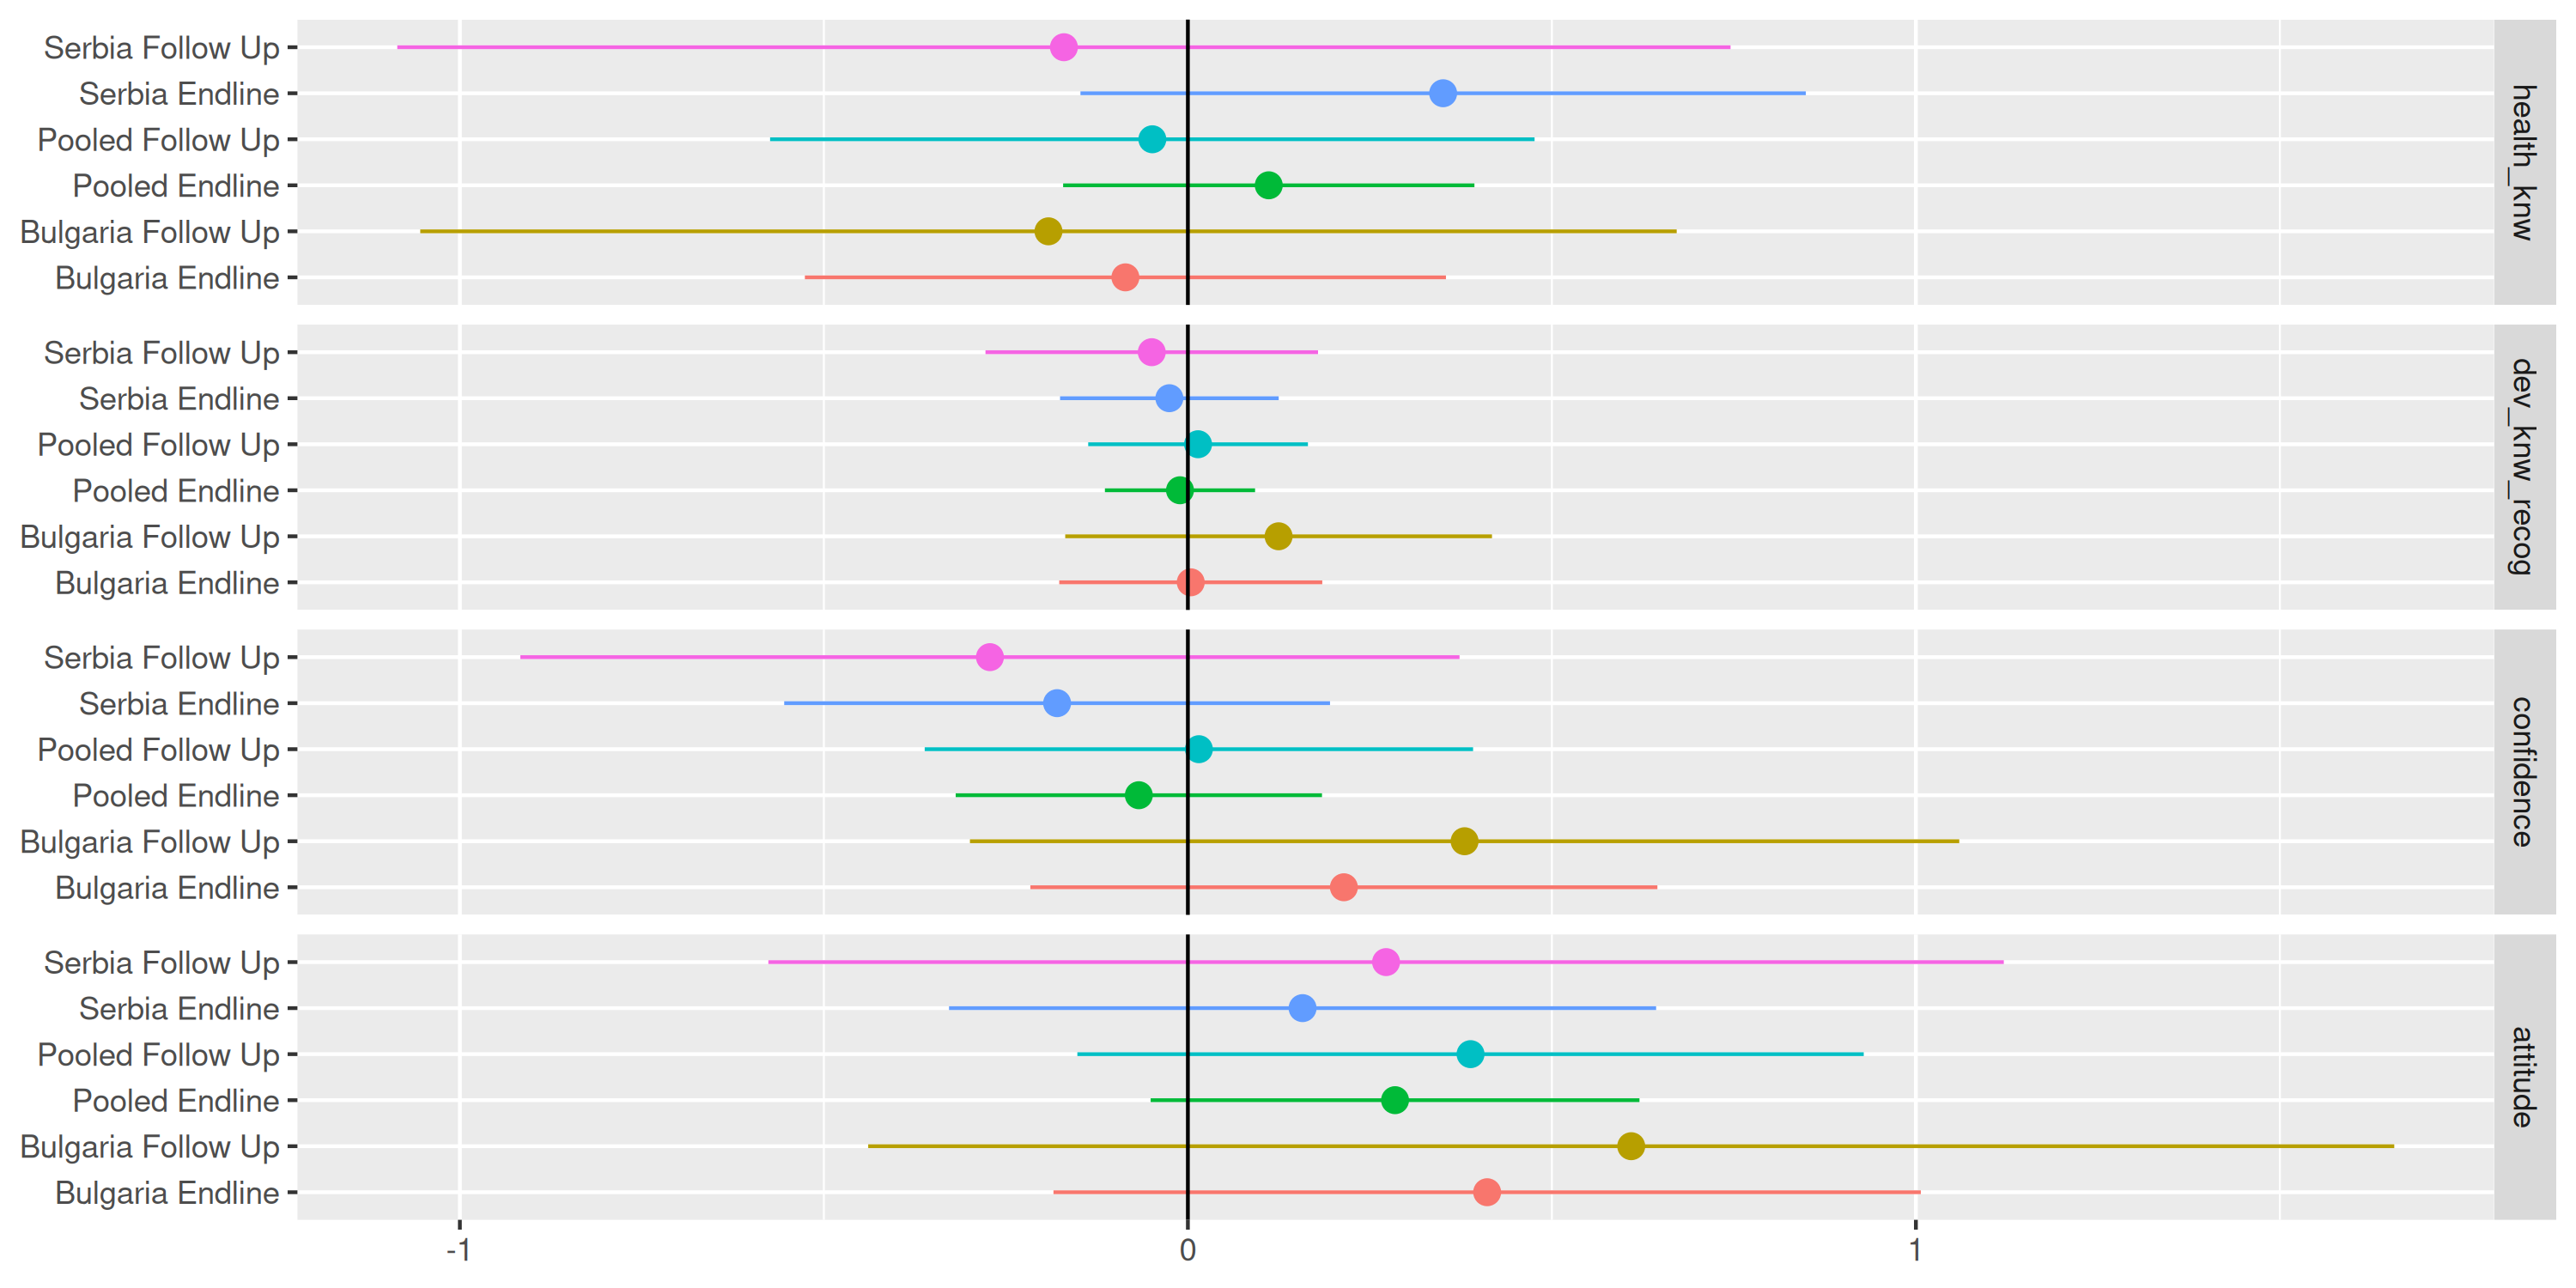
\includegraphics[width=\textwidth]{plots/Adjusted Coefficient Plot Knowledge and Attitudes.png}
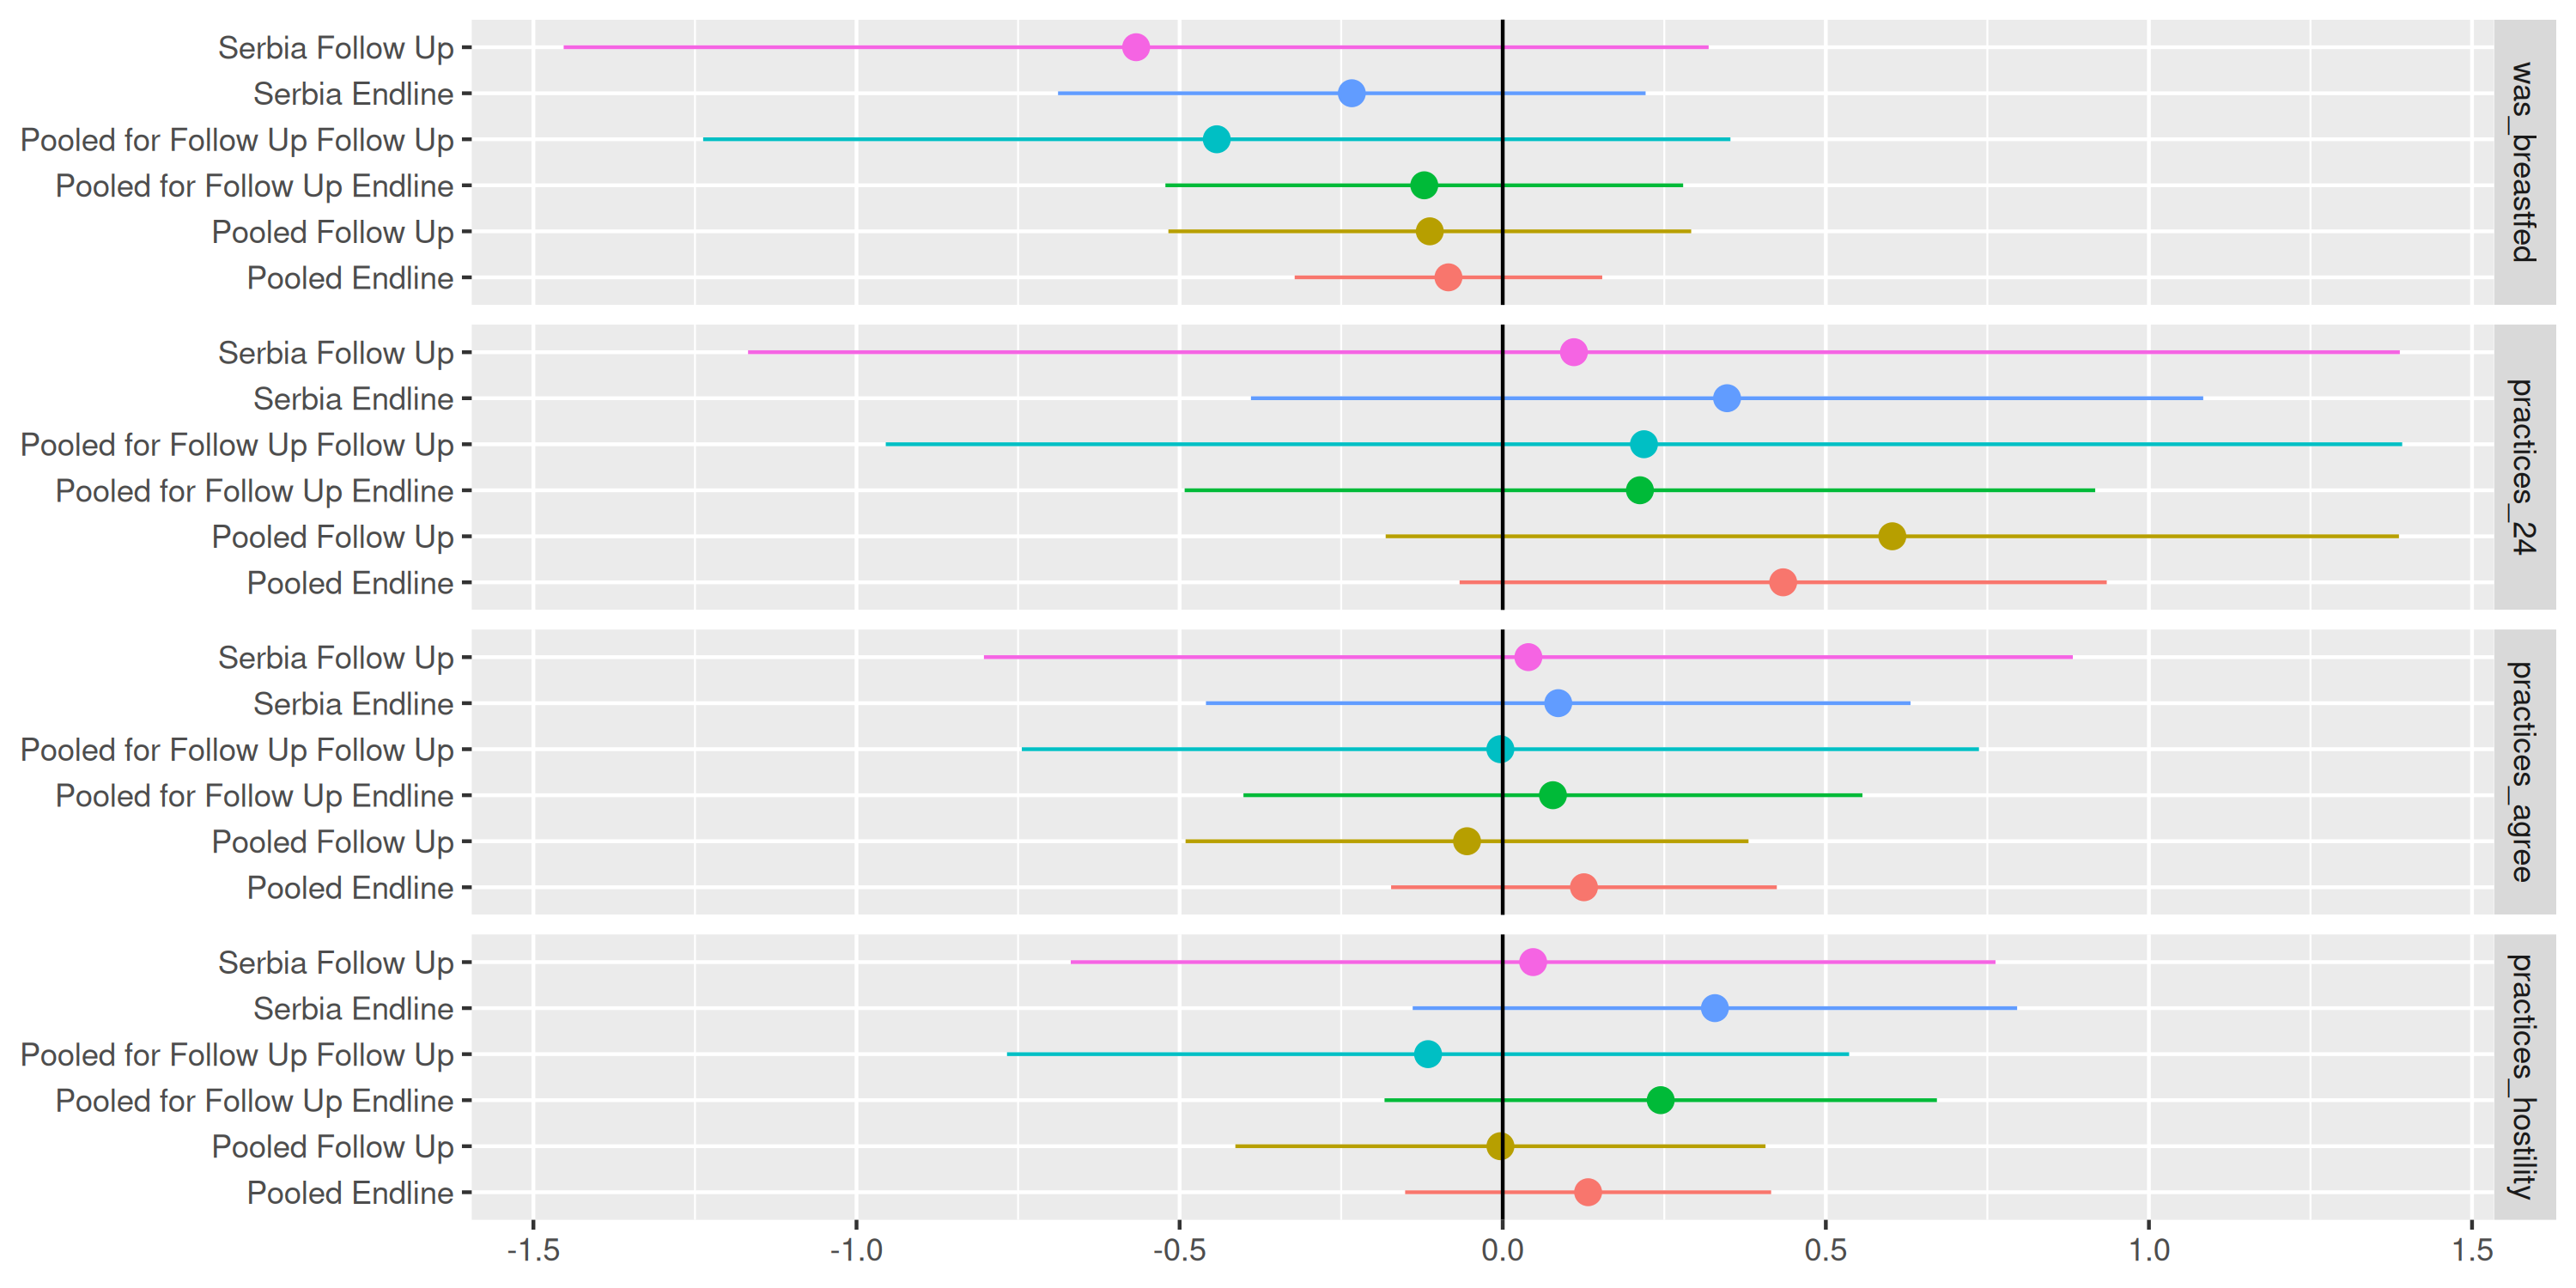
\includegraphics[width=\textwidth]{plots/Adjusted Coefficient Plot Practices.png}
\caption{Adjusted Coefficient Plots of 2SLS in Pooled Dataset}
\end{figure}

\section{Additional Tables}


% Table created by stargazer v.5.2.3 by Marek Hlavac, Social Policy Institute. E-mail: marek.hlavac at gmail.com
% Date and time: Sat, Feb 10, 2024 - 03:00:40 PM
% Requires LaTeX packages: dcolumn 
\begin{table}[!htbp] \centering 
  \caption{Outcome Construct Descriptives Serbia Baseline} 
  \label{tbl:Outcome Construct Descriptives Serbia Baseline} 
\begin{tabular}{@{\extracolsep{5pt}} D{.}{.}{-2} D{.}{.}{-2} D{.}{.}{-2} D{.}{.}{-2} D{.}{.}{-2} D{.}{.}{-2} D{.}{.}{-2} D{.}{.}{-2} } 
\\[-1.8ex]\hline 
\hline \\[-1.8ex] 
\multicolumn{1}{c}{name} & \multicolumn{1}{c}{mean} & \multicolumn{1}{c}{median} & \multicolumn{1}{c}{min} & \multicolumn{1}{c}{max} & \multicolumn{1}{c}{sd} & \multicolumn{1}{c}{prop\_max} & \multicolumn{1}{c}{prop\_na} \\ 
\hline \\[-1.8ex] 
\multicolumn{1}{c}{Activities Past 24h} & \multicolumn{1}{c}{5.06} & \multicolumn{1}{c}{5.0} & \multicolumn{1}{c}{0} & \multicolumn{1}{c}{6} & \multicolumn{1}{c}{1.16} & \multicolumn{1}{c}{0.46} & \multicolumn{1}{c}{0.00} \\ 
\multicolumn{1}{c}{Parenting Confidence} & \multicolumn{1}{c}{3.41} & \multicolumn{1}{c}{3.5} & \multicolumn{1}{c}{1} & \multicolumn{1}{c}{4} & \multicolumn{1}{c}{0.65} & \multicolumn{1}{c}{0.43} & \multicolumn{1}{c}{0.00} \\ 
\multicolumn{1}{c}{Hostile Practices} & \multicolumn{1}{c}{3.06} & \multicolumn{1}{c}{3.0} & \multicolumn{1}{c}{1} & \multicolumn{1}{c}{4} & \multicolumn{1}{c}{0.67} & \multicolumn{1}{c}{0.18} & \multicolumn{1}{c}{0.00} \\ 
\multicolumn{1}{c}{Attitude to Phys. Punishment} & \multicolumn{1}{c}{3.05} & \multicolumn{1}{c}{3.0} & \multicolumn{1}{c}{1} & \multicolumn{1}{c}{4} & \multicolumn{1}{c}{0.82} & \multicolumn{1}{c}{0.31} & \multicolumn{1}{c}{0.00} \\ 
\multicolumn{1}{c}{Positive Practices} & \multicolumn{1}{c}{2.93} & \multicolumn{1}{c}{3.0} & \multicolumn{1}{c}{1} & \multicolumn{1}{c}{4} & \multicolumn{1}{c}{0.81} & \multicolumn{1}{c}{0.24} & \multicolumn{1}{c}{0.00} \\ 
\multicolumn{1}{c}{Child Dev. Knowledge} & \multicolumn{1}{c}{0.87} & \multicolumn{1}{c}{1.0} & \multicolumn{1}{c}{0} & \multicolumn{1}{c}{1} & \multicolumn{1}{c}{0.27} & \multicolumn{1}{c}{0.76} & \multicolumn{1}{c}{0.00} \\ 
\multicolumn{1}{c}{Vaccine Knowledge} & \multicolumn{1}{c}{0.76} & \multicolumn{1}{c}{1.0} & \multicolumn{1}{c}{0} & \multicolumn{1}{c}{1} & \multicolumn{1}{c}{0.43} & \multicolumn{1}{c}{0.76} & \multicolumn{1}{c}{0.61} \\ 
\multicolumn{1}{c}{Breastfed} & \multicolumn{1}{c}{0.41} & \multicolumn{1}{c}{0.0} & \multicolumn{1}{c}{0} & \multicolumn{1}{c}{1} & \multicolumn{1}{c}{0.49} & \multicolumn{1}{c}{0.41} & \multicolumn{1}{c}{0.61} \\ 
\hline \\[-1.8ex] 
\end{tabular} 
\end{table} 


% Table created by stargazer v.5.2.3 by Marek Hlavac, Social Policy Institute. E-mail: marek.hlavac at gmail.com
% Date and time: Mon, Mar 11, 2024 - 09:42:41 PM
% Requires LaTeX packages: dcolumn 
\begin{table}[!htbp] \centering 
  \caption{Outcome Construct Descriptives Bulgaria Baseline} 
  \label{tbl:Outcome Construct Descriptives Bulgaria Baseline} 
\begin{tabular}{@{\extracolsep{5pt}} D{.}{.}{-2} D{.}{.}{-2} D{.}{.}{-2} D{.}{.}{-2} D{.}{.}{-2} D{.}{.}{-2} D{.}{.}{-2} D{.}{.}{-2} } 
\\[-1.8ex]\hline 
\hline \\[-1.8ex] 
\multicolumn{1}{c}{name} & \multicolumn{1}{c}{mean} & \multicolumn{1}{c}{median} & \multicolumn{1}{c}{min} & \multicolumn{1}{c}{max} & \multicolumn{1}{c}{sd} & \multicolumn{1}{c}{prop\_max} & \multicolumn{1}{c}{prop\_na} \\ 
\hline \\[-1.8ex] 
\multicolumn{1}{c}{Activities Past 24h} & \multicolumn{1}{c}{4.72} & \multicolumn{1}{c}{5.00} & \multicolumn{1}{c}{0.0} & \multicolumn{1}{c}{6} & \multicolumn{1}{c}{1.33} & \multicolumn{1}{c}{0.35} & \multicolumn{1}{c}{0.55} \\ 
\multicolumn{1}{c}{Positive Practices} & \multicolumn{1}{c}{3.59} & \multicolumn{1}{c}{3.75} & \multicolumn{1}{c}{1.5} & \multicolumn{1}{c}{4} & \multicolumn{1}{c}{0.40} & \multicolumn{1}{c}{0.32} & \multicolumn{1}{c}{0.55} \\ 
\multicolumn{1}{c}{Parenting Confidence} & \multicolumn{1}{c}{3.27} & \multicolumn{1}{c}{3.50} & \multicolumn{1}{c}{1.0} & \multicolumn{1}{c}{4} & \multicolumn{1}{c}{0.64} & \multicolumn{1}{c}{0.31} & \multicolumn{1}{c}{0.51} \\ 
\multicolumn{1}{c}{Attitude to Phys. Punishment} & \multicolumn{1}{c}{3.20} & \multicolumn{1}{c}{3.00} & \multicolumn{1}{c}{1.0} & \multicolumn{1}{c}{4} & \multicolumn{1}{c}{0.87} & \multicolumn{1}{c}{0.43} & \multicolumn{1}{c}{0.52} \\ 
\multicolumn{1}{c}{Hostile Practices} & \multicolumn{1}{c}{2.99} & \multicolumn{1}{c}{3.00} & \multicolumn{1}{c}{1.0} & \multicolumn{1}{c}{4} & \multicolumn{1}{c}{0.71} & \multicolumn{1}{c}{0.11} & \multicolumn{1}{c}{0.55} \\ 
\multicolumn{1}{c}{Child Dev. Knowledge} & \multicolumn{1}{c}{0.83} & \multicolumn{1}{c}{1.00} & \multicolumn{1}{c}{0.0} & \multicolumn{1}{c}{1} & \multicolumn{1}{c}{0.30} & \multicolumn{1}{c}{0.68} & \multicolumn{1}{c}{0.50} \\ 
\multicolumn{1}{c}{Vaccine Knowledge} & \multicolumn{1}{c}{0.65} & \multicolumn{1}{c}{1.00} & \multicolumn{1}{c}{0.0} & \multicolumn{1}{c}{1} & \multicolumn{1}{c}{0.48} & \multicolumn{1}{c}{0.65} & \multicolumn{1}{c}{0.77} \\ 
\multicolumn{1}{c}{Breastfed} & \multicolumn{1}{c}{0.32} & \multicolumn{1}{c}{0.00} & \multicolumn{1}{c}{0.0} & \multicolumn{1}{c}{1} & \multicolumn{1}{c}{0.47} & \multicolumn{1}{c}{0.32} & \multicolumn{1}{c}{0.79} \\ 
\hline \\[-1.8ex] 
\end{tabular} 
\end{table} 



% Table created by stargazer v.5.2.3 by Marek Hlavac, Social Policy Institute. E-mail: marek.hlavac at gmail.com
% Date and time: Tue, Mar 12, 2024 - 11:42:41 PM
\begin{table}[H] \centering 
  \caption{Attrition: Serbia} 
  \label{tbl:Attrition: Serbia} 
\begin{tabular}{@{\extracolsep{5pt}} cccccc} 
\\[-1.8ex]\hline 
\hline \\[-1.8ex] 
stage & count & attrition & treated\_attrition & control\_attrition & attrition\_dif \\ 
\hline \\[-1.8ex] 
Started Baseline & 5561 &  &  &  &  \\ 
Finished Baseline & 3352 & 0.40 & 0.40 & 0.40 &  0.00 \\ 
Started Endline & 1330 & 0.60 & 0.60 & 0.61 & -0.02 \\ 
Finished Endline & 1270 & 0.05 & 0.06 & 0.03 &  0.03 \\ 
Started Followup &  533 & 0.58 & 0.59 & 0.57 &  0.03 \\ 
Finished Followup &  520 & 0.02 & 0.04 & 0.01 &  0.03 \\ 
\hline \\[-1.8ex] 
\end{tabular} 
\end{table} 


% Table created by stargazer v.5.2.3 by Marek Hlavac, Social Policy Institute. E-mail: marek.hlavac at gmail.com
% Date and time: Mon, Mar 18, 2024 - 11:41:42 PM
\begin{table}[H] \centering 
  \caption{Attrition: Bulgaria} 
  \label{tbl:Attrition: Bulgaria} 
\begin{tabular}{@{\extracolsep{5pt}} cccccc} 
\\[-1.8ex]\hline 
\hline \\[-1.8ex] 
stage & count & attrition & treated\_attrition & control\_attrition & attrition\_dif \\ 
\hline \\[-1.8ex] 
Started Baseline & 4154 &  &  &  &  \\ 
Finished Baseline & 1725 & 0.58 & 0.58 & 0.59 & -0.01 \\ 
Started Endline &  731 & 0.58 & 0.59 & 0.56 &  0.03 \\ 
Finished Endline &  624 & 0.15 & 0.17 & 0.13 &  0.04 \\ 
Started Followup &   36 & 0.94 & 0.95 & 0.94 &  0.02 \\ 
Finished Followup &   35 & 0.03 & 0.07 & 0.00 &  0.07 \\ 
\hline \\[-1.8ex] 
\end{tabular} 
\end{table} 


\section{Additional Regressions}




% Table created by stargazer v.5.2.3 by Marek Hlavac, Social Policy Institute. E-mail: marek.hlavac at gmail.com
% Date and time: Wed, Jan 24, 2024 - 09:15:06 PM
\begin{table}[!htbp] \centering 
  \caption{Pooled: 2SLS - Endline - Knowledge and Awareness} 
  \label{tbl:Pooled: 2SLS - Endline - Knowledge and Awareness} 
\begin{tabular}{@{\extracolsep{5pt}}lcc} 
\\[-1.8ex]\hline 
\hline \\[-1.8ex] 
 & \multicolumn{2}{c}{\textit{Dependent variable:}} \\ 
\cline{2-3} 
\\[-1.8ex] & Vaccine Knowledge & Child Dev. Knowledge \\ 
\\[-1.8ex] & (1) & (2)\\ 
\hline \\[-1.8ex] 
 Used App & 0.10 & $-$0.02 \\ 
  & (0.11) & (0.04) \\ 
  & & \\ 
\hline \\[-1.8ex] 
Adjusted Treatment p-value & 0.695 & 0.714 \\ 
Weak instruments p-value & 1.17e-28 & 2.44e-77 \\ 
Wu-Hausman p-value & 0.849 & 0.355 \\ 
Observations & 696 & 1,931 \\ 
R$^{2}$ & 0.01 & 0.01 \\ 
\hline 
\hline \\[-1.8ex] 
\textit{Note:}  & \multicolumn{2}{r}{$^{*}$p$<$0.1; $^{**}$p$<$0.05; $^{***}$p$<$0.01} \\ 
\end{tabular} 
\end{table} 


% Table created by stargazer v.5.2.3 by Marek Hlavac, Social Policy Institute. E-mail: marek.hlavac at gmail.com
% Date and time: Tue, Mar 12, 2024 - 11:43:23 PM
\begin{table}[!htbp] \centering 
  \caption{Pooled: 2SLS - Endline - Confidence and Attitudes} 
  \label{tbl:Pooled: 2SLS - Endline - Confidence and Attitudes} 
\begin{tabular}{@{\extracolsep{5pt}}lcc} 
\\[-1.8ex]\hline 
\hline \\[-1.8ex] 
 & \multicolumn{2}{c}{\textit{Dependent variable:}} \\ 
\cline{2-3} 
\\[-1.8ex] & Parenting Confidence & Attitude to Phys. Punishment \\ 
\\[-1.8ex] & (1) & (2)\\ 
\hline \\[-1.8ex] 
 Used App & 0.02 & 0.27 \\ 
  & (0.10) & (0.13) \\ 
  & & \\ 
\hline \\[-1.8ex] 
Adjusted Treatment p-value & 0.797 & 0.162 \\ 
Weak instruments p-value & 1.54e-82 & 1.36e-82 \\ 
Wu-Hausman p-value & 0.967 & 0.0465 \\ 
Observations & 1,972 & 1,961 \\ 
R$^{2}$ & 0.01 & $-$0.005 \\ 
\hline 
\hline \\[-1.8ex] 
\textit{Note:}  & \multicolumn{2}{r}{$^{*}$p$<$0.1; $^{**}$p$<$0.05; $^{***}$p$<$0.01} \\ 
\end{tabular} 
\end{table} 


% Table created by stargazer v.5.2.3 by Marek Hlavac, Social Policy Institute. E-mail: marek.hlavac at gmail.com
% Date and time: Tue, Mar 12, 2024 - 11:43:25 PM
\begin{table}[!htbp] \centering 
  \caption{Pooled: 2SLS - Endline - Practices} 
  \label{tbl:Pooled: 2SLS - Endline - Practices} 
\begin{tabular}{@{\extracolsep{5pt}}lcccc} 
\\[-1.8ex]\hline 
\hline \\[-1.8ex] 
 & \multicolumn{4}{c}{\textit{Dependent variable:}} \\ 
\cline{2-5} 
\\[-1.8ex] & Breastfed & Activities Past 24h & Positive Practices & Hostile Practices \\ 
\\[-1.8ex] & (1) & (2) & (3) & (4)\\ 
\hline \\[-1.8ex] 
 Used App & $-$0.05 & 0.41 & 0.10 & 0.09 \\ 
  & (0.09) & (0.18) & (0.11) & (0.10) \\ 
  & & & & \\ 
\hline \\[-1.8ex] 
Adjusted Treatment p-value & 0.714 & 0.162 & 0.619 & 0.619 \\ 
Weak instruments p-value & 3.75e-32 & 1.17e-80 & 6.72e-81 & 4.82e-81 \\ 
Wu-Hausman p-value & 0.963 & 0.0115 & 0.639 & 0.258 \\ 
Observations & 682 & 1,903 & 1,904 & 1,900 \\ 
R$^{2}$ & 0.02 & $-$0.01 & 0.004 & 0.005 \\ 
\hline 
\hline \\[-1.8ex] 
\textit{Note:}  & \multicolumn{4}{r}{$^{*}$p$<$0.1; $^{**}$p$<$0.05; $^{***}$p$<$0.01} \\ 
\end{tabular} 
\end{table} 



% Table created by stargazer v.5.2.3 by Marek Hlavac, Social Policy Institute. E-mail: marek.hlavac at gmail.com
% Date and time: Tue, Mar 12, 2024 - 11:43:07 PM
\begin{table}[!htbp] \centering 
  \caption{Serbia: OLS - Endline - Knowledge and Awareness} 
  \label{tbl:Serbia: OLS - Endline - Knowledge and Awareness} 
\begin{tabular}{@{\extracolsep{5pt}}lcc} 
\\[-1.8ex]\hline 
\hline \\[-1.8ex] 
 & \multicolumn{2}{c}{\textit{Dependent variable:}} \\ 
\cline{2-3} 
\\[-1.8ex] & Vaccine Knowledge & Child Dev. Knowledge \\ 
\\[-1.8ex] & (1) & (2)\\ 
\hline \\[-1.8ex] 
 Treatment & 0.12$^{*}$ & $-$0.01 \\ 
  & (0.05) & (0.02) \\ 
  & & \\ 
\hline \\[-1.8ex] 
Adjusted Treatment p-value & 0.0835 & 0.731 \\ 
Observations & 316 & 984 \\ 
R$^{2}$ & 0.03 & 0.02 \\ 
\hline 
\hline \\[-1.8ex] 
\textit{Note:}  & \multicolumn{2}{r}{$^{*}$p$<$0.1; $^{**}$p$<$0.05; $^{***}$p$<$0.01} \\ 
\end{tabular} 
\end{table} 

\begin{figure}[H]
  \centering
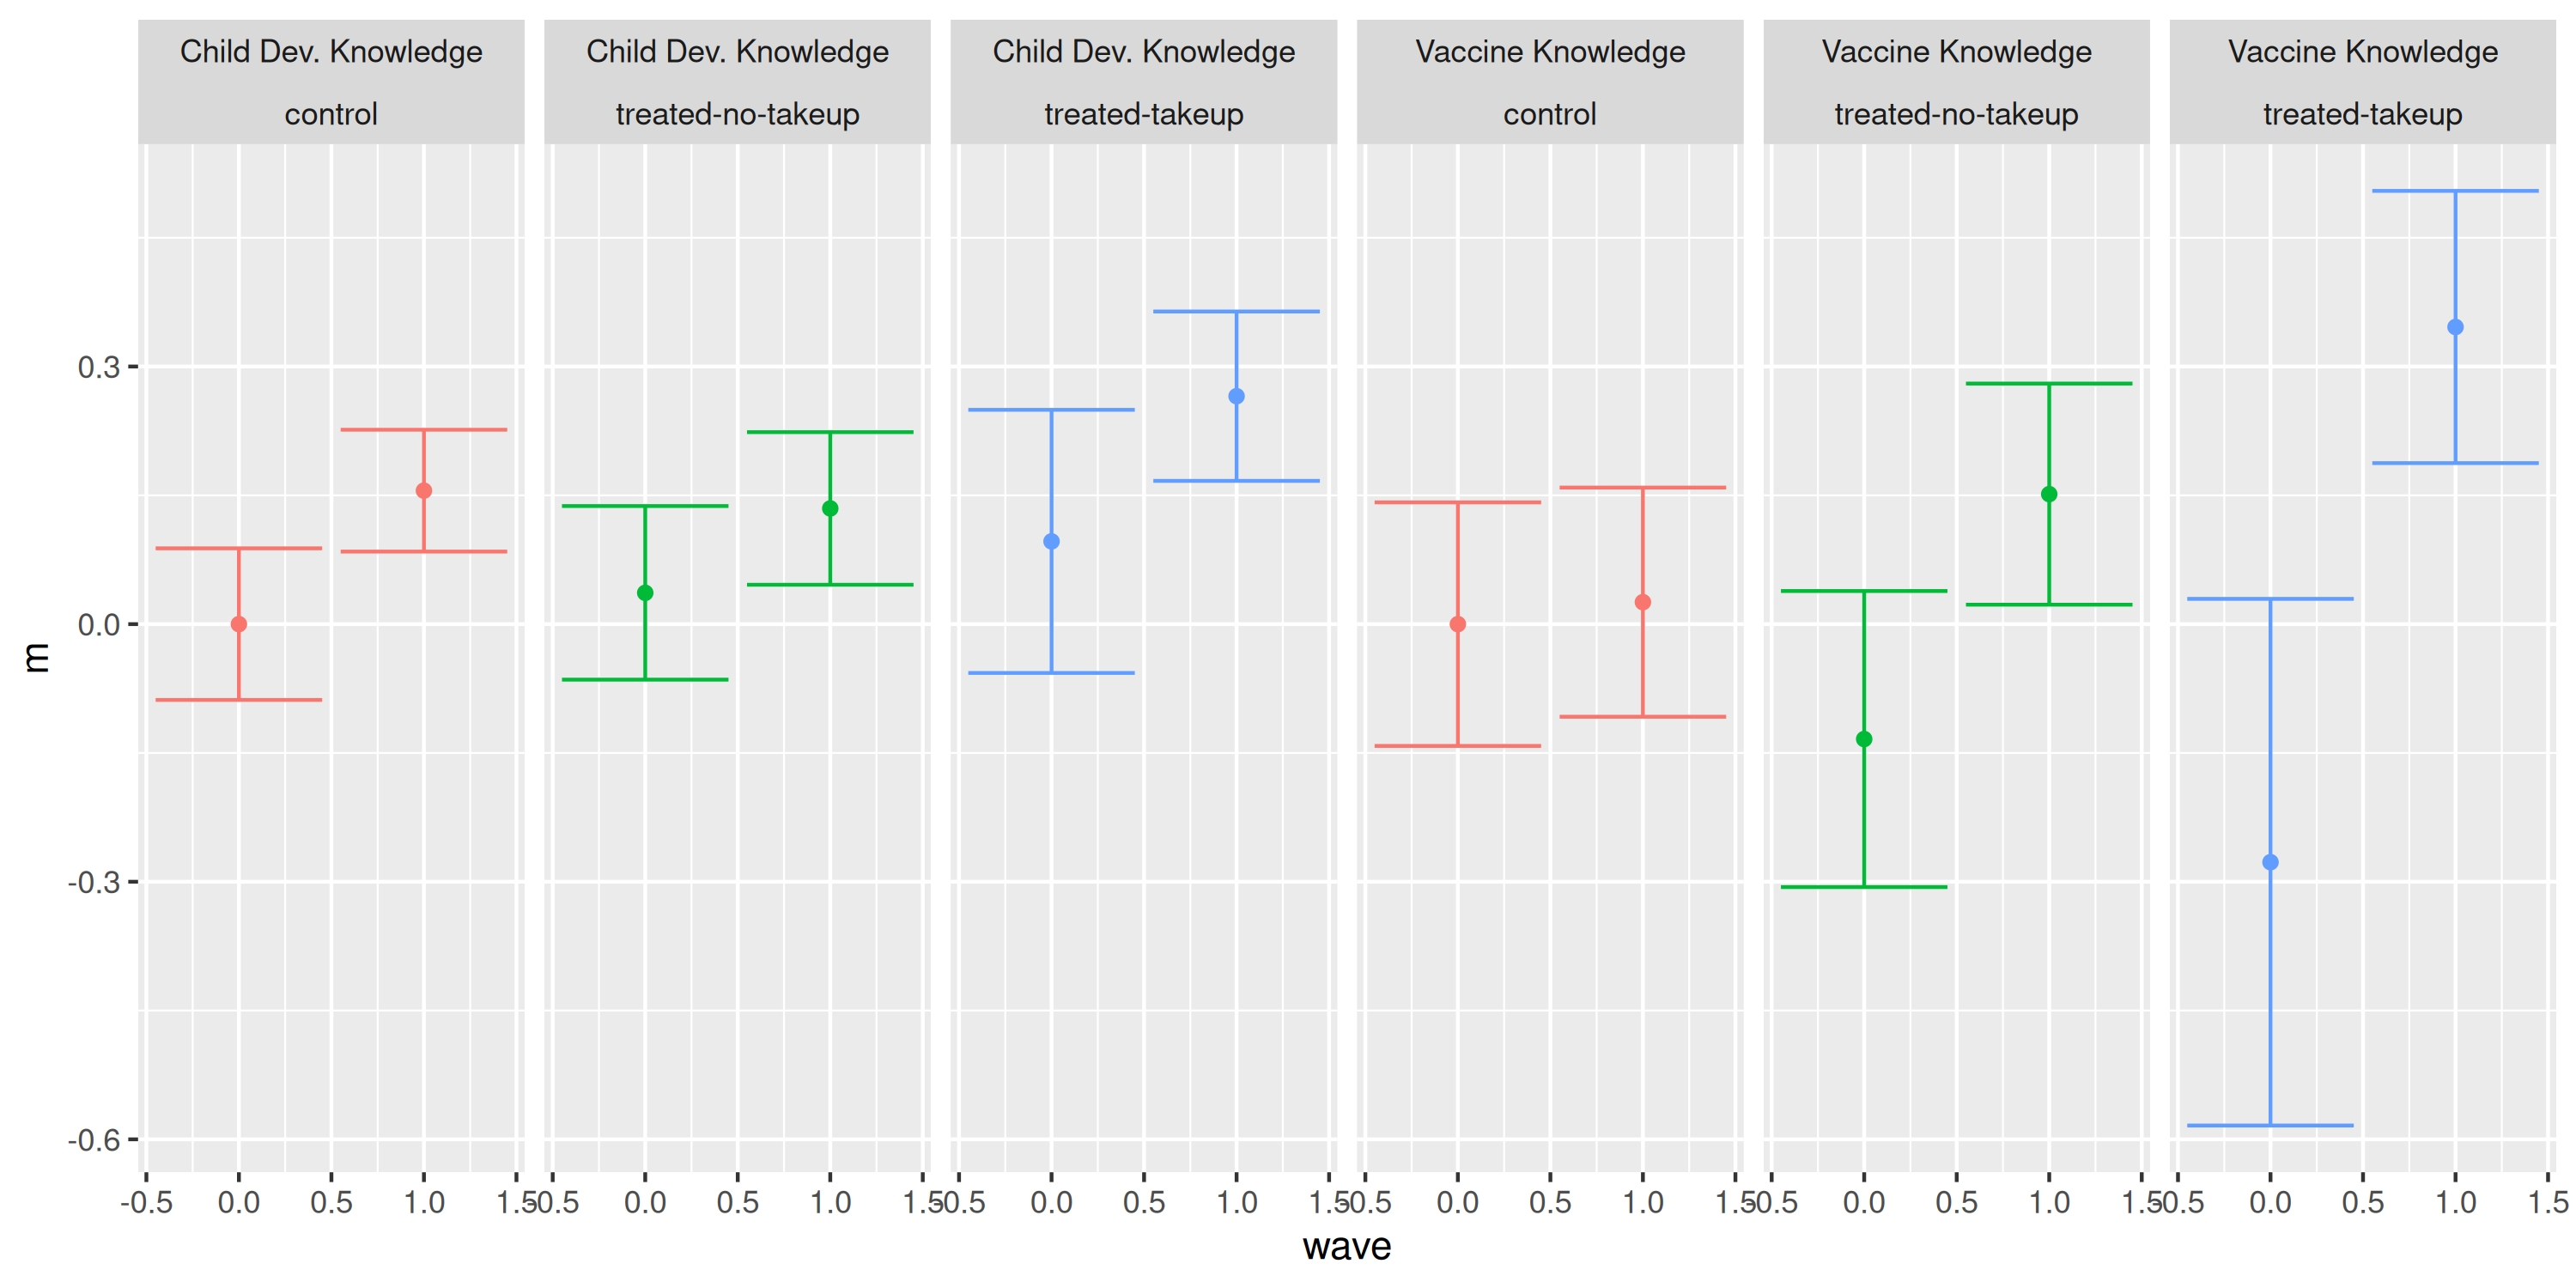
\includegraphics[width=0.9\textwidth]{plots/pre_post/Serbia: Vaccine Knowledge.png}
\end{figure}



% Table created by stargazer v.5.2.3 by Marek Hlavac, Social Policy Institute. E-mail: marek.hlavac at gmail.com
% Date and time: Tue, Mar 12, 2024 - 11:43:08 PM
\begin{table}[!htbp] \centering 
  \caption{Serbia: OLS - Endline - Confidence and Attitudes} 
  \label{tbl:Serbia: OLS - Endline - Confidence and Attitudes} 
\begin{tabular}{@{\extracolsep{5pt}}lcc} 
\\[-1.8ex]\hline 
\hline \\[-1.8ex] 
 & \multicolumn{2}{c}{\textit{Dependent variable:}} \\ 
\cline{2-3} 
\\[-1.8ex] & Parenting Confidence & Attitude to Phys. Punishment \\ 
\\[-1.8ex] & (1) & (2)\\ 
\hline \\[-1.8ex] 
 Treatment & $-$0.01 & 0.03 \\ 
  & (0.04) & (0.05) \\ 
  & & \\ 
\hline \\[-1.8ex] 
Adjusted Treatment p-value & 0.891 & 0.731 \\ 
Observations & 974 & 973 \\ 
R$^{2}$ & 0.02 & 0.01 \\ 
\hline 
\hline \\[-1.8ex] 
\textit{Note:}  & \multicolumn{2}{r}{$^{*}$p$<$0.1; $^{**}$p$<$0.05; $^{***}$p$<$0.01} \\ 
\end{tabular} 
\end{table} 

\begin{figure}[H]
  \centering
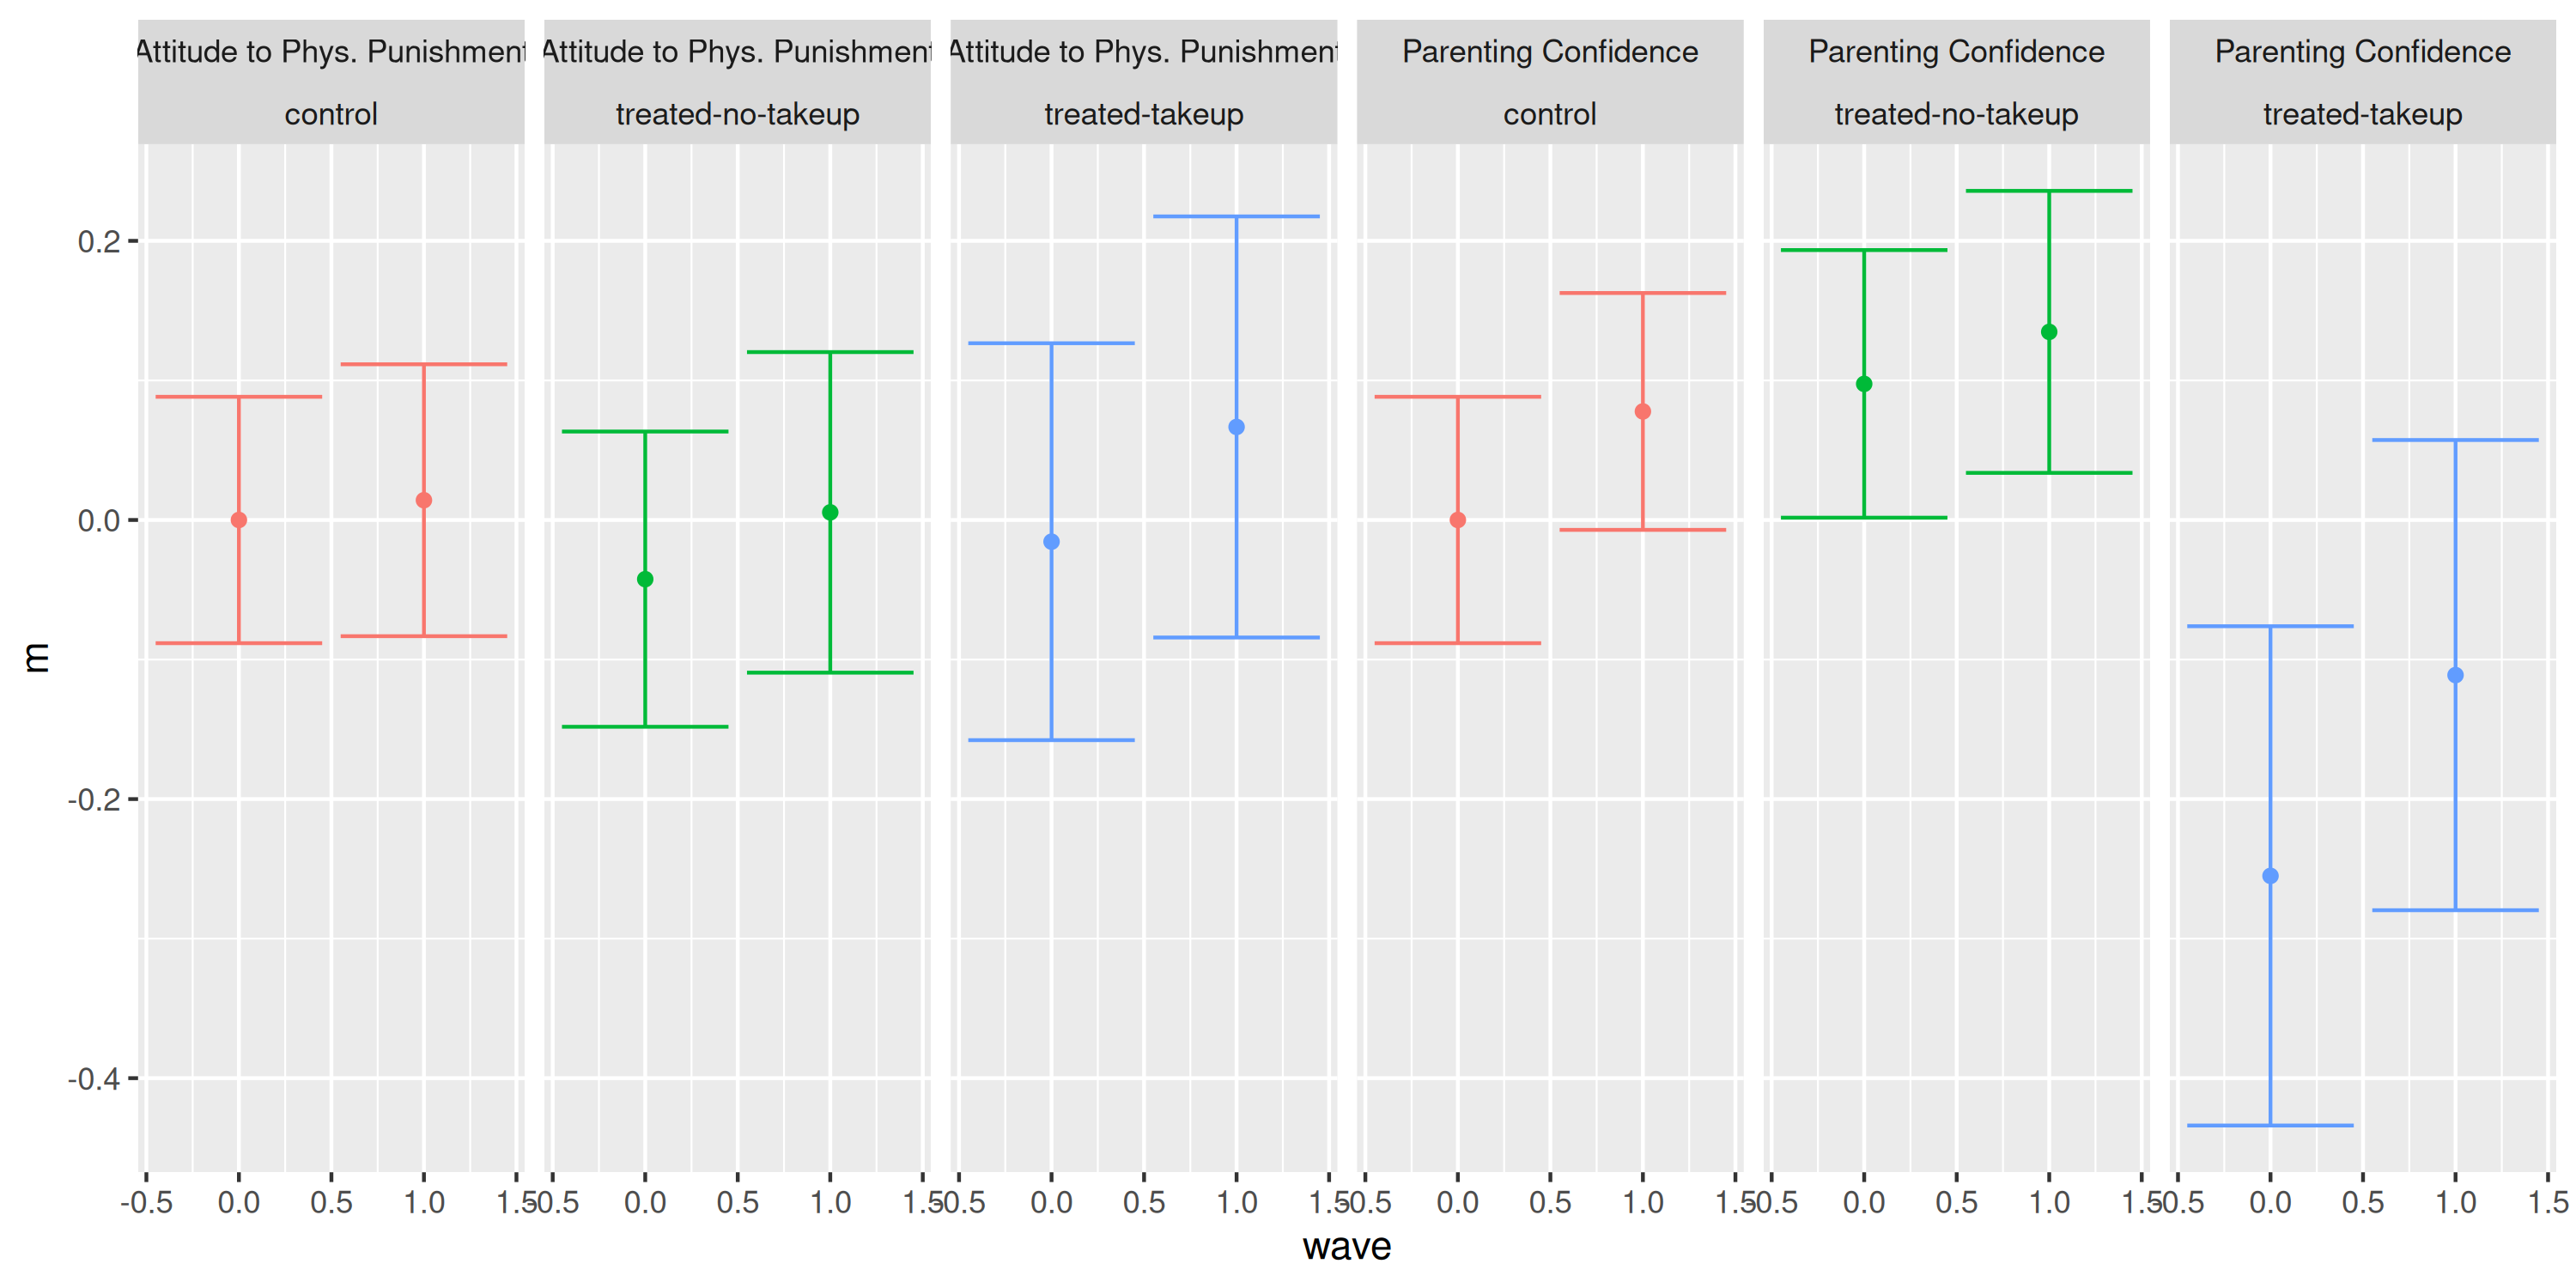
\includegraphics[width=0.9\textwidth]{plots/pre_post/Serbia: Parenting Confidence.png}
\end{figure}



% Table created by stargazer v.5.2.3 by Marek Hlavac, Social Policy Institute. E-mail: marek.hlavac at gmail.com
% Date and time: Mon, Mar 18, 2024 - 11:42:02 PM
\begin{table}[!htbp] \centering 
  \caption{Serbia: OLS - Endline - Practices} 
  \label{tbl:Serbia: OLS - Endline - Practices} 
\begin{tabular}{@{\extracolsep{5pt}}lcccc} 
\\[-1.8ex]\hline 
\hline \\[-1.8ex] 
 & \multicolumn{4}{c}{\textit{Dependent variable:}} \\ 
\cline{2-5} 
\\[-1.8ex] & Breastfed & Activities Past 24h & Positive Practices & Hostile Practices \\ 
\\[-1.8ex] & (1) & (2) & (3) & (4)\\ 
\hline \\[-1.8ex] 
 Treatment & $-$0.03 & 0.10 & 0.01 & 0.05 \\ 
  & (0.04) & (0.07) & (0.05) & (0.05) \\ 
  & & & & \\ 
\hline \\[-1.8ex] 
Adjusted Treatment p-value & 0.731 & 0.704 & 0.891 & 0.704 \\ 
Observations & 304 & 949 & 950 & 948 \\ 
R$^{2}$ & 0.04 & 0.01 & 0.01 & 0.02 \\ 
\hline 
\hline \\[-1.8ex] 
\textit{Note:}  & \multicolumn{4}{r}{$^{*}$p$<$0.1; $^{**}$p$<$0.05; $^{***}$p$<$0.01} \\ 
\end{tabular} 
\end{table} 

\begin{figure}[H]
  \centering
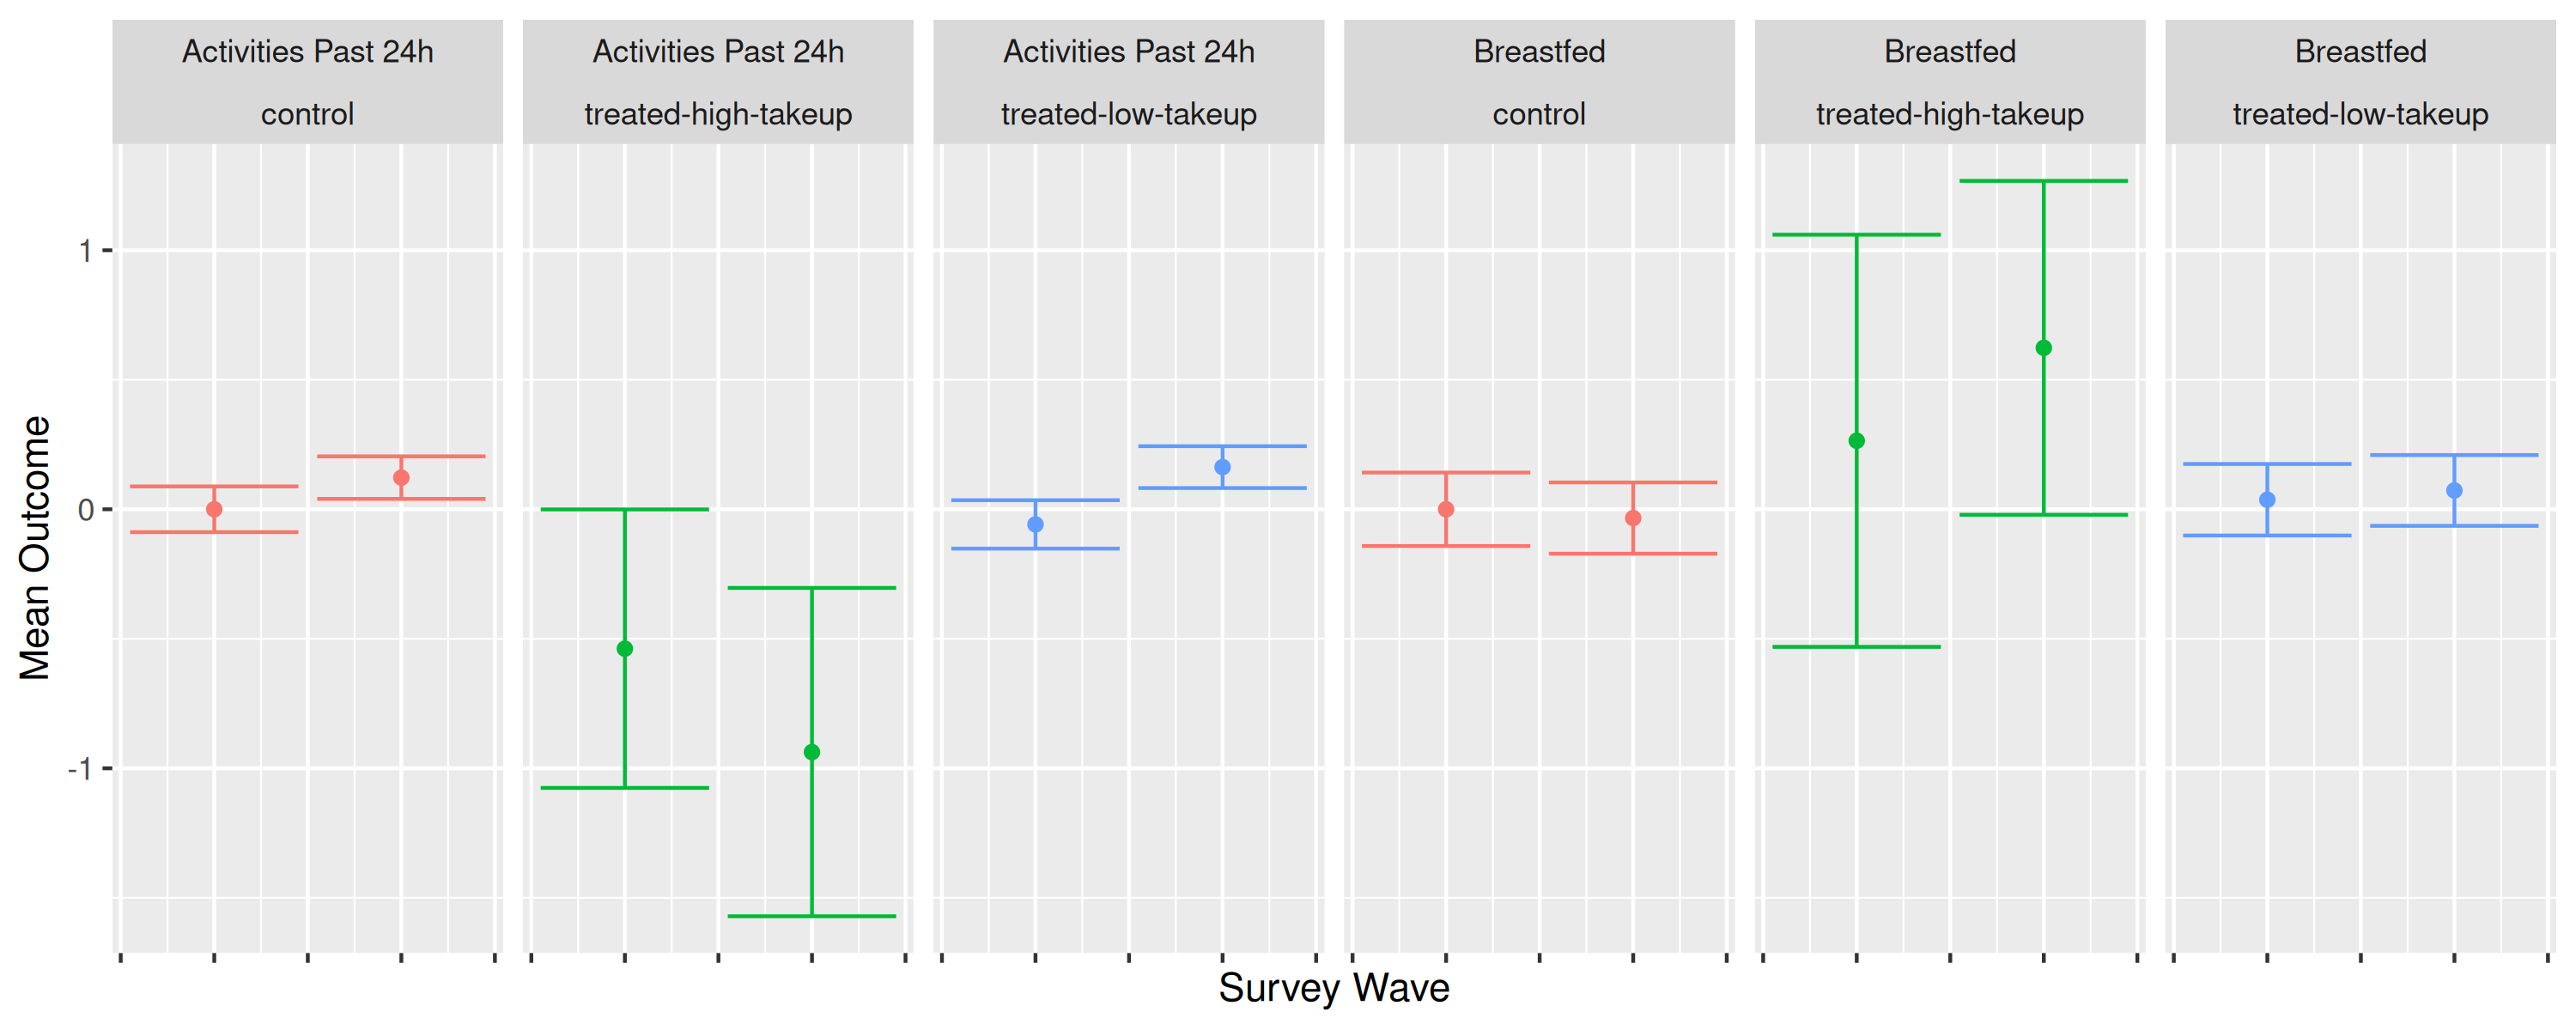
\includegraphics[width=0.9\textwidth]{plots/pre_post/Serbia: Breastfed.png}
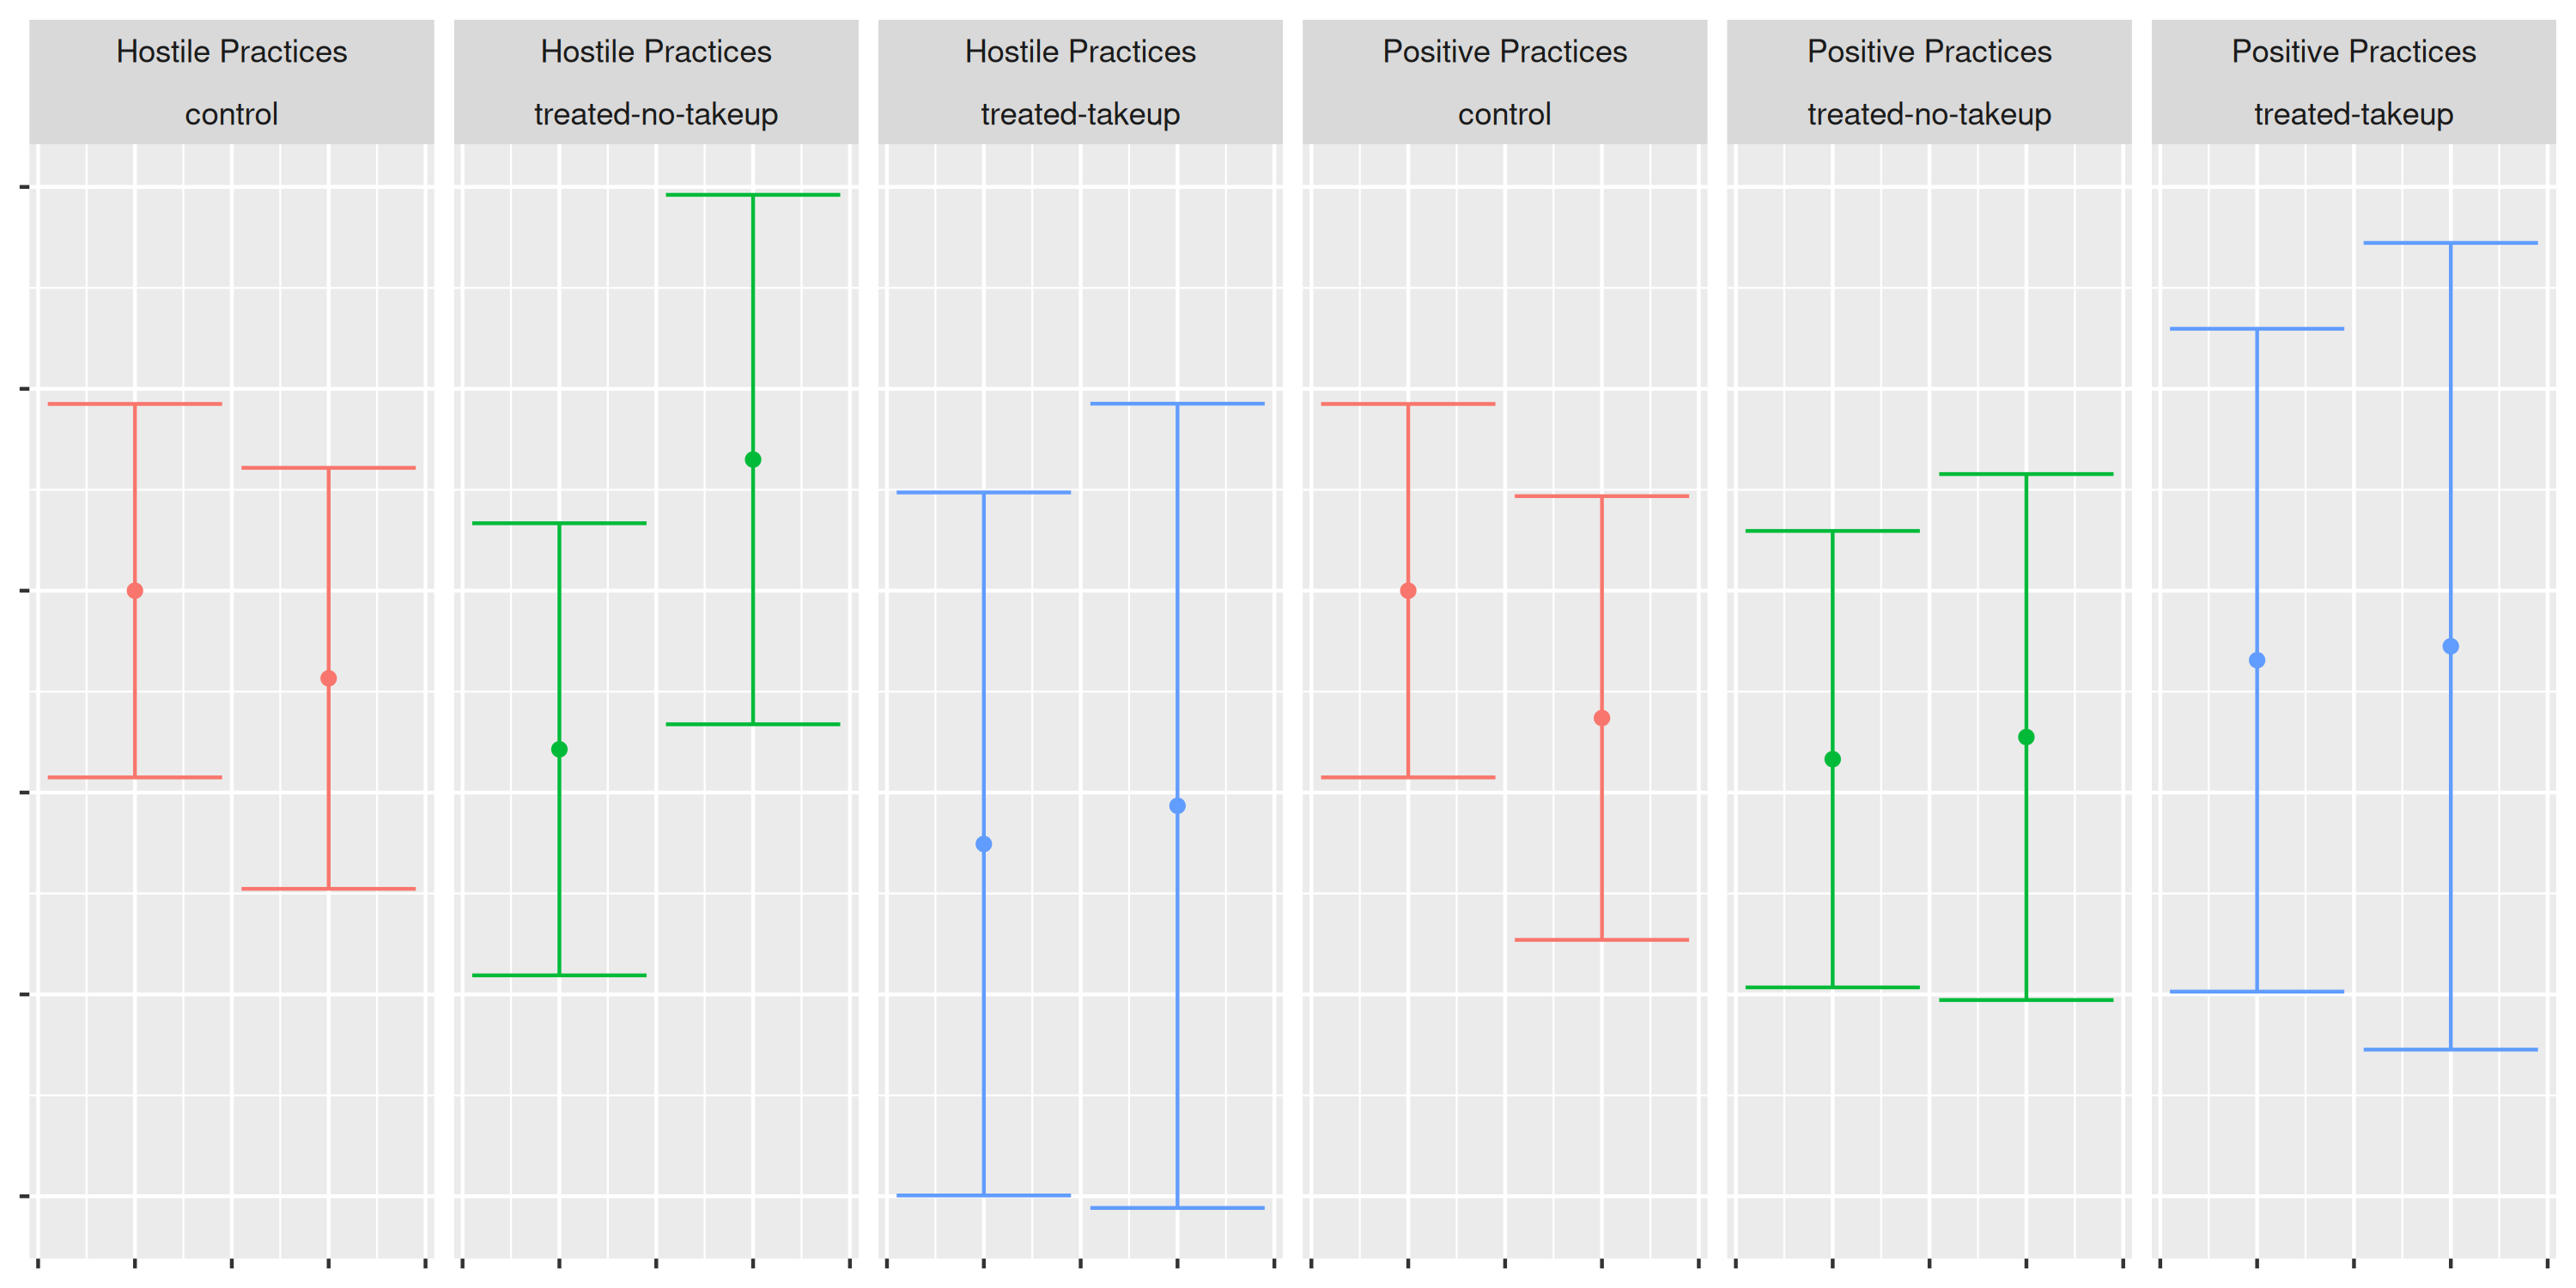
\includegraphics[width=0.9\textwidth]{plots/pre_post/Serbia: Positive Practices.png}
\end{figure}



% Table created by stargazer v.5.2.3 by Marek Hlavac, Social Policy Institute. E-mail: marek.hlavac at gmail.com
% Date and time: Sun, Jan 21, 2024 - 11:01:31 PM
\begin{table}[!htbp] \centering 
  \caption{Serbia: 2SLS - Endline - Knowledge and Awareness} 
  \label{tbl:Serbia: 2SLS - Endline - Knowledge and Awareness} 
\begin{tabular}{@{\extracolsep{5pt}}lcc} 
\\[-1.8ex]\hline 
\hline \\[-1.8ex] 
 & \multicolumn{2}{c}{\textit{Dependent variable:}} \\ 
\cline{2-3} 
\\[-1.8ex] & Vaccine Knowledge & Child Dev. Knowledge \\ 
\\[-1.8ex] & (1) & (2)\\ 
\hline \\[-1.8ex] 
 Used App & 0.35 & $-$0.03 \\ 
  & (0.20) & (0.06) \\ 
  & & \\ 
\hline \\[-1.8ex] 
Adjusted Treatment p-value & 0.4 & 0.769 \\ 
Weak instruments p-value & 8.94e-11 & 3.96e-36 \\ 
Wu-Hausman p-value & 0.198 & 0.586 \\ 
Observations & 285 & 890 \\ 
R$^{2}$ & $-$0.02 & 0.02 \\ 
\hline 
\hline \\[-1.8ex] 
\textit{Note:}  & \multicolumn{2}{r}{$^{*}$p$<$0.1; $^{**}$p$<$0.05; $^{***}$p$<$0.01} \\ 
\end{tabular} 
\end{table} 


% Table created by stargazer v.5.2.3 by Marek Hlavac, Social Policy Institute. E-mail: marek.hlavac at gmail.com
% Date and time: Sun, Jan 21, 2024 - 11:01:31 PM
\begin{table}[!htbp] \centering 
  \caption{Serbia: 2SLS - Endline - Confidence and Attitudes} 
  \label{tbl:Serbia: 2SLS - Endline - Confidence and Attitudes} 
\begin{tabular}{@{\extracolsep{5pt}}lcc} 
\\[-1.8ex]\hline 
\hline \\[-1.8ex] 
 & \multicolumn{2}{c}{\textit{Dependent variable:}} \\ 
\cline{2-3} 
\\[-1.8ex] & Parenting Confidence & Attitude to Phys. Punishment \\ 
\\[-1.8ex] & (1) & (2)\\ 
\hline \\[-1.8ex] 
 Used App & $-$0.17 & 0.15 \\ 
  & (0.15) & (0.19) \\ 
  & & \\ 
\hline \\[-1.8ex] 
Adjusted Treatment p-value & 0.4 & 0.58 \\ 
Weak instruments p-value & 1.01e-35 & 8.66e-36 \\ 
Wu-Hausman p-value & 0.192 & 0.47 \\ 
Observations & 877 & 876 \\ 
R$^{2}$ & 0.01 & 0.005 \\ 
\hline 
\hline \\[-1.8ex] 
\textit{Note:}  & \multicolumn{2}{r}{$^{*}$p$<$0.1; $^{**}$p$<$0.05; $^{***}$p$<$0.01} \\ 
\end{tabular} 
\end{table} 


% Table created by stargazer v.5.2.3 by Marek Hlavac, Social Policy Institute. E-mail: marek.hlavac at gmail.com
% Date and time: Tue, Mar 12, 2024 - 11:43:17 PM
\begin{table}[!htbp] \centering 
  \caption{Serbia: 2SLS - Endline - Practices} 
  \label{tbl:Serbia: 2SLS - Endline - Practices} 
\begin{tabular}{@{\extracolsep{5pt}}lcccc} 
\\[-1.8ex]\hline 
\hline \\[-1.8ex] 
 & \multicolumn{4}{c}{\textit{Dependent variable:}} \\ 
\cline{2-5} 
\\[-1.8ex] & Breastfed & Activities Past 24h & Positive Practices & Hostile Practices \\ 
\\[-1.8ex] & (1) & (2) & (3) & (4)\\ 
\hline \\[-1.8ex] 
 Used App & $-$0.13 & 0.38 & 0.04 & 0.20 \\ 
  & (0.17) & (0.29) & (0.22) & (0.18) \\ 
  & & & & \\ 
\hline \\[-1.8ex] 
Adjusted Treatment p-value & 0.732 & 0.711 & 0.891 & 0.711 \\ 
Weak instruments p-value & 1.95e-11 & 5.01e-34 & 2.94e-34 & 2.51e-34 \\ 
Wu-Hausman p-value & 0.609 & 0.118 & 0.941 & 0.223 \\ 
Observations & 304 & 949 & 950 & 948 \\ 
R$^{2}$ & 0.04 & $-$0.01 & 0.01 & 0.01 \\ 
\hline 
\hline \\[-1.8ex] 
\textit{Note:}  & \multicolumn{4}{r}{$^{*}$p$<$0.1; $^{**}$p$<$0.05; $^{***}$p$<$0.01} \\ 
\end{tabular} 
\end{table} 



% Table created by stargazer v.5.2.3 by Marek Hlavac, Social Policy Institute. E-mail: marek.hlavac at gmail.com
% Date and time: Sun, Feb 11, 2024 - 04:03:51 PM
\begin{table}[!htbp] \centering 
  \caption{Pooled for Follow Up: OLS - Follow Up - Knowledge and Awareness} 
  \label{tbl:Pooled for Follow Up: OLS - Follow Up - Knowledge and Awareness} 
\begin{tabular}{@{\extracolsep{5pt}}lcc} 
\\[-1.8ex]\hline 
\hline \\[-1.8ex] 
 & \multicolumn{2}{c}{\textit{Dependent variable:}} \\ 
\cline{2-3} 
\\[-1.8ex] & Vaccine Knowledge & Child Dev. Knowledge \\ 
\\[-1.8ex] & (1) & (2)\\ 
\hline \\[-1.8ex] 
 Treatment & $-$0.001 & $-$0.01 \\ 
  & (0.07) & (0.02) \\ 
  & & \\ 
\hline \\[-1.8ex] 
Adjusted Treatment p-value & 0.99 & 0.99 \\ 
Observations & 133 & 417 \\ 
R$^{2}$ & 0.03 & 0.04 \\ 
\hline 
\hline \\[-1.8ex] 
\textit{Note:}  & \multicolumn{2}{r}{$^{*}$p$<$0.1; $^{**}$p$<$0.05; $^{***}$p$<$0.01} \\ 
\end{tabular} 
\end{table} 


% Table created by stargazer v.5.2.3 by Marek Hlavac, Social Policy Institute. E-mail: marek.hlavac at gmail.com
% Date and time: Sun, Jan 21, 2024 - 11:01:41 PM
\begin{table}[!htbp] \centering 
  \caption{Pooled for Follow Up: OLS - Follow Up - Confidence and Attitudes} 
  \label{tbl:Pooled for Follow Up: OLS - Follow Up - Confidence and Attitudes} 
\begin{tabular}{@{\extracolsep{5pt}}lcc} 
\\[-1.8ex]\hline 
\hline \\[-1.8ex] 
 & \multicolumn{2}{c}{\textit{Dependent variable:}} \\ 
\cline{2-3} 
\\[-1.8ex] & Parenting Confidence & Attitude to Phys. Punishment \\ 
\\[-1.8ex] & (1) & (2)\\ 
\hline \\[-1.8ex] 
 Treatment & $-$0.05 & 0.0001 \\ 
  & (0.06) & (0.08) \\ 
  & & \\ 
\hline \\[-1.8ex] 
Adjusted Treatment p-value & 0.999 & 0.999 \\ 
Observations & 419 & 419 \\ 
R$^{2}$ & 0.04 & 0.04 \\ 
\hline 
\hline \\[-1.8ex] 
\textit{Note:}  & \multicolumn{2}{r}{$^{*}$p$<$0.1; $^{**}$p$<$0.05; $^{***}$p$<$0.01} \\ 
\end{tabular} 
\end{table} 


% Table created by stargazer v.5.2.3 by Marek Hlavac, Social Policy Institute. E-mail: marek.hlavac at gmail.com
% Date and time: Mon, Mar 18, 2024 - 11:42:23 PM
\begin{table}[!htbp] \centering 
  \caption{Pooled for Follow Up: OLS - Follow Up - Practices} 
  \label{tbl:Pooled for Follow Up: OLS - Follow Up - Practices} 
\begin{tabular}{@{\extracolsep{5pt}}lcccc} 
\\[-1.8ex]\hline 
\hline \\[-1.8ex] 
 & \multicolumn{4}{c}{\textit{Dependent variable:}} \\ 
\cline{2-5} 
\\[-1.8ex] & Breastfed & Activities Past 24h & Positive Practices & Hostile Practices \\ 
\\[-1.8ex] & (1) & (2) & (3) & (4)\\ 
\hline \\[-1.8ex] 
 Treatment & $-$0.10 & 0.09 & 0.03 & 0.01 \\ 
  & (0.06) & (0.10) & (0.07) & (0.06) \\ 
  & & & & \\ 
\hline \\[-1.8ex] 
Adjusted Treatment p-value & 0.348 & 0.821 & 0.821 & 0.821 \\ 
Observations & 188 & 558 & 558 & 557 \\ 
R$^{2}$ & 0.04 & 0.01 & 0.02 & 0.01 \\ 
\hline 
\hline \\[-1.8ex] 
\textit{Note:}  & \multicolumn{4}{r}{$^{*}$p$<$0.1; $^{**}$p$<$0.05; $^{***}$p$<$0.01} \\ 
\end{tabular} 
\end{table} 



% Table created by stargazer v.5.2.3 by Marek Hlavac, Social Policy Institute. E-mail: marek.hlavac at gmail.com
% Date and time: Tue, Mar 12, 2024 - 11:43:42 PM
\begin{table}[!htbp] \centering 
  \caption{Pooled for Follow Up: 2SLS - Follow Up - Knowledge and Awareness} 
  \label{tbl:Pooled for Follow Up: 2SLS - Follow Up - Knowledge and Awareness} 
\begin{tabular}{@{\extracolsep{5pt}}lcc} 
\\[-1.8ex]\hline 
\hline \\[-1.8ex] 
 & \multicolumn{2}{c}{\textit{Dependent variable:}} \\ 
\cline{2-3} 
\\[-1.8ex] & Vaccine Knowledge & Child Dev. Knowledge \\ 
\\[-1.8ex] & (1) & (2)\\ 
\hline \\[-1.8ex] 
 Used App & 0.36 & $-$0.01 \\ 
  & (0.20) & (0.07) \\ 
  & & \\ 
\hline \\[-1.8ex] 
Adjusted Treatment p-value & 0.388 & 0.821 \\ 
Weak instruments p-value & 5.14e-10 & 2.66e-28 \\ 
Wu-Hausman p-value & 0.346 & 0.406 \\ 
Observations & 189 & 562 \\ 
R$^{2}$ & 0.02 & 0.02 \\ 
\hline 
\hline \\[-1.8ex] 
\textit{Note:}  & \multicolumn{2}{r}{$^{*}$p$<$0.1; $^{**}$p$<$0.05; $^{***}$p$<$0.01} \\ 
\end{tabular} 
\end{table} 


% Table created by stargazer v.5.2.3 by Marek Hlavac, Social Policy Institute. E-mail: marek.hlavac at gmail.com
% Date and time: Mon, Mar 18, 2024 - 11:42:31 PM
\begin{table}[!htbp] \centering 
  \caption{Pooled for Follow Up: 2SLS - Follow Up - Confidence and Attitudes} 
  \label{tbl:Pooled for Follow Up: 2SLS - Follow Up - Confidence and Attitudes} 
\begin{tabular}{@{\extracolsep{5pt}}lcc} 
\\[-1.8ex]\hline 
\hline \\[-1.8ex] 
 & \multicolumn{2}{c}{\textit{Dependent variable:}} \\ 
\cline{2-3} 
\\[-1.8ex] & Parenting Confidence & Attitude to Phys. Punishment \\ 
\\[-1.8ex] & (1) & (2)\\ 
\hline \\[-1.8ex] 
 Used App & 0.08 & 0.14 \\ 
  & (0.18) & (0.25) \\ 
  & & \\ 
\hline \\[-1.8ex] 
Adjusted Treatment p-value & 0.821 & 0.821 \\ 
Weak instruments p-value & 6.39e-28 & 7.23e-28 \\ 
Wu-Hausman p-value & 0.699 & 0.643 \\ 
Observations & 561 & 560 \\ 
R$^{2}$ & 0.03 & 0.03 \\ 
\hline 
\hline \\[-1.8ex] 
\textit{Note:}  & \multicolumn{2}{r}{$^{*}$p$<$0.1; $^{**}$p$<$0.05; $^{***}$p$<$0.01} \\ 
\end{tabular} 
\end{table} 


% Table created by stargazer v.5.2.3 by Marek Hlavac, Social Policy Institute. E-mail: marek.hlavac at gmail.com
% Date and time: Mon, Mar 11, 2024 - 09:44:09 PM
\begin{table}[!htbp] \centering 
  \caption{Pooled for Follow Up: 2SLS - Follow Up - Practices} 
  \label{tbl:Pooled for Follow Up: 2SLS - Follow Up - Practices} 
\begin{tabular}{@{\extracolsep{5pt}}lcccc} 
\\[-1.8ex]\hline 
\hline \\[-1.8ex] 
 & \multicolumn{4}{c}{\textit{Dependent variable:}} \\ 
\cline{2-5} 
\\[-1.8ex] & Breastfed & Activities Past 24h & Positive Practices & Hostile Practices \\ 
\\[-1.8ex] & (1) & (2) & (3) & (4)\\ 
\hline \\[-1.8ex] 
 Used App & $-$0.44 & 0.22 & $-$0.004 & $-$0.12 \\ 
  & (0.31) & (0.47) & (0.30) & (0.26) \\ 
  & & & & \\ 
\hline \\[-1.8ex] 
Adjusted Treatment p-value & 0.99 & 0.99 & 0.99 & 0.99 \\ 
Weak instruments p-value & 4.16e-05 & 1.03e-16 & 1.03e-16 & 8.65e-17 \\ 
Wu-Hausman p-value & 0.472 & 0.885 & 0.663 & 0.966 \\ 
Observations & 132 & 414 & 414 & 413 \\ 
R$^{2}$ & 0.02 & 0.01 & 0.03 & 0.02 \\ 
\hline 
\hline \\[-1.8ex] 
\textit{Note:}  & \multicolumn{4}{r}{$^{*}$p$<$0.1; $^{**}$p$<$0.05; $^{***}$p$<$0.01} \\ 
\end{tabular} 
\end{table} 



% 
% Table created by stargazer v.5.2.3 by Marek Hlavac, Social Policy Institute. E-mail: marek.hlavac at gmail.com
% Date and time: Tue, Mar 12, 2024 - 11:43:09 PM
\begin{table}[!htbp] \centering 
  \caption{Bulgaria: OLS - Endline - Knowledge and Awareness} 
  \label{tbl:Bulgaria: OLS - Endline - Knowledge and Awareness} 
\begin{tabular}{@{\extracolsep{5pt}}lcc} 
\\[-1.8ex]\hline 
\hline \\[-1.8ex] 
 & \multicolumn{2}{c}{\textit{Dependent variable:}} \\ 
\cline{2-3} 
\\[-1.8ex] & Vaccine Knowledge & Child Dev. Knowledge \\ 
\\[-1.8ex] & (1) & (2)\\ 
\hline \\[-1.8ex] 
 Treatment & $-$0.04 & 0.01 \\ 
  & (0.06) & (0.02) \\ 
  & & \\ 
\hline \\[-1.8ex] 
Adjusted Treatment p-value & 0.746 & 0.797 \\ 
Observations & 256 & 678 \\ 
R$^{2}$ & 0.04 & 0.01 \\ 
\hline 
\hline \\[-1.8ex] 
\textit{Note:}  & \multicolumn{2}{r}{$^{*}$p$<$0.1; $^{**}$p$<$0.05; $^{***}$p$<$0.01} \\ 
\end{tabular} 
\end{table} 

% 
% Table created by stargazer v.5.2.3 by Marek Hlavac, Social Policy Institute. E-mail: marek.hlavac at gmail.com
% Date and time: Tue, Mar 12, 2024 - 11:43:10 PM
\begin{table}[!htbp] \centering 
  \caption{Bulgaria: OLS - Endline - Confidence and Attitudes} 
  \label{tbl:Bulgaria: OLS - Endline - Confidence and Attitudes} 
\begin{tabular}{@{\extracolsep{5pt}}lcc} 
\\[-1.8ex]\hline 
\hline \\[-1.8ex] 
 & \multicolumn{2}{c}{\textit{Dependent variable:}} \\ 
\cline{2-3} 
\\[-1.8ex] & Parenting Confidence & Attitude to Phys. Punishment \\ 
\\[-1.8ex] & (1) & (2)\\ 
\hline \\[-1.8ex] 
 Treatment & 0.07 & 0.13 \\ 
  & (0.05) & (0.07) \\ 
  & & \\ 
\hline \\[-1.8ex] 
Adjusted Treatment p-value & 0.338 & 0.336 \\ 
Observations & 665 & 657 \\ 
R$^{2}$ & 0.01 & 0.02 \\ 
\hline 
\hline \\[-1.8ex] 
\textit{Note:}  & \multicolumn{2}{r}{$^{*}$p$<$0.1; $^{**}$p$<$0.05; $^{***}$p$<$0.01} \\ 
\end{tabular} 
\end{table} 

% 
% Table created by stargazer v.5.2.3 by Marek Hlavac, Social Policy Institute. E-mail: marek.hlavac at gmail.com
% Date and time: Mon, Mar 11, 2024 - 09:43:50 PM
\begin{table}[!htbp] \centering 
  \caption{Bulgaria: OLS - Endline - Practices} 
  \label{tbl:Bulgaria: OLS - Endline - Practices} 
\begin{tabular}{@{\extracolsep{5pt}}lcccc} 
\\[-1.8ex]\hline 
\hline \\[-1.8ex] 
 & \multicolumn{4}{c}{\textit{Dependent variable:}} \\ 
\cline{2-5} 
\\[-1.8ex] & Breastfed & Activities Past 24h & Positive Practices & Hostile Practices \\ 
\\[-1.8ex] & (1) & (2) & (3) & (4)\\ 
\hline \\[-1.8ex] 
 Treatment & 0.08 & 0.11 & $-$0.01 & 0.06 \\ 
  & (0.04) & (0.10) & (0.03) & (0.05) \\ 
  & & & & \\ 
\hline \\[-1.8ex] 
Adjusted Treatment p-value & 0.336 & 0.396 & 0.822 & 0.396 \\ 
Observations & 234 & 629 & 629 & 627 \\ 
R$^{2}$ & 0.10 & 0.03 & 0.05 & 0.01 \\ 
\hline 
\hline \\[-1.8ex] 
\textit{Note:}  & \multicolumn{4}{r}{$^{*}$p$<$0.1; $^{**}$p$<$0.05; $^{***}$p$<$0.01} \\ 
\end{tabular} 
\end{table} 


% 
% Table created by stargazer v.5.2.3 by Marek Hlavac, Social Policy Institute. E-mail: marek.hlavac at gmail.com
% Date and time: Mon, Mar 11, 2024 - 09:43:54 PM
\begin{table}[!htbp] \centering 
  \caption{Bulgaria: 2SLS - Endline - Knowledge and Awareness} 
  \label{tbl:Bulgaria: 2SLS - Endline - Knowledge and Awareness} 
\begin{tabular}{@{\extracolsep{5pt}}lcc} 
\\[-1.8ex]\hline 
\hline \\[-1.8ex] 
 & \multicolumn{2}{c}{\textit{Dependent variable:}} \\ 
\cline{2-3} 
\\[-1.8ex] & Vaccine Knowledge & Child Dev. Knowledge \\ 
\\[-1.8ex] & (1) & (2)\\ 
\hline \\[-1.8ex] 
 Used App & $-$0.10 & 0.01 \\ 
  & (0.17) & (0.07) \\ 
  & & \\ 
\hline \\[-1.8ex] 
Adjusted Treatment p-value & 0.748 & 0.855 \\ 
Weak instruments p-value & 4.17e-14 & 2.91e-30 \\ 
Wu-Hausman p-value & 0.448 & 0.934 \\ 
Observations & 256 & 677 \\ 
R$^{2}$ & 0.03 & 0.01 \\ 
\hline 
\hline \\[-1.8ex] 
\textit{Note:}  & \multicolumn{2}{r}{$^{*}$p$<$0.1; $^{**}$p$<$0.05; $^{***}$p$<$0.01} \\ 
\end{tabular} 
\end{table} 

% 
% Table created by stargazer v.5.2.3 by Marek Hlavac, Social Policy Institute. E-mail: marek.hlavac at gmail.com
% Date and time: Mon, Mar 18, 2024 - 11:42:11 PM
\begin{table}[!htbp] \centering 
  \caption{Bulgaria: 2SLS - Endline - Confidence and Attitudes} 
  \label{tbl:Bulgaria: 2SLS - Endline - Confidence and Attitudes} 
\begin{tabular}{@{\extracolsep{5pt}}lcc} 
\\[-1.8ex]\hline 
\hline \\[-1.8ex] 
 & \multicolumn{2}{c}{\textit{Dependent variable:}} \\ 
\cline{2-3} 
\\[-1.8ex] & Parenting Confidence & Attitude to Phys. Punishment \\ 
\\[-1.8ex] & (1) & (2)\\ 
\hline \\[-1.8ex] 
 Used App & 0.23 & 0.39 \\ 
  & (0.15) & (0.21) \\ 
  & & \\ 
\hline \\[-1.8ex] 
Adjusted Treatment p-value & 0.342 & 0.342 \\ 
Weak instruments p-value & 1.16e-33 & 5.23e-34 \\ 
Wu-Hausman p-value & 0.299 & 0.126 \\ 
Observations & 665 & 657 \\ 
R$^{2}$ & 0.01 & 0.003 \\ 
\hline 
\hline \\[-1.8ex] 
\textit{Note:}  & \multicolumn{2}{r}{$^{*}$p$<$0.1; $^{**}$p$<$0.05; $^{***}$p$<$0.01} \\ 
\end{tabular} 
\end{table} 

% 
% Table created by stargazer v.5.2.3 by Marek Hlavac, Social Policy Institute. E-mail: marek.hlavac at gmail.com
% Date and time: Mon, Mar 18, 2024 - 11:42:12 PM
\begin{table}[!htbp] \centering 
  \caption{Bulgaria: 2SLS - Endline - Practices} 
  \label{tbl:Bulgaria: 2SLS - Endline - Practices} 
\begin{tabular}{@{\extracolsep{5pt}}lcccc} 
\\[-1.8ex]\hline 
\hline \\[-1.8ex] 
 & \multicolumn{4}{c}{\textit{Dependent variable:}} \\ 
\cline{2-5} 
\\[-1.8ex] & Breastfed & Activities Past 24h & Positive Practices & Hostile Practices \\ 
\\[-1.8ex] & (1) & (2) & (3) & (4)\\ 
\hline \\[-1.8ex] 
 Used App & 0.20 & 0.36 & $-$0.04 & 0.18 \\ 
  & (0.12) & (0.31) & (0.10) & (0.14) \\ 
  & & & & \\ 
\hline \\[-1.8ex] 
Adjusted Treatment p-value & 0.342 & 0.4 & 0.797 & 0.4 \\ 
Weak instruments p-value & 6.97e-15 & 3.6e-32 & 3.6e-32 & 3.19e-32 \\ 
Wu-Hausman p-value & 0.0807 & 0.24 & 0.812 & 0.129 \\ 
Observations & 234 & 629 & 629 & 627 \\ 
R$^{2}$ & 0.05 & 0.02 & 0.06 & $-$0.003 \\ 
\hline 
\hline \\[-1.8ex] 
\textit{Note:}  & \multicolumn{4}{r}{$^{*}$p$<$0.1; $^{**}$p$<$0.05; $^{***}$p$<$0.01} \\ 
\end{tabular} 
\end{table} 



% 
% Table created by stargazer v.5.2.3 by Marek Hlavac, Social Policy Institute. E-mail: marek.hlavac at gmail.com
% Date and time: Sun, Nov 26, 2023 - 09:26:34 PM
\begin{table}[!htbp] \centering 
  \caption{Serbia: OLS - Follow Up - Knowledge and Awareness} 
  \label{tbl:Serbia: OLS - Follow Up - Knowledge and Awareness} 
\begin{tabular}{@{\extracolsep{5pt}}lcc} 
\\[-1.8ex]\hline 
\hline \\[-1.8ex] 
 & \multicolumn{2}{c}{\textit{Dependent variable:}} \\ 
\cline{2-3} 
\\[-1.8ex] & Vaccine Knowledge & Child Dev. Knowledge \\ 
\\[-1.8ex] & (1) & (2)\\ 
\hline \\[-1.8ex] 
 Treatment & $-$0.03 & $-$0.01 \\ 
  & (0.07) & (0.02) \\ 
  & & \\ 
\hline \\[-1.8ex] 
Adjusted Treatment p-value & 0.935 & 0.935 \\ 
Observations & 121 & 385 \\ 
R$^{2}$ & 0.04 & 0.04 \\ 
\hline 
\hline \\[-1.8ex] 
\textit{Note:}  & \multicolumn{2}{r}{$^{*}$p$<$0.1; $^{**}$p$<$0.05; $^{***}$p$<$0.01} \\ 
\end{tabular} 
\end{table} 

% 
% Table created by stargazer v.5.2.3 by Marek Hlavac, Social Policy Institute. E-mail: marek.hlavac at gmail.com
% Date and time: Wed, Jan 24, 2024 - 09:15:10 PM
\begin{table}[!htbp] \centering 
  \caption{Serbia: OLS - Follow Up - Confidence and Attitudes} 
  \label{tbl:Serbia: OLS - Follow Up - Confidence and Attitudes} 
\begin{tabular}{@{\extracolsep{5pt}}lcc} 
\\[-1.8ex]\hline 
\hline \\[-1.8ex] 
 & \multicolumn{2}{c}{\textit{Dependent variable:}} \\ 
\cline{2-3} 
\\[-1.8ex] & Parenting Confidence & Attitude to Phys. Punishment \\ 
\\[-1.8ex] & (1) & (2)\\ 
\hline \\[-1.8ex] 
 Treatment & $-$0.07 & 0.07 \\ 
  & (0.06) & (0.08) \\ 
  & & \\ 
\hline \\[-1.8ex] 
Adjusted Treatment p-value & 0.899 & 0.899 \\ 
Observations & 383 & 383 \\ 
R$^{2}$ & 0.05 & 0.03 \\ 
\hline 
\hline \\[-1.8ex] 
\textit{Note:}  & \multicolumn{2}{r}{$^{*}$p$<$0.1; $^{**}$p$<$0.05; $^{***}$p$<$0.01} \\ 
\end{tabular} 
\end{table} 

% 
% Table created by stargazer v.5.2.3 by Marek Hlavac, Social Policy Institute. E-mail: marek.hlavac at gmail.com
% Date and time: Sun, Nov 26, 2023 - 09:26:34 PM
\begin{table}[!htbp] \centering 
  \caption{Serbia: OLS - Follow Up - Practices} 
  \label{tbl:Serbia: OLS - Follow Up - Practices} 
\begin{tabular}{@{\extracolsep{5pt}}lcccc} 
\\[-1.8ex]\hline 
\hline \\[-1.8ex] 
 & \multicolumn{4}{c}{\textit{Dependent variable:}} \\ 
\cline{2-5} 
\\[-1.8ex] & Breastfed & Activities Past 24h & Positive Practices & Hostile Practices \\ 
\\[-1.8ex] & (1) & (2) & (3) & (4)\\ 
\hline \\[-1.8ex] 
 Treatment & $-$0.13 & 0.03 & 0.01 & 0.01 \\ 
  & (0.07) & (0.13) & (0.08) & (0.07) \\ 
  & & & & \\ 
\hline \\[-1.8ex] 
Adjusted Treatment p-value & 0.493 & 0.935 & 0.935 & 0.935 \\ 
Observations & 121 & 382 & 382 & 381 \\ 
R$^{2}$ & 0.05 & 0.01 & 0.04 & 0.03 \\ 
\hline 
\hline \\[-1.8ex] 
\textit{Note:}  & \multicolumn{4}{r}{$^{*}$p$<$0.1; $^{**}$p$<$0.05; $^{***}$p$<$0.01} \\ 
\end{tabular} 
\end{table} 


% 
% Table created by stargazer v.5.2.3 by Marek Hlavac, Social Policy Institute. E-mail: marek.hlavac at gmail.com
% Date and time: Sun, Jan 21, 2024 - 11:01:42 PM
\begin{table}[!htbp] \centering 
  \caption{Serbia: 2SLS - Follow Up - Knowledge and Awareness} 
  \label{tbl:Serbia: 2SLS - Follow Up - Knowledge and Awareness} 
\begin{tabular}{@{\extracolsep{5pt}}lcc} 
\\[-1.8ex]\hline 
\hline \\[-1.8ex] 
 & \multicolumn{2}{c}{\textit{Dependent variable:}} \\ 
\cline{2-3} 
\\[-1.8ex] & Vaccine Knowledge & Child Dev. Knowledge \\ 
\\[-1.8ex] & (1) & (2)\\ 
\hline \\[-1.8ex] 
 Used App & $-$0.17 & $-$0.05 \\ 
  & (0.36) & (0.09) \\ 
  & & \\ 
\hline \\[-1.8ex] 
Adjusted Treatment p-value & 0.899 & 0.899 \\ 
Weak instruments p-value & 0.000204 & 5.33e-15 \\ 
Wu-Hausman p-value & 0.302 & 0.459 \\ 
Observations & 121 & 384 \\ 
R$^{2}$ & $-$0.02 & 0.03 \\ 
\hline 
\hline \\[-1.8ex] 
\textit{Note:}  & \multicolumn{2}{r}{$^{*}$p$<$0.1; $^{**}$p$<$0.05; $^{***}$p$<$0.01} \\ 
\end{tabular} 
\end{table} 

% 
% Table created by stargazer v.5.2.3 by Marek Hlavac, Social Policy Institute. E-mail: marek.hlavac at gmail.com
% Date and time: Wed, Jan 24, 2024 - 09:15:14 PM
\begin{table}[!htbp] \centering 
  \caption{Serbia: 2SLS - Follow Up - Confidence and Attitudes} 
  \label{tbl:Serbia: 2SLS - Follow Up - Confidence and Attitudes} 
\begin{tabular}{@{\extracolsep{5pt}}lcc} 
\\[-1.8ex]\hline 
\hline \\[-1.8ex] 
 & \multicolumn{2}{c}{\textit{Dependent variable:}} \\ 
\cline{2-3} 
\\[-1.8ex] & Parenting Confidence & Attitude to Phys. Punishment \\ 
\\[-1.8ex] & (1) & (2)\\ 
\hline \\[-1.8ex] 
 Used App & $-$0.26 & 0.26 \\ 
  & (0.26) & (0.34) \\ 
  & & \\ 
\hline \\[-1.8ex] 
Adjusted Treatment p-value & 0.899 & 0.899 \\ 
Weak instruments p-value & 1.3e-14 & 1.3e-14 \\ 
Wu-Hausman p-value & 0.344 & 0.551 \\ 
Observations & 383 & 383 \\ 
R$^{2}$ & 0.03 & 0.03 \\ 
\hline 
\hline \\[-1.8ex] 
\textit{Note:}  & \multicolumn{2}{r}{$^{*}$p$<$0.1; $^{**}$p$<$0.05; $^{***}$p$<$0.01} \\ 
\end{tabular} 
\end{table} 

% 
% Table created by stargazer v.5.2.3 by Marek Hlavac, Social Policy Institute. E-mail: marek.hlavac at gmail.com
% Date and time: Sun, Nov 26, 2023 - 09:26:37 PM
\begin{table}[!htbp] \centering 
  \caption{Serbia: 2SLS - Follow Up - Practices} 
  \label{tbl:Serbia: 2SLS - Follow Up - Practices} 
\begin{tabular}{@{\extracolsep{5pt}}lcccc} 
\\[-1.8ex]\hline 
\hline \\[-1.8ex] 
 & \multicolumn{4}{c}{\textit{Dependent variable:}} \\ 
\cline{2-5} 
\\[-1.8ex] & Breastfed & Activities Past 24h & Positive Practices & Hostile Practices \\ 
\\[-1.8ex] & (1) & (2) & (3) & (4)\\ 
\hline \\[-1.8ex] 
 Used App & $-$0.67 & 0.11 & 0.06 & 0.02 \\ 
  & (0.37) & (0.51) & (0.34) & (0.29) \\ 
  & & & & \\ 
\hline \\[-1.8ex] 
Adjusted Treatment p-value & 0.588 & 0.935 & 0.935 & 0.935 \\ 
Weak instruments p-value & 0.000204 & 3.43e-14 & 3.43e-14 & 2.96e-14 \\ 
Wu-Hausman p-value & 0.22 & 0.949 & 0.795 & 0.594 \\ 
Observations & 121 & 382 & 382 & 381 \\ 
R$^{2}$ & $-$0.04 & 0.01 & 0.04 & 0.03 \\ 
\hline 
\hline \\[-1.8ex] 
\textit{Note:}  & \multicolumn{4}{r}{$^{*}$p$<$0.1; $^{**}$p$<$0.05; $^{***}$p$<$0.01} \\ 
\end{tabular} 
\end{table} 


% 
% Table created by stargazer v.5.2.3 by Marek Hlavac, Social Policy Institute. E-mail: marek.hlavac at gmail.com
% Date and time: Sun, Jan 21, 2024 - 11:01:39 PM
\begin{table}[!htbp] \centering 
  \caption{Bulgaria: OLS - Follow Up - Knowledge and Awareness} 
  \label{tbl:Bulgaria: OLS - Follow Up - Knowledge and Awareness} 
\begin{tabular}{@{\extracolsep{5pt}}lcc} 
\\[-1.8ex]\hline 
\hline \\[-1.8ex] 
 & \multicolumn{2}{c}{\textit{Dependent variable:}} \\ 
\cline{2-3} 
\\[-1.8ex] & Vaccine Knowledge & Child Dev. Knowledge \\ 
\\[-1.8ex] & (1) & (2)\\ 
\hline \\[-1.8ex] 
 Treatment & $-$0.06 & 0.03 \\ 
  & (0.10) & (0.03) \\ 
  & & \\ 
\hline \\[-1.8ex] 
Adjusted Treatment p-value & 0.708 & 0.575 \\ 
Observations & 123 & 328 \\ 
R$^{2}$ & 0.08 & 0.04 \\ 
\hline 
\hline \\[-1.8ex] 
\textit{Note:}  & \multicolumn{2}{r}{$^{*}$p$<$0.1; $^{**}$p$<$0.05; $^{***}$p$<$0.01} \\ 
\end{tabular} 
\end{table} 

% 
% Table created by stargazer v.5.2.3 by Marek Hlavac, Social Policy Institute. E-mail: marek.hlavac at gmail.com
% Date and time: Sun, Nov 26, 2023 - 09:26:34 PM
\begin{table}[!htbp] \centering 
  \caption{Bulgaria: OLS - Follow Up - Confidence and Attitudes} 
  \label{tbl:Bulgaria: OLS - Follow Up - Confidence and Attitudes} 
\begin{tabular}{@{\extracolsep{5pt}}lcc} 
\\[-1.8ex]\hline 
\hline \\[-1.8ex] 
 & \multicolumn{2}{c}{\textit{Dependent variable:}} \\ 
\cline{2-3} 
\\[-1.8ex] & Parenting Confidence & Attitude to Phys. Punishment \\ 
\\[-1.8ex] & (1) & (2)\\ 
\hline \\[-1.8ex] 
 Treatment & 0.11 & 0.17 \\ 
  & (0.07) & (0.11) \\ 
  & & \\ 
\hline \\[-1.8ex] 
Adjusted Treatment p-value & 0.407 & 0.407 \\ 
Observations & 323 & 323 \\ 
R$^{2}$ & 0.03 & 0.04 \\ 
\hline 
\hline \\[-1.8ex] 
\textit{Note:}  & \multicolumn{2}{r}{$^{*}$p$<$0.1; $^{**}$p$<$0.05; $^{***}$p$<$0.01} \\ 
\end{tabular} 
\end{table} 

% 
% Table created by stargazer v.5.2.3 by Marek Hlavac, Social Policy Institute. E-mail: marek.hlavac at gmail.com
% Date and time: Sun, Nov 26, 2023 - 09:26:35 PM
\begin{table}[!htbp] \centering 
  \caption{Bulgaria: OLS - Follow Up - Practices} 
  \label{tbl:Bulgaria: OLS - Follow Up - Practices} 
\begin{tabular}{@{\extracolsep{5pt}}lcccc} 
\\[-1.8ex]\hline 
\hline \\[-1.8ex] 
 & \multicolumn{4}{c}{\textit{Dependent variable:}} \\ 
\cline{2-5} 
\\[-1.8ex] & Breastfed & Activities Past 24h & Positive Practices & Hostile Practices \\ 
\\[-1.8ex] & (1) & (2) & (3) & (4)\\ 
\hline \\[-1.8ex] 
 Treatment & 0.04 & 0.26 & 0.03 & 0.02 \\ 
  & (0.06) & (0.16) & (0.05) & (0.07) \\ 
  & & & & \\ 
\hline \\[-1.8ex] 
Adjusted Treatment p-value & 0.708 & 0.407 & 0.708 & 0.722 \\ 
Observations & 117 & 320 & 320 & 320 \\ 
R$^{2}$ & 0.16 & 0.05 & 0.06 & 0.03 \\ 
\hline 
\hline \\[-1.8ex] 
\textit{Note:}  & \multicolumn{4}{r}{$^{*}$p$<$0.1; $^{**}$p$<$0.05; $^{***}$p$<$0.01} \\ 
\end{tabular} 
\end{table} 


% 
% Table created by stargazer v.5.2.3 by Marek Hlavac, Social Policy Institute. E-mail: marek.hlavac at gmail.com
% Date and time: Sun, Jan 21, 2024 - 11:01:44 PM
\begin{table}[!htbp] \centering 
  \caption{Bulgaria: 2SLS - Follow Up - Knowledge and Awareness} 
  \label{tbl:Bulgaria: 2SLS - Follow Up - Knowledge and Awareness} 
\begin{tabular}{@{\extracolsep{5pt}}lcc} 
\\[-1.8ex]\hline 
\hline \\[-1.8ex] 
 & \multicolumn{2}{c}{\textit{Dependent variable:}} \\ 
\cline{2-3} 
\\[-1.8ex] & Vaccine Knowledge & Child Dev. Knowledge \\ 
\\[-1.8ex] & (1) & (2)\\ 
\hline \\[-1.8ex] 
 Used App & $-$0.19 & 0.12 \\ 
  & (0.34) & (0.12) \\ 
  & & \\ 
\hline \\[-1.8ex] 
Adjusted Treatment p-value & 0.709 & 0.591 \\ 
Weak instruments p-value & 4.22e-06 & 6.96e-14 \\ 
Wu-Hausman p-value & 0.631 & 0.172 \\ 
Observations & 123 & 328 \\ 
R$^{2}$ & 0.07 & 0.01 \\ 
\hline 
\hline \\[-1.8ex] 
\textit{Note:}  & \multicolumn{2}{r}{$^{*}$p$<$0.1; $^{**}$p$<$0.05; $^{***}$p$<$0.01} \\ 
\end{tabular} 
\end{table} 

% 
% Table created by stargazer v.5.2.3 by Marek Hlavac, Social Policy Institute. E-mail: marek.hlavac at gmail.com
% Date and time: Wed, Jan 24, 2024 - 09:15:16 PM
\begin{table}[!htbp] \centering 
  \caption{Bulgaria: 2SLS - Follow Up - Confidence and Attitudes} 
  \label{tbl:Bulgaria: 2SLS - Follow Up - Confidence and Attitudes} 
\begin{tabular}{@{\extracolsep{5pt}}lcc} 
\\[-1.8ex]\hline 
\hline \\[-1.8ex] 
 & \multicolumn{2}{c}{\textit{Dependent variable:}} \\ 
\cline{2-3} 
\\[-1.8ex] & Parenting Confidence & Attitude to Phys. Punishment \\ 
\\[-1.8ex] & (1) & (2)\\ 
\hline \\[-1.8ex] 
 Used App & 0.39 & 0.60 \\ 
  & (0.27) & (0.42) \\ 
  & & \\ 
\hline \\[-1.8ex] 
Adjusted Treatment p-value & 0.403 & 0.403 \\ 
Weak instruments p-value & 6.66e-14 & 6.66e-14 \\ 
Wu-Hausman p-value & 0.136 & 0.103 \\ 
Observations & 324 & 324 \\ 
R$^{2}$ & $-$0.01 & $-$0.01 \\ 
\hline 
\hline \\[-1.8ex] 
\textit{Note:}  & \multicolumn{2}{r}{$^{*}$p$<$0.1; $^{**}$p$<$0.05; $^{***}$p$<$0.01} \\ 
\end{tabular} 
\end{table} 

% 
% Table created by stargazer v.5.2.3 by Marek Hlavac, Social Policy Institute. E-mail: marek.hlavac at gmail.com
% Date and time: Sun, Nov 26, 2023 - 09:26:39 PM
\begin{table}[!htbp] \centering 
  \caption{Bulgaria: 2SLS - Follow Up - Practices} 
  \label{tbl:Bulgaria: 2SLS - Follow Up - Practices} 
\begin{tabular}{@{\extracolsep{5pt}}lcccc} 
\\[-1.8ex]\hline 
\hline \\[-1.8ex] 
 & \multicolumn{4}{c}{\textit{Dependent variable:}} \\ 
\cline{2-5} 
\\[-1.8ex] & Breastfed & Activities Past 24h & Positive Practices & Hostile Practices \\ 
\\[-1.8ex] & (1) & (2) & (3) & (4)\\ 
\hline \\[-1.8ex] 
 Used App & 0.12 & 0.92 & 0.09 & 0.09 \\ 
  & (0.19) & (0.57) & (0.18) & (0.25) \\ 
  & & & & \\ 
\hline \\[-1.8ex] 
Adjusted Treatment p-value & 0.709 & 0.429 & 0.709 & 0.723 \\ 
Weak instruments p-value & 5.44e-06 & 3.03e-14 & 3.03e-14 & 3.03e-14 \\ 
Wu-Hausman p-value & 0.956 & 0.123 & 0.578 & 0.556 \\ 
Observations & 117 & 320 & 320 & 320 \\ 
R$^{2}$ & 0.17 & 0.003 & 0.05 & 0.03 \\ 
\hline 
\hline \\[-1.8ex] 
\textit{Note:}  & \multicolumn{4}{r}{$^{*}$p$<$0.1; $^{**}$p$<$0.05; $^{***}$p$<$0.01} \\ 
\end{tabular} 
\end{table} 



\section{Survey Instrument}


% Table created by stargazer v.5.2.3 by Marek Hlavac, Social Policy Institute. E-mail: marek.hlavac at gmail.com
% Date and time: Mon, Mar 18, 2024 - 11:41:32 PM
\begin{table}[!htbp] \centering 
  \caption{Construct Variable Mapping} 
  \label{tbl:Construct Variable Mapping} 
\begin{tabular}{@{\extracolsep{5pt}} ccc} 
\\[-1.8ex]\hline 
\hline \\[-1.8ex] 
Domain & construct\_variable & variable \\ 
\hline \\[-1.8ex] 
Knowledge and awareness & health\_knw & know\_which\_vaccine \\ 
Knowledge and awareness & dev\_knw\_recog & know\_social\_emotional\_dev \\ 
Knowledge and awareness & dev\_knw\_recog & know\_cog\_dev \\ 
Knowledge and awareness & dev\_knw\_recog & know\_phys\_dev \\ 
Knowledge and awareness & dev\_knw\_recog & know\_lang\_dev \\ 
Confidence and attitudes & confidence & confidence\_deal\_emotions \\ 
Confidence and attitudes & confidence & confidence\_respond\_misbehave \\ 
Confidence and attitudes & attitude & physical\_punishment \\ 
Confidence and attitudes & caregiver\_well\_being & parenting\_stress\_2 \\ 
Practices & was\_breastfed & breastfed \\ 
Practices & practices\_24 & past\_24h\_read \\ 
Practices & practices\_24 & past\_24h\_stories \\ 
Practices & practices\_24 & past\_24h\_sing \\ 
Practices & practices\_24 & past\_24h\_outside \\ 
Practices & practices\_24 & past\_24h\_play \\ 
Practices & practices\_24 & past\_24h\_draw \\ 
Practices & practices\_agree & laugh\_together \\ 
Practices & practices\_agree & joke\_with\_child \\ 
Practices & practices\_agree & smile\_around\_child \\ 
Practices & practices\_agree & play\_on\_floor \\ 
Practices & practices\_hostility & snap\_at\_child \\ 
Practices & practices\_hostility & lose\_patience\_punish \\ 
Practices & practices\_hostility & threaten \\ 
Practices & practices\_hostility & make\_fun\_of \\ 
\hline \\[-1.8ex] 
\end{tabular} 
\end{table} 


\end{document}